% \documentclass[11pt]{article} 
\documentclass[runningheads,smallextended]{svjour2}  % ARMA


% Be sure to use PDF Latex
\pdfoutput=1
\smartqed  % flush right qed marks, e.g. at end of proof

\journalname{Archive for Rational Mechanics and Analysis}

\renewcommand{\makeheadbox}{} % To remove title of journal

\usepackage{mystyle}
\usepackage{url}
\usepackage{LatexDefinitions}
\usepackage{LatexDefinitions_Thm}

\newcommand{\mnorm}{\mc{N}}
\newcommand{\srho}{\hat{\rho}}
\newcommand{\trucos}{{\ol{\cos}}}
\newcommand{\dens}[2]{\textstyle{\frac{#1}{#2}}}
\numberwithin{equation}{section}


\begin{document}
\title{Unbalanced Optimal Transport}
\subtitle{Geometry and Kantorovich Formulation}

\author{L\'ena\"ic~Chizat         \and
		Gabriel~Peyr\'e			\and
        Bernhard~Schmitzer 		\and
       Fran\c{c}ois-Xavier~Vialard
}
\date{}
%\author{
%\begin{tabular}{c}
%	L\'ena\"ic Chizat \qquad Gabriel Peyr\'e\\
%	Bernhard Schmitzer  \qquad Fran\c{c}ois-Xavier Vialard\\[2mm]
%	Ceremade, Universit\'e Paris-Dauphine \\
%	\texttt{\small\{chizat,peyre,schmitzer,vialard\}@ceremade.dauphine.fr}
%\end{tabular} }

\institute{Ceremade, Universit\'e Paris-Dauphine\\
              \email{\{chizat,peyre,schmitzer,vialard\}@ceremade.dauphine.fr}      
}


\maketitle

%\setcounter{tocdepth}{1}
%\tableofcontents

% !TEX root = ../InterpolatingOTFR.tex

\begin{abstract}
This paper defines a new transport metric over the space of non-negative measures. This metric interpolates between the quadratic Wasserstein and the Fisher-Rao metrics and generalizes optimal transport to measures with different masses.
%
It is defined as a generalization of the dynamical formulation of optimal transport of Benamou and Brenier, by introducing a source term in the continuity equation. The influence of this source term is measured using the Fisher-Rao metric, and is averaged with the transportation term. This gives rise to a convex variational problem defining the new metric. 
% 
Our first contribution is a proof of the existence of geodesics (i.e. solutions to this variational problem).
We then show that (generalized) optimal transport and Hellinger metrics are obtained as limiting cases of our metric.
Our last theoretical contribution is a proof that geodesics between mixtures of sufficiently close Dirac measures are made of translating mixtures of Dirac masses. 
Lastly, we propose a numerical scheme making use of first order proximal splitting methods and we show an application of this new distance to image interpolation.
\end{abstract}
% !TEX root = ../InterpolatingOTFR.tex


%\todo{Gabriel: Dans l'article, les notations $(x,t)$ et $(t,x)$ alternent. Lenaic, peux tu faire un choix et tout corriger ? DONE}

\section{Introduction}

Optimal transport is an optimization problem which gives rise to a popular class of metrics between probability distributions. We refer to the monograph of Villani~\cite{cedric2003topics} for a detailed overview of optimal transport. We now describe in an informal way various formulations of transportation-like distances, and expose also our new metric. A mathematically rigorous treatment can be found in Section~\ref{sec:theory}. 


%%%%
\subsection{Static and dynamic optimal transport}

In its original formulation by Monge, optimal transport takes into account a ground cost that measures the amount of work needed to transfer a measure towards another one.  This formulation was later relaxed by Kantorovich~\cite{Kantorovich42} as a convex linear program, often referred to as a ``static formulation''. 
%
Given a \emph{ground cost} $c : \Om^2 \mapsto \R$, $\Om \subset \R^d$ and two probability measures $\rho_0$ and $\rho_1$ on $\Om$, the central problem is that of minimizing
\begin{equation}
\int_{\Om \times \Om} c(x,y) \,\d\gamma (x,y)
\label{optimal transport problem}
\end{equation}
over the set $\Gamma_{(\rho_0,\rho_1)}$ of coupling measures, that contains non-negative measures $\gamma$ on $\Om^2$ admitting $\rho_0$ and $\rho_1$ as first and second marginals. More explicitly, for every measurable set $A \subset \Om$, $\gamma(A,\Om)=\rho_0(A)$ and $\gamma(\Om,A)=\rho_1(A)$. When the \emph{ground cost} is the distance $|x-y|^p$, the minimum induces a metric on the space of probability measures which is often referred to as the p-Wasserstein distance, denoted by $W_p$. 


In a seminal paper, Benamou and Brenier~\cite{benamou2000computational} showed that this static formulation is equivalent to a ``dynamical'' formulation, where one seeks for a ``geodesic path'' $\rho(t,x)$ between the two densities which has a convex formulation. More precisely, they showed that the squared 2-Wasserstein is obtained by minimizing the kinetic energy
\[
\int_0^1 \int_{\Omega} |v(t,x)|^2 \rho(t,x) \d x \d t
\]
where $\rho$ interpolates between $\rho_0$ and $\rho_1$ and $v$ is a velocity field which advects the mass distribution $\rho$. They introduced the key change of variables via the momentum from classical mechanics, $(\rho,v) \mapsto (\rho,\M)\defeq (\rho,\rho v)$, this amounts to minimizing the convex functional
\begin{equation}\label{eq-dynamic}
 	\int_0^1 \int_{\Omega} \frac{|\omega(t,x)|^2}{\rho(t,x)} \,\d x \d t
\end{equation}
over the couples $(\rho,\omega)$ satisfying the continuity equation 
\begin{equation}\label{eq-continuity}
	\partial_t \rho + \nabla \cdot \omega =0, \quad \rho(0,\cdot) = \rho_0, \quad \rho(1,\cdot) = \rho_1\,.
\end{equation}
In particular, their paper emphasized the Riemannian interpretation of this metric and paved the way for efficient numerical solvers.

The geometric nature of optimal transport makes this tool interesting to perform shape interpolation, especially in medical image analysis~\cite{haker2004optimal}. Even though the resulting interpolation is somewhat simplistic compared to methods based on diffeomorphic flows such as LDDMM~\cite{beg2005computing}, the fact that the problem is convex is interesting for numerical purposes and large scale applications. 
%
A notable restriction of optimal transport is however that it is only defined between measures having the same mass. This might be an issue for applications in medical imaging, where measures need not be normalized, and biophysical phenomena at stake typically involve some sort of mass creation or destruction.
% 
To date, several generalizations of optimal transport have been proposed, with various goals in mind (see Section~\ref{previous works}). However, there is currently no formulation for which geodesics can be interpreted as a joint  displacement and modification of mass. In this article, we propose to tackle this issue by interpolating between the Wasserstein and the Fisher-Rao metric, which can be achieved using a convex dynamical formulation.


In the remainder of this section, we introduce our model and describe related work which generalizes optimal transport to unbalanced measures (nonnegative measures whose total mass may differ). In addition, we introduce in an informal manner a family of distances which shows the similarity between \emph{a priori} unrelated models of transport between unbalanced measures. 
%
In Section~\ref{sec:theory}, we prove the existence of geodesics and exhibit optimality conditions. 
%
Section~\ref{sec-interpolation} is devoted to the study of the effect of varying the interpolation factor and to the limit models. 
%
We detail in Section~\ref{sec-explicit-geod} explicit geodesics between atomic measures satisfying suitable properties. 
%
Finally, we describe a numerical scheme in Section~\ref{sec-numerics} and use the distance for image interpolation experiments.





%%%%%%%%%%%%%%
%%%%%%%%%%%%%%
%%%%%%%%%%%%%%
\subsection{Presentation of the model and contributions}

The dynamical formulation~\eqref{eq-dynamic} suggests a natural way to relax the equality of mass constraint by introducing a source term $\zeta$ in the continuity equation~\eqref{eq-continuity} as follows
\[
	\D_t \rho + \nabla \cdot \M = \zeta, \quad 
	\rho(0,\cdot) = \rho_0, \quad \rho(1,\cdot) = \rho_1, 
\]
and adding a term penalizing $\zeta$ in the Benamou-Brenier functional, in the spirit of metamorphoses introduced in imaging in \cite{Metamorphosis2005}. 
As for the penalization on $\Z$, we think it is natural to look for a Lagrangian which behaves like a Riemannian metric. Riemannian metrics are natural for interpolation purposes and for applications to imaging. Moreover, the standard notion of curvature is available in a Riemannian setting and provides important information on the underlying geometry, even in the case of infinite dimensional spaces.
%We think it is natural to require the following two properties for the penalization on $\Z$:
%\begin{enumerate}
%	\item \textit{Reparametrization invariance.} As the geometrical aspect of the problem is taken care of by the optimal transport part, it is important for the penalty defined on $\zeta$ not to be sensitive to deformations of the objects.
%	\item \textit{Relation with  a Riemannian metric.} Riemannian metrics are natural for interpolation purposes and for applications to imaging. Moreover, the standard notion of curvature is available in a Riemannian setting and give important information on the underlying geometry, even in the case of infinite dimensional spaces.
%	% as they guarantee local unicity of the interpolation.
%\end{enumerate}

To this end, we will use a direct extension of the Fisher-Rao Riemannian metric. This metric was introduced in 1945 by C.\ R.\ Rao, who applied for the first time differential geometry in the field of statistics~\cite{radhakrishna1945information}. More precisely, at a given probability density $\rho$ and tangent vector $\delta \rho$, the Fisher-Rao metric tensor is $\operatorname{FR}(\rho)(\delta \rho,\delta \rho) = \int_\Omega \frac{(\delta \rho)^2}{\rho} \d x$. Note that $\delta \rho$ is a tangent vector at $\rho$ to the space of probability densities and, therefore, its integral is zero. Usually in statistics, one often deals with parametric densities. Let us consider $\Theta : \R^n  \to \operatorname{Prob}(\Omega)$ be a map from a space of parameters ($\R^n$) to the space of probability densities on $\Omega$. The Fisher-Rao Riemannian metric on the space of parameters is $\Theta^*\operatorname{FR}$, the pull-back of the Riemannian metric $\operatorname{FR}$ by $\Theta$. 
It is of interest to note that, on the space of probability densities, the Fisher-Rao metric has recently been proven to be the unique reparametrization invariant Riemannian metric, independently in \cite{2012arXiv1207.6736A} and \cite{Bauer:2014aa}.
Note that other extensions to the space of densities could have been considered by penalizing the total volume variation independently (see for instance \cite{Bauer:2014aa}).

In this article, we will consider the metric tensor $\operatorname{FR}$ on the space of densities (of finite volume) but which do not integrate to $1$, thus removing the constraint $\int_\Omega \delta \rho \, \d x = 0$. We will still call this metric tensor the Fisher-Rao (Riemannian) metric.

The distance induced by this tensor over all positive densities is called the Hellinger distance. More precisely, the name refers to the restriction of this induced distance to the space of probability densities, but analogously to the Fisher-Rao tensor, we decide to use the name for the distance over the full space of positive densities.
It turns out to be simply the $L^2$ distance between the square roots of the densities.
Indeed, between two smooth positive densities $\rho_0$ and $\rho_1$, this distance is defined as the minimum of
\[
 \int_0^1 \int_{\Om} \frac{\Z(t,x)^2}{\rho(t,x)}\, \d x \d t 
\]
over the couples $(\rho,\Z)$ such that $\D_t \rho = \Z$, $\rho(0,\cdot)=\rho_0$ and $\rho(1,\cdot)=\rho_1$. Its geodesics are explicit and given by $\rho(t,x) = \left[ t\sqrt{\rho_1(x)}+(1-t)\sqrt{\rho_0(x)}\right]^2$.





In this article, we propose to define a metric tensor on the space of all densities that interpolates between the Fisher-Rao tensor and the Wasserstein tensor. More precisely, we define the new metric tensor as the infimal convolution of the two metric tensors.
Since this new metric is defined from a Riemannian point of view, we chose the name Fisher-Rao over Hellinger.
%Note that this metric can be rigorously defined on the space of non-negative measures (see~\thref{def FR}).
Therefore, this new metric can be written as the minimization of
\begin{equation}
 \int_0^1 \left[ \int_{\Om} \frac{|\M(t,x)|^2}{2\rho(t,x)} \d x 
 + \kappa^2 \int_{\Om} \frac{\Z(t,x)^2}{2\rho(t,x)} \d x\right] \d t
\label{defsmooth}
\end{equation}
under the constraints  
\begin{equation}
 	\D_t \rho + \nabla \cdot \M = \Z,  \quad \rho(0,\cdot)=\rho_0, \quad \rho(1,\cdot)=\rho_1, 
 \label{continuity with source intro}
\end{equation}
where $\kappa>0$ is a parameter. 
The metric defined by this infimum as well as the minimizers are the central objects of this paper. While formula \eqref{defsmooth} only makes sense for positive smooth densities, we rigorously extend this definition on the space of non-negative measures in Section \ref{sec:theory}. This extension is well behaved since the functional that is minimized is convex and positively 1-homogeneous, two key properties which allow to extend it readily as a lower semi-continuous (l.s.c.) functional over measures~\cite{bouchitte1990new}.

Let us now give a physical interpretation of this model: just as the first term in the functional measures the kinetic energy of the interpolation $\Vert v \Vert^2_{L^2(\rho)} $ where $v$ is the velocity field, the second term measures an energy of growth $\Vert g \Vert^2_{L^2(\rho)} $ where $g$ denotes the rate of growth $\Z/\rho$ which is a scalar field depending on $t$ and $x$. In this way, our problem can be rewritten as the minimization of
\[
\frac12 \int_0^1 \left[ \int_{\Omega} |v(t,x)|^2 \rho(t,x) \d x  + \kappa^2 \int_{\Omega} |g(t,x)|^2 \rho(t,x) \d x \right] \d t
\]
under the constraints
\[
\D_t \rho = g\rho - \nabla \cdot (\rho v) , \quad \rho(0,\cdot) = \rho_0 , \quad  \rho(1,\cdot) = \rho_1\, .
\]
This formulation emphasizes the geometric nature of this model. 
%%%%%%%%%%%%%%
%%%%%%%%%%%%%%
%%%%%%%%%%%%%%
%%%%%%%%%%%%%%
%%%%%%%%%%%%%%
%%%%%%%%%%%%%%
%%%%%%%%%%%%%%
%%%%%%%%%%%%%%
\subsection{Previous works and connections}
\label{previous works}

The idea of extending optimal transport to unbalanced measures is far from being new, and was already suggested by Kantorovitch in 1942 (see~\cite{guittet2002extended}) where he allows mass to be thrown away out of the (compact) domain. The geometry of the domain also plays a role in the more recent models of~\cite{figalli2010new} where the boundary of the domain is taken as an infinite reserve of mass. In the past few years, some authors combined generalizations of optimal transport with numerical algorithms in order to tackle practical applications. In~\cite{benamou2003numerical}, the problem is formulated from an optimal control point of view where the \emph{matching} term is the $L^2$ distance between densities. The dynamic problem remains convex and is solved numerically with an augmented Lagrangian algorithm.
A quadratic penalization is also suggested in~\cite{OTmaasrumpf} but based, this time, on the dynamic formulation, with the model of metamorphoses \cite{Metamorphosis2005} in mind: they use constraint  \eqref{continuity with source intro} and add the term $\iint \Z^2 \d x \d t$ in the Benamou-Brenier functional (along with a viscous dissipation term). 
From the perspective of computing image interpolations~\cite{lombardi2013eulerian} suggests, instead of penalizing $\Z$ in the dynamic functional, to fix it as a function of $\rho$, according to some \emph{a priori} growth model . Then, if the growth model is well chosen, minimizing the Benamou-Brenier functional gives rise to meaningful interpolations. Note that one of our limit models (see \thref{def gBB}) falls into this category.


Now we introduce with more details the classes of distances introduced in \cite{piccoli2014generalized, piccoli2013properties}, along with partial optimal transport distances, as they share some similarities with our approach.

%%%%%%%%%%%%%%%%%%%%%%%%%%%%%%%%%%%%%%%
\paragraph{Partial transport and a dynamical formulation.}

Partial optimal transport, introduced in~\cite{caffarelli2010free}, consists in transferring a fixed amount of mass between two measures $\rho_0$ and $\rho_1$ as cheaply as possible.
Letting $\Gamma_{\leq(\rho_0,\rho_1)}$ be the set of nonnegative measures on $\Om \times \Om$ whose left and right marginals are dominated by $\rho_0$ and $\rho_1$ respectively, this amounts to minimizing \eqref{optimal transport problem} under the constraints $\gamma \in \Gamma_{\leq(\rho_0,\rho_1)}$ and $ \gamma (\Om \times \Om)=m$. 
What happens is rather intuitive: the plan is divided between an active set, where classical optimal transport is performed, and an inactive set. A theoretical study of this model is done in~\cite{caffarelli2010free} and~\cite{figalli2010optimal}, where, for instance, results on the regularity of the boundary between the active and inactive sets are proved.
%
For the quadratic cost, the Lagrangian formulation of this problem reads
\begin{equation}
\inf_{\gamma \in \Gamma_{\leq(\rho_0,\rho_1)}} \int_{\Om \times \Om} \left( \vert x-y\vert^2 -\lambda \right) \d\gamma (x,y) \, .
\label{PTdef}
\end{equation}
where $\lambda$ is the Lagrange multiplier associated to the total mass constraint. It is shown in ~\cite[Corollary 2.11]{caffarelli2010free} that there exists an optimal plan $\gamma^*$ for \eqref{PTdef}, which is also a minimizer for the optimal partial transport problem between $\rho_0$ and $\rho_1$ with mass constraint $m=\gamma^*(\Om \times \Om)$. If $\rho_0$ and $\rho_1$ are absolutely continuous, $m$ continuously increases from $0$ to $\min \{ \rho_0(\Om), \rho_1(\Om) \}$ as $\lambda$ increases. It is clear that for optimality, the integrand must be nonpositive $\gamma^*$-a.e.\, which means that no mass is transported over a distance greater than $\sqrt{\lambda}$.
%where the choice of the Lagrange multiplier $\lambda$ corresponds to choosing the maximum distance on which mass can be transported---which is $\sqrt{\lambda}$ ---and consequently, the amount $m$ of mass being transported. 
%%%%%%%%%%

Independently, a class of distances interpolating between total variation and the $W_p$ metrics has been introduced by ~\cite{piccoli2014generalized, piccoli2013properties}, taking their inspiration from the optimal control formulation of~\cite{benamou2001mixed}. 
This distances are defined as the infimum of
\[
W_p (\tilde{\rho}_0,\tilde{\rho}_1) + 
\kappa \cdot
(  \vert \rho_0 - \tilde{\rho}_0 \vert + \vert \rho_1 - \tilde{\rho}_1 \vert  )
\]
over $\tilde{\rho}_0, \tilde{\rho}_1$, non-negative measures on $\Om$, for $p \geq 1$. Now remark that, for fixed $\rho_0$ and $\rho_1$ and up to changing $\kappa$, the previous problem is equivalent to minimizing
\begin{equation}
W^p_p (\tilde{\rho}_0,\tilde{\rho}_1) + 
\kappa^p \cdot
(  \vert \rho_0 - \tilde{\rho}_0 \vert + \vert \rho_1 - \tilde{\rho}_1 \vert  )
\label{PRdef}
\end{equation}
To our knowledge, the equivalence between this model and partial optimal transport has not been exposed yet although this allows an interesting dynamical formulation for the well studied partial transport problem. This is the object of the following Proposition.


\begin{proposition}[Equivalence between partial OT and Piccoli-Rossi distances]
\thlabel{equivalence TV partial}
When choosing $2\kappa^2=\lambda$ and $p=2$, problems \eqref{PTdef} and \eqref{PRdef} are equivalent.
\end{proposition}

\begin{proof}
First, it is clear that problem \eqref{PRdef} is left unchanged when adding the domination constraints $\tilde{\rho}_0\leq \rho_0$ and $\tilde{\rho}_1\leq \rho_1$ (\cite[Proposition 4]{piccoli2013properties}). This implies that $\vert \rho_i-\tilde{\rho_i}\vert$ is equal to $\rho_i(\Om)-\tilde{\rho_i}(\Om)$ in such a way that \eqref{PRdef} can be rewritten as
\[
\inf_{\gamma \in \Gamma_{\leq(\rho_0,\rho_1)}} \int_{\Om \times \Om} \left( \vert x-y\vert^2 \right) \d\gamma (x,y) +
\kappa^2
\left(  \rho_0(\Om)+\rho_1(\Om)-2\gamma(\Om\times \Om )\right)
\]
This is clearly equivalent to the Lagrangian formulation \eqref{PTdef}.
\end{proof}

The interest of this result is that it allows a dynamic formulation of the partial optimal transport problem. Indeed, it is shown in~\cite{piccoli2013properties} that minimizing \eqref{PRdef} is equivalent to minimizing the following dynamic functional
\begin{equation}
\label{dynamic PT}
\int_0^1 \left[ \int_{\Om} \frac{|\M(t,x)|^2}{\rho(t,x)} \d x + \kappa^2 \int_{\Om} |\Z(t,x)| \d x \right] \d t
\end{equation}
subject to the continuity constraints with a source \eqref{continuity with source intro}.

%%%%%%%%%%%%%%%%%%%%%%%%%
\paragraph{The case $W_1$.}

When chosing $p=1$ in \eqref{PRdef}, one obtains another partial optimal transport problem, with $|\cdot|$ as a ground metric. This distance was already introduced by~\cite{hanin1992kantorovich} in view of the study of Lipschitz spaces. Without providing a proof, it is quite clear that this distance is also obtained by minimizing
\begin{equation}
\int_0^1 \left[ \int_{\Om} |\M(t,x)| \d x + \kappa \int_{\Om} |\Z(t,x)| \d x \right] \d t
\label{eq: Hanin KR}
\end{equation}
over the set set of solutions to \eqref{continuity with source intro}.

%%%%%%%%%%%%%%%%%%%%%%%%%
\paragraph{A unifying framework: homogeneity and convexity.}

We conclude this bibliographical section by suggesting a unifying framework for a class of generalizations of the $W_p$ metrics. Consider the problem of minimizing
\[
 \int_0^1 \left[ \frac1p \int_{\Om} \frac{|\M|^p}{\rho^{p-1}} \d x + \kappa^p \frac1q \int_{\Om} \frac{|\zeta|^q}{\rho^{q-1}}\d x \right] \d t
\]
over the set of solutions to  \eqref{continuity with source intro}. The functional penalizes the $p$-th power of the $L^p_{\rho}$ norm of the velocity field and the $q$-th power of the $L^q_{\rho}$ norm of the rate of growth, the latter being reparametrization invariant. Whatever $p,q\geq 1$, the above functional can be rigorously defined as a homogeneous, convex, l.s.c functional on measures (as in Section \ref{sec:theory}). Also, this problem can be seen as the dual problem of maximizing the variation of an energy
\[
\int_{\Om} \varphi(1,\cdot) \rho_1 - \int_{\Om} \varphi(0,\cdot) \rho_0
\]
over continuously differentiable potentials $\varphi$ on $[0,1]\times \Om$ satisfying
\[
\D_t \varphi + \frac{p-1}{p}|\nabla \varphi |^{p/(p-1)} + \kappa^{-p/(q-1)} \frac{q-1}{q}|\varphi|^{q/(q-1)} \leq 0
\]
if $p$ and $q$ are greater than $1$. Otherwise, the constraint should be adapted as follows: if $p=1$, remove the second term from the inequality constraint and add the constraint $|\nabla \varphi|\leq 1$. If $q=1$, remove the third term and add the constraint $|\varphi| \leq \kappa$. 

For $p=q=1$, we recover \eqref{eq: Hanin KR} and for $p=2$ and $q=1$, we recover \eqref{dynamic PT}, implying the connections to partial optimal transport arising from our previous remarks. While there is an interesting decoupling effect between the growth term and the transport term when $p$ or $q$ is equal to $1$, one should choose in general $p=q\geq1$ so as to define (the $p$-th power of) a metric. In this article, we focus on the case $p=2,\, q=2$, which is the only Riemannian-like metric of this class, namely our interpolated distance between $W_2$ and Fisher-Rao. 


%%%%%%%%%%%%%%%%%%%%%%%%%
\subsection{Relation with~\cite{new2015kondratyev}}

After finalizing this paper, we became aware of the recent work of~\cite{new2015kondratyev} which defines and studies the same metric.  These two works were done simultaneously and independently.  The approach of~\cite{new2015kondratyev} is however quite different.
%
While both works prove existence of geodesics, the proofs rely on different strategies, and in particular our construction is based on convex analysis.
%
The use of tools from convex analysis allows us to prove a useful sufficient condition for the uniqueness of a geodesic.
% 
We study the limiting models (generalized transport and Fisher-Rao), through the introduction of the $\kappa$ parameter. 
% 
We prove existence and uniqueness of travelling Dirac solutions, while~\cite{new2015kondratyev} provides an informal discussion. 
% 
Lastly, we detail a numerical scheme and show applications to image interpolation. 
% 
Let us stress that~\cite{new2015kondratyev} provides many other contributions (such as a Riemannian calculus, topological properties and the definition of gradient flows) that we do not cover here. 

% As for the study of geodesics between Diracs, we do it rigorously in our article and it is a formal discussion in~\cite{new2015kondratyev}.


%%%%%%%%%%%%%%
%%%%%%%%%%%%%%
%%%%%%%%%%%%%%
%%%%%%%%%%%%%%
\subsection{Notations and preliminaries}

\paragraph{Space of measures}
In the sequel, we consider a compact convex spatial domain $\Om \subset \R^d$ with $d \in \mathbb{N}^*$. For $X$ being either $\Om$ or $[0,1]\times \Om$, the set of Borel measures (resp. nonnegative Borel measures) on $X$ is denoted by $\mathcal{M}(X)$ (resp. $\mathcal{M}_+(X)$). Endowed with the total variation norm
\[
|\mu|(X) \defeq \sup \left\{ \int_{X} \varphi\, \d \mu : \varphi \in C(X),\, \vert \varphi \vert_{\infty} =1 \right\} ,
\]
$\mathcal{M}(X)$ is a Banach space. We identify this space with the topological dual of the space of real valued continuous functions $C(X)$ endowed with the $\sup$ norm topology. Another useful topology on $\mathcal{M}(X)$ is the weak* topology arising from this duality: a sequence of measures $(\mu_n)_{n\in \N}$ weak* converges towards $\mu \in \mathcal{M}(X)$ if and only if for all $\varphi \in C(X)$, $\lim_{n\rightarrow + \infty}\int_{X} \varphi \d\mu_n = \int_{X} \varphi \d\mu$. By Prokhorov's Theorem, any bounded subset of $\mathcal{M}(X)$ (for the total variation) is relatively sequentially compact for the weak* topology.
%%%%%%%%%%%%%%%%%%%%%%%%%%%%%%%%%%%%%%%%%%%%

\paragraph{Convex analysis}
Let $E$ and $E^*$ be \emph{topologically paired} vector spaces i.e.\ vector spaces assigned with locally convex Hausdorff topology such that all continuous linear functionals on each space can be identified with the elements of the other (e.g.\ $C(X)$ and $\mathcal{M}(X)$ with the strong and weak* topology respectively). The pairing between those spaces is the bilinear form $\langle \cdot , \cdot \rangle : E \times E^* \to \mathbb{R}$. The convex conjugate of a function $f:E\to \mathbb{R} \cup \{+\infty\}$ is defined for each $y\in E^*$ by
\[
f^*(y) \defeq \sup_{x\in E}\; \langle x, y \rangle - f(x) \, .
\]
The subdifferential operator is defined at a point $x\in E$ as
\[
\partial f (x) \defeq \left\{ y \in E^* ; f(x')-f(x) \geq \langle y, x'-x \rangle \text{ for all $x'\in E$}\right\}
\]
and is empty if $f(x)=+\infty$. Those definitions admit their natural counterparts for functions defined on $E^*$.

\begin{theorem}[Fenchel-Rockafellar \cite{rockafellar1967duality}]
\label{thm_FR}
Let $(E,E^*)$ and $(F,F^*)$ be two couples of topologically paired spaces. Let $A : E \to F$ be a continuous linear operator and $A^*:F^* \to E^*$ its adjoint. Let $f$ and $g$ be l.s.c.\ and proper convex functions defined on $E$ and $F$ respectively, with values in $\mathbb{R}\cup \{+\infty\}$. If there exists $x\in E$ such that $f(x)$ is finite and $g$ is continuous at $Ax$, then
\[
\sup_{x \in E} - f(-x) - g(Ax) = \min_{y^* \in F^*} f^*(A^*y^*) + g^*(y^*)
\]
and the $\min$ is attained. Moreover, there exists a maximizer $x\in E$ if and only if there exists $y^*\in F^*$ satisfying $Ax \in \partial g^*(y^*)$ and $A^*y^* \in \partial f(-x)$.
\end{theorem}
%%%%%%%%%%%%%%%%%%%%%%%%%%%%%%%%%%%%

\paragraph{Other notations \\}

\indent$\bullet$ $\mu \ll \nu$ means that the measure $\mu$ is absolutely continuous w.r.t. $\nu$;
\\
\indent$\bullet$ for a (possibly vector valued) measure $\mu$, $|\mu| \in \mathcal{M}_+(X)$ is its variation;
\\
\indent$\bullet$ for a positively 1-homogeneous (in short : homogeneous) function $f$, we denote by $f(\mu)$ the measure defined by $f(\mu)(A) = \int_A f(\d\mu/\d\lambda) \d\lambda$ for any measurable set $A$, with $\lambda$ satisfying $|\mu| \ll \lambda$. The homogeneity assumption guarantees that this definition does not depend on $\lambda$;
\\
\indent$\bullet$ $T_{\#} \mu$ is the image measure of $\mu$ through the Borel map $T: X_1 \to X_2$, also called the pushforward measure. It is given by $(T_{\#} \mu) (A_2) = \mu(T^{-1}(A_2))$ for any Borel subset of $X_2$;
\\
\indent$\bullet$ $\delta_x$ is a Dirac measure of mass $1$ located at the point $x$;
\\
\indent$\bullet$ $\iota_{\mathcal{C}}$ is the (convex) indicator function of a convex set $\mathcal{C}$ which takes the value $0$ on $\mathcal{C}$ and $+\infty$ everywhere else;
\\
%\indent$\bullet$ if $f$ is a convex function on a Banach space $E$ with values in $]-\infty, + \infty]$, $f^*$ is its dual function in the sense of Fenchel-Legendre duality, i.e.\ for $y$ in the topological dual space $E'$, $f^*(y) = \sup_{x\in E} \langle x, y \rangle - f(x) $. The subdifferential of $f$ is denoted $\D f$ and is the set valued map $x \mapsto \{ y\in E' : \forall x' \in E, \, f(x')-f(x) \geq \langle y, x'-x \rangle \}$.
%\\
%\indent$\bullet$ Notice that the duality between $C(X)$ and $\mathcal{M}(X)$ is not reflexive : we have $C(X) \neq \mathcal{M}(X)'$. Then, when we write $x \in \partial g $ for $x\in C(X)$ and $g : \mathcal{M}(X) \mapsto \R$, we identify an element $x \in  C(X)$ with its image in $ C(X)''$ by the canonical injection. We write $\partial^c g$ the intersection of the subdifferential of $g$ with $ C(X)$. 
\indent$\bullet$ when $\mu$ is a measure on $[0,1] \times \Om$ whose time marginal is absolutely continuous with respect to the Lebesgue measure on $[0,1]$, we denote by $(\mu_t)_{t\in[0,1]}$ the ($\d t$-a.e.\ uniquely determined) family of measures satisfying $\mu = \int_0^1 (\mu_t \otimes \delta_t ) \d t$, where $\otimes$ denotes the product of measures. This is a consequence of the disintegration Theorem (see for instance ~\cite[Theorem 5.3.1]{ambrosio2006gradient}) which we frequently use without explicitly mentioning it. In order to alleviate notations, we replace the integral expression of $\mu$ by $\mu = \mu_t \otimes \d t$.

%%%%%%%%%%%%%

%% !TEX root = ../DynamicToStatic.tex

\section{The Geometric Formulation in a Riemannian setting}
\label{sec:geometry}

This section is focussed on the $\WF$ metric and its generalizations to Riemannian-like metrics. While Section~\ref{sec-wf-defn} defines the $\WF$ metric over a bounded domain $\Omega \subset \R^d$, we will assume in the rest of the section that $\Omega$ is a compact manifold possibly with smooth boundary.


%%%%%%%%%%%%%
\subsection{The $\WF$ Metric}
\todo{Add math-free alternative section header, e.g.~\textbackslash subsection[The WF Metric]\{The \$WF\$ Metric\}}
\label{sec-wf-defn}

Hereafter, we introduce the $\WF$ distance on the space of Radon measures. This distance is the motivating example for the geometric formulation of Section~\ref{sec:geometry}. It is also a key example of metric for which a static Kantorovich formulation (defined in Section~\ref{sec : general static problem}) holds, as detailed in Section~\ref{sec:Examples}. 

We first gives the definition of the mass conservation constraint linking a measure $\rho$, a momentum field $\omega$ and a source $\zeta$, which is used in all the dynamical formulations of this article. Hereafter, $\Omega$ is a smooth bounded domain in $\R^d$.

\begin{definition}[Continuity equation with source]
\thlabel{continuity equation}
We denote by $\mathcal{CE}_0^1(\rho_0,\rho_1)$ the affine subset of $\mathcal{M}([0,1]\times \Omega)\times \mathcal{M}([0,1]\times \Omega)^d \times \mathcal{M}([0,1]\times \Omega)$ of triplets of measures $\mu=(\rho,\omega,\zeta)$ satisfying the continuity equation $\partial_t \rho + \nabla \cdot \omega = \zeta$ weakly, interpolating between $\rho_0$ and $\rho_1$ and satisfying homogeneous Neumann boundary conditions. This is equivalent to requiring
\begin{equation}
\label{eq:continuity weak}
\int_0^1 \int_{\Omega} \partial_t \varphi \ \d\rho + \int_0^1 \int_{\Omega} \nabla \varphi \cdot \d\omega + \int_0^1 \int_{\Omega} \varphi \ \d\zeta = \int_{\Omega} \varphi(1,\cdot)\d\rho_1 - \int_{\Omega} \varphi(0,\cdot)\d\rho_0
\end{equation}
for all $\varphi \in C^1_c([0,1]\times \bar{\Omega})$.
\end{definition}
The Wasserstein-Fisher-Rao distance ($\WF$) is defined in~\cite{ChizatOTFR2015,new2015kondratyev} as follows.

\begin{definition}[The $\WF$ distance]
We consider the convex, positively homogeneous, l.s.c.\ function
\[ 
f : \R \times \R^d \times \R \ni (\rho,\omega, \zeta) \eqdef
\begin{cases}
\frac12 \frac{|\omega|^2+ \delta^2 \zeta^2}{\rho} & \tn{if } \rho>0 \, ,\\
0 & \tn{ if } (\rho,\omega,\zeta)=(0,0,0)\, , \\
+ \infty & \tn{ otherwise,} 
\end{cases} 
\]
and define, for $\rho_0,\rho_1 \in \mathcal{M}_+(\Omega)$,
\[
	\WF(\rho_0,\rho_1)^2 \eqdef 
	\inf_{\mu \in \mathcal{CE}_0^1(\rho_0,\rho_1)} \int_0^1 \int_{\Omega} f\left( \frac{\mu}{|\mu|} \right) \d |\mu|  \, .
\]
\end{definition}

It is shown in~\cite{ChizatOTFR2015,new2015kondratyev} that $\WF$ defines a distance on $\mathcal{M}_+(\Omega)$. As this will be clear in Section~\ref{sec : general static problem}, it is a particular case of a large class of metrics that enjoy an alternative ``static'' Kantorovich formulation. 

Note that the action functional is finite only if $\omega, \zeta \ll \rho$ and then $\rho$ is disintegrable in time w.r.t.\ the Lebesgue measure by \eqref{eq:continuity weak}, i.e.\ it can be written $\rho = \int_0^1 \rho_t \otimes \d t$. We can thus write an equivalent formulation of the squared $\WF$ distance which emphasizes its physical interpretation as an energy minimization, where $v \eqdef \frac{\omega}{\rho}$ is a vector field and $\alpha \eqdef \frac{\zeta}{\rho}$ represents the growth rate:
\begin{equation}\label{WF}
\WF^2(\rho_0,\rho_1) = \inf_{\rho,v, \alpha} \int_0^1 \left(\frac12 \int_\Omega  |v(x,t)|^2 \d \rho_t(x) + \frac{\delta^2}{2}  \int_\Omega  \alpha(x,t)^2 \d \rho_t(x) \right) \d t 
\end{equation}
subject to $v \in (L^2(\Omega, \rho))^d$, $\alpha \in L^2(\Omega, \rho)$, $ \partial_t \rho + \nabla \cdot (\rho v) = \rho \alpha $ and the appropriate boundary constraints.
Actually, this metric is a prototypical example of metrics on densities that can be written as:
\begin{equation}\label{WFgeneralized}
\WF^2(\rho_0,\rho_1) = \inf_{\rho,v, \alpha} \int_0^1 \frac12 \int_\Omega  g(x)((v,\alpha),(v,\alpha)) \d \rho_t(x)  \d t 
\end{equation}
under the same constraints. Note that $g(x)$ is a scalar product on $T_xM \times \R	$ where the second factor stands for the growth rate and $g$ shall only depend on $x$ as we will see in Section \ref{sec:AdmissibleMetrics}. Although this metric depends on the choice of $g$, we will still denote it by $\WF$.

%%%%%%%%%%%%%%%%%%%%%%%%%%%%%%%%%%%%
\subsection{Otto's Riemannian Submersion: Eulerian and Lagrangian Formulations}\label{sec-submersion}

% In the remaining part of this section, $\Omega = \R^d$. 

Standard optimal transport consists in moving one mass to another while minimizing a transportation cost, which is an optimization problem originally formulated in Lagrangian (static) coordinates. In~\cite{benamou2000computational}, the authors introduced a convex Eulerian formulation (dynamic) which enables the natural generalization proposed in~\cite{ChizatOTFR2015,new2015kondratyev}. The link between the static and dynamic formulation is made clear using Otto's Riemannian submersion \cite{OttoPorousMedium} which emphasizes the idea of a group action on the space of probability densities.
More precisely, let $\Omega$ be a compact manifold and $\Diff(\Omega)$ be the group of smooth diffeomorphisms of $\Omega$ and $\Dens_p(\Omega)$ be the set of probability measures that have smooth positive density with respect to a reference volume measure $\nu$. We consider such a probability density denoted by $\rho_0$. Otto proved that the map 

\begin{align*}& \Pi: \Diff(\Omega) \to \Dens_p(\Omega) \\
&\Pi(\varphi) = \varphi_* \rho_0
\end{align*} 
is a Riemannian submersion of the metric $L^2(\rho_0)$ on  $ \Diff(\Omega)$ to the Wasserstein $W_2$ metric on $\Dens_p(\Omega)$. Therefore, the geodesic problem on $\Dens_p(\Omega)$ can be reformulated on the group $\Diff(\Omega)$ as the Monge problem,
\begin{equation}
W_2(\rho_0, \rho_1)^2 \eqdef \inf_{\varphi \in \Diff(\Omega)} \left\{ \int_\Omega \| \varphi(x) - x\|^2  \, \rho_0(x) \, \d \nu(x) \, : \, \varphi_*\rho_0 = \rho_1 \right\}\,.
\end{equation}
For an overview on the geometric formulation of optimal transport, we refer the reader to~\cite{khesin2008geometry} and to \cite{DelanoeGeometryOT} for a more detailed presentation.

\subsection{Admissible metrics}\label{sec:AdmissibleMetrics}

In our setting, where mass is not only moved but also changed, the group acting on a mass particle has to include a mass rescaling action in addition to the transport action. Let us introduce informally the Lagrangian formulation of the continuity constraint with source associated to \eqref{WF}. Let $m(t) \delta_{x(t)}$ be a particle of mass $m(t)$ at point $x(t)$. The continuity constraint with source reads
\begin{equation}\label{ParticleFormulation}
\begin{cases}
\frac{\d}{\d t} x(t)  = v(t,x(t))\\
\frac{\d}{\d t} m(t) = \alpha(t,x(t))m(t)\,.
\end{cases}
\end{equation}
This formulates that the mass is dragged along by the vector field $v$ and simultaneously undergoes a growth process at rate $\alpha$. These equations  also represent the infinitesimal action of the group which is described in more abstract terms in the next section. 

Another important object is the metric used to measure spatial and mass changes. Note that the metric $g$ introduced in \eqref{WFgeneralized} defines a unique metric on the product space $\Omega \times \R_+^*$ which transforms homogeneously under pointwise multiplication. Since the pointwise multiplication will be used, it is natural to consider this product space as trivial principal fiber bundle where the structure group is $\R^*_+$. In section \ref{sec:DynamicToStatic} we will prove an equivalence result between dynamic and static formulations for a general cost function (see Definition \ref{def: infinitesimal cost}) which reduces, in the Riemannian case, to this type of metrics. We therefore define an admissible class of metrics:

%In the rest of the section, $\Omega$ will be a compact manifold possibly with smooth boundary. The $1$-homogeneity condition in Definition \ref{def: infinitesimal cost} the Riemannian metric on $\Omega \times \R_+^*$ can be formulated:

 \begin{definition}\label{AdmissibleMetrics}
 A smooth metric $g$ on $\Omega \times \R_+^*$ will be said \textit{admissible} if 
the maps $\Psi_\lambda:(\Omega \times \R_+^*,\lambda g) \to (\Omega \times \R_+^*, g)$ defined by $\Psi(x,m)= (x,\lambda m)$ are isometries.
\end{definition}

\begin{proposition}
A metric on $\Omega \times \R_+^*$ is admissible if and only if there exist a Riemannian metric $\tilde{g}$ on $\Omega$, a $1$-form $a \in  T^*\Omega$ and a positive function $b$ on $\Omega$  such that in standard coordinates:
\begin{equation}\label{GeneralFormOfMetric}
g(x,m) = m \tilde{g}(x) + a(x)  \d m + b(x) \frac{\d m^2}{m}\,.
\end{equation}
\end{proposition}

\begin{proof}
The \emph{admissible} metric property reads
\begin{equation}\label{BiInvariance}
\lambda g(x,m)((v_x,v_m),(v_x,v_m)) = g(x,\lambda m)((v_x,\lambda v_m),(v_x,\lambda v_m)) \,,
\end{equation}
for all $(x,m) \in \Omega \times \R_+^*$ and $(v_x,v_m) \in T_{(x,m)} \Omega \times \R_+^*$.
As a consequence, we have that 
\begin{equation}\label{CaracterisationAdmissibleMetrics}
g(x,m)((v_x,v_m),(v_x,v_m))= m g(x,1)((v_x,v_m/m),(v_x,v_m/m))\,,
\end{equation}
which gives the result by expanding the terms $$g(x,m)((v_x,v_m),(v_x,v_m)) = m g(x,1)_{|\Omega}(v_x,v_x) + a(x)(v_x)v_m + b(x)\frac{v_m^2}{m}\,.$$ Note that $\tilde{g}(x) =  g(x,1)_{|\Omega}$.
\end{proof}
For a given 1-form $a \in T^*\Omega$ and $b$ a positive function on $\Omega$, the formula \eqref{GeneralFormOfMetric} defines a metric if and only if its determinant is everywhere positive.



\begin{corollary}
An \textit{admissible} metric $g$ on $\Omega \times \R_+^*$ is characterized by formula \eqref{CaracterisationAdmissibleMetrics}. Reciprocally, any metric $h(x)$ on $T_x\Omega \times \R$ defines an \textit{admissible} metric using formula \eqref{CaracterisationAdmissibleMetrics}, namely the metric $h(x,m) \eqdef m h(x,1)$. 
\end{corollary}


We will also use the short notation 
\begin{equation}   \label{ShortNotation}
g(x)(v_x,\alpha) \eqdef g(x,1)((v_x,v_m/m),(v_x,v_m/m))
\end{equation}
with $\alpha = v_m/m$ as it was introduced in \eqref{WFgeneralized}.
%This type of metrics is needed in order to define the action on the space of measures as explained in more details in Section \ref{sec:DynamicToStatic}.


Using a square root change of variable, this type of metrics can be related to (generalized) Riemannian cones. Recall that a Riemannian cone (see \cite{Gallot1979,MetricGeometryBurago} for instance) on a Riemannian manifold $(\Omega,h)$ is the manifold $\Omega \times \R_+^*$ endowed with the cone metric $g_c \eqdef m^2 h + \d m^2$. The change of variable $\Psi: (x,m) \mapsto (x,\sqrt{m})$ gives  $\Psi^*g_c= m h + \frac 1{4m}\d m^2$, which is the \textit{admissible} metric associated with the initial Wasserstein-Fisher-Rao metric \eqref{WF}. This type of metrics is well-known and we summarize hereafter some important properties:


\begin{proposition}\label{RiemannianMetric}
Let  $(\Omega,g)$ be a complete Riemannian manifold and consider $\Omega \times \R_+^*$ with the \textit{admissible} metric defined by $ m \, g + \frac{1}{4 m} \d m^2$ for $(x,m) \in \Omega \times \R_+^*$. For a given vector field $X$ on $\Omega$, define its lift on $\Omega \times \R_+^*$ by $\tilde{X}= (X,0)$ and denote by $e$ the vector field defined by $\frac{\partial}{\partial m}$.
This Riemannian manifold has the following properties:
\begin{enumerate}
\item Its curvature tensor satisfies $R(\tilde{X},e) = 0$ and $R(\tilde{X},\tilde{Y})\tilde{Z} = (R_g(X,Y)Z,0)$ where $R_g$ denotes the curvature tensor of $(\Omega,g)$.
\item The metric completion of $\Omega \times \R_+^*$ is $\Omega \times \R_+^* \cup \mc{S}$ (where $\mc{S}$ is the apex of the cone and can be identified to $ \Omega \times \{ 0\}$) endowed with the distance
\begin{equation}
d\left((x_0,m_0),(x_1,m_1)\right) = \left[ m_0 + m_1 -2\sqrt{m_0 m_1} \cos \left(d(x_0,x_1) \wedge \pi \right) \right]^{1/2}.
\end{equation}
\end{enumerate}
\end{proposition}

\begin{proof}
The proof of the first point is in \cite{Gallot1979} and the second point can be found in \cite{MetricGeometryBurago}. Note that the square root change of variable $\Psi: (x,m) \mapsto (x,\sqrt{m})$ is needed for the application of these results.
\end{proof}


Note that (as remarked in \cite{Gallot1979}), for any geodesic $c$ parametrized with unit speed, the map $\phi: \C \setminus \R^- \to \Omega \times \R_+^*$ defined by $\phi(m e^{i\theta}) = (c(\theta),m^2)$ is a local isometry. 
As a consequence of the proposition, if $(\Omega,g)$ is locally flat, so is $(\Omega \times \R_+^*, m \, g + \frac{1}{4 m} \d m^2)$.
Although the Riemannian cone over the euclidean space is locally flat, the curvature concentrates at the vertex of the cone. %It is possible to define \textit{admissible} metrics that controls this angle: For instance, in the case of the Euclidean space for $\Omega$, $y \, \d x^2 + \alpha  \d x \d y+\frac{1}{4 y} \d y^2 $ where $\alpha \in ]-1,1[$.

In view of applications, it is of practical interest to classify, at least locally, the space of \textit{admissible} metrics. The first important remark is that the metric associated with the $\WF$ model on $\R$ of the form $mg +  \frac{1}{ m} \d m^2$ is flat. It is a particular case of \textit{admissible} metrics that are diagonal, which we define hereafter.
\begin{definition}
A diagonal \textit{admissible}  metric is a metric on $\Omega \times \R_+^*$ that can be written as $mg +  \frac{c}{m} \d m^2$ where $c$ and $g$ are respectively a positive function and a metric on $\Omega$. 
\end{definition}
It is not difficult to exhibit \textit{admissible} diagonal metrics that have non zero sectional curvature when $\Omega \subset \R$.
The next proposition gives a characterization of  \textit{admissible}  metrics that can be diagonalized by a fiber bundle isomorphism \cite[Section 17]{Michor2008b} and it shows that there is a correspondence between diagonal metrics and exact $1$-forms on $\Omega$ given by principal fiber bundle isomorphisms (see \cite[Section 18.6]{Michor2008b} for instance).

\begin{proposition}
Any \textit{admissible} metric $h(x,m) = m h(x) + a(x)  \d m + b(x) \frac{\d m^2}{m}$ on $\Omega \times \R_+^*$ is the pull back of a diagonal admissible metric by a principal fiber bundle isomorphism if and only if $\frac{a(x)}{b(x)}$ is an exact  $1$-form. More precisely, there exist positive functions $c, \lambda$ on $\Omega$ and $g$ a metric on $\Omega$ such that $\Phi^*(mg +  \frac{c}{ m} \d m^2) = h$ where $\Phi(x,t)= (x,\lambda(x)t)$.
\end{proposition}

\todo{This proof appears twice, once here and once in the appendix.}
\begin{proof}
For given positive functions $a, \lambda$ on $\Omega$, one has
\begin{equation}
\Phi^*(yg +  \frac{c(x)}{ y} \d y^2) = y (g + c (\d \lambda)^2) + 2c \lambda \d \lambda  \d y + \frac{c}{y} \lambda^2 \d y^2\,.
\end{equation}
Using that
$h(x,m) = y h(x) + a(x) \d y + b(x) \frac{\d y^2}{y}$,
then, the result is satisfied if and only if the following system  has a solution
\begin{equation}\label{System}
\begin{cases}
c  \d (\lambda^2)= a \\
c \lambda^2 =  b \,.
\end{cases}
\end{equation} 
Therefore, since $c, \lambda,b$ are positive functions, dividing the first equation by the second gives:
$$ \frac{\d (\lambda^2)}{\lambda^2} = \frac{a}{b}\,\cdot$$ 
This equation has a solution if and only if  $\frac{a}{b}$ is exact. Then, $c$ can then be deduced using the second equation of the system.

The last point consists in proving that $g \eqdef h - c (\d \lambda)^2 $ is a metric on $\Omega$. Using the relation in system \eqref{System}, we get 
$c  (\d \lambda)^2 = \frac{a^2}{4b}$. Let us consider $(v_x,v_y) \in T_{(x,y)}(M \times \R_+^*)$ for a non nul vector $v_x$, then $yh(x)(v_x,v_x) + a(x)(v_x)v_y + \frac{b(x)}{y}v_y^2$ is a polynomial function in $v_y$ whose discriminant is necessarily strictly negative since $(v_x,v_y) \neq 0$ then for all $v_y$. Therefore, we obtain 
\begin{equation}
a(x)(v_x)^2 < 4 b(x)h(x)(v_x,v_x)
\end{equation}
which gives $h(x)(v_x,v_x) - c(x) \d \lambda(x)(v_x)^2 > 0$.
\end{proof}

\begin{remark}
The proof shows that in the space of \textit{admissible} metrics, locally diagonalizable metrics are in correspondence with closed $1$-forms. Thus, it is clear that the space of \textit{admissible} metrics is strictly bigger than the space of standard cone metrics and even strictly bigger than diagonal metrics. This statements are to be understood ``up to fiber bundle isomorphisms'' which respect the decomposition between space and mass and it justifies why we were not interested in general diffeomorphisms of $\Omega \times \R^*_+$.
\end{remark}


%%%%%%%%%%%%%%%%%%%%%%%%%%%%%%%%%%%%
\subsection{A Semi-direct Product of Groups}
As mentioned before, we denote by $\nu$ a volume form on $\Omega$.
We first denote $\Lambda(\Omega) \eqdef \{ \lambda \in C^\infty(\Omega,\R) \, : \, \lambda > 0 \}$ which is a group under the pointwise multiplication and recall that $\Dens(\Omega)$ is the set of finite Radon measures that have smooth positive density w.r.t.\ the reference measure $\nu$.
We first define a group morphism from $\Diff(\Omega)$ in the automorphisms group of $\Lambda(\Omega) $, $\Psi : \Diff(\Omega) \mapsto \Aut(\Lambda(\Omega))$ by $\Psi(\varphi): \lambda \mapsto \varphi^{-1} \cdot \lambda  $ where $ \varphi \cdot \lambda \eqdef \lambda \circ \varphi^{-1}$ is the usual left action of the group of diffeomorphisms on the space of functions. 
The map $\Psi$ is an antihomomorphism since it reverses the order of the action. 
The associated semi-direct product is well-defined and it will be denoted by $\Diff(\Omega) \ltimes_\Psi \Lambda(\Omega)$. 
We  recall the following properties for $\varphi_1,\varphi_2 \in \Diff(\Omega)$ and $\lambda_1,\lambda_2 \in \Lambda(\Omega)$,
\begin{align}
&(\varphi_1,\lambda_1) \cdot (\varphi_2,\lambda_2) = (\varphi_1\circ \varphi_2,( \varphi_2^{-1} \cdot \lambda_1) \lambda_2 )\\
&(\varphi_1,\lambda_1)^{-1} = (\varphi_1^{-1}, \varphi_1 \cdot \lambda_1^{-1})\,.
\end{align}
Note that this is not the usual definition of a semi-direct product of group but it is isomorphic to it. We use this definition on purpose in order to get the following left-action:

\begin{proposition}
 The map $\pi$ defined by 
\begin{align*}& \pi: \left( \Diff(\Omega) \ltimes_\Psi \Lambda(\Omega) \right) \times \Dens(\Omega) \mapsto \Dens(\Omega) \\
&\pi\left((\varphi,\lambda) , \rho \right) \eqdef (\varphi \cdot \lambda) \, \varphi_*\rho = \varphi_* (\lambda \rho)
\end{align*}
is a left-action of the group $\Diff(\Omega) \ltimes_\Psi \Lambda(\Omega)$ on the space of densities.
\end{proposition}
 
\begin{proof}
  This can be checked by the following elementary calculation:
\begin{align*}
	\pi\left( (\varphi_1,\lambda_1) \cdot (\varphi_2,\lambda_2), \rho \right) 
	&= \pi \left((\varphi_1 \circ \varphi_2,( \varphi_2^{-1} \cdot \lambda_1) \lambda_2 ),\rho \right) \\ 
	& = (\varphi_1 \circ \varphi_2) \cdot (( \varphi_2^{-1} \cdot \lambda_1) \lambda_2 ) (\varphi_1 \circ \varphi_2) \cdot \rho \\ 
	& = (\varphi_1 \cdot \lambda_1) (\varphi_2 \cdot \lambda_2 )(\varphi_1\circ \varphi_2) \cdot \rho \\
	& = \pi \left( (\varphi_1,\lambda_1), \pi\left( (\varphi_2,\lambda_2), \rho \right) \right)\,.
\end{align*}
The identity element in $\Diff(\Omega) \ltimes_\Psi \Lambda(\Omega)$ is $(\Id,1)$ and one trivially has:
\begin{equation*}
	\pi\left(  (\Id,1), \rho \right) =   \rho
	\quad\text{and}\quad
 	\Id \cdot \rho = \rho \,.
\end{equation*}
A VOIR
\end{proof}

%%%%%%%%%%%%%%%%%%%%%%%%%%%%%%%%%%%%
\subsection{Generalization of Otto's Riemannian Submersion}

In this section, we define useful notions to obtain the generalization of Otto's result. %For a given manifold $M$, we will denote by $TM$ the tangent bundle of a manifold $M$ and $T_pM$ the tangent space at a given point $p \in M$.
The next definition is a simple change of variable on the tangent space of the group. It represents the change between Lagrangian and Eulerian point of view.
\begin{definition}[Right-trivialization]
Let $H$ be a group and a smooth manifold at the same time, possibly of infinite dimensions, the right-reduction of $TH$ is the isomorphic map $\tau : T H \rightarrow H \times T_{\Id} H$ defined by $\tau(h,X_h) \eqdef (h, X_h \cdot h^{-1})$, where $X_h$ is a tangent vector at point $h$.
\end{definition}
For instance, in fluid dynamics, the right-trivialized tangent vector $X_h \cdot h^{-1}$ is the spatial or Eulerian velocity (the vector field) and $X_h$ is the Lagrangian velocity.
Note that most of the time, this right-trivialization map is continuous but not differentiable due to a loss of smoothness of the right composition (see \cite{em70}). 

\begin{example}
For the semi-direct product of groups defined above, we have 
\begin{equation}
\tau((\varphi,\lambda),(X_\varphi, X_\lambda)) = (X_\varphi \circ \varphi^{-1},\varphi \cdot (X_\lambda \lambda^{-1}))\,,
\end{equation}
or equivalently, 
\begin{equation}
\tau((\varphi,\lambda),(X_\varphi, X_\lambda)) = (X_\varphi \circ \varphi^{-1}, (X_\lambda \lambda^{-1}) \circ \varphi^{-1})\,,
\end{equation}
We will denote by $(v,\alpha)$ an element of the tangent space of $T_{(\Id,1)}\Diff(\Omega) \ltimes_\Psi \Lambda(\Omega)$.
Any path on the group can be parametrized by its initial point and its right-trivialized tangent vector. The reconstruction equation reads
\begin{equation}\label{LagrangianFormulation}
\begin{cases}
\partial_t \varphi(t,x)= v(t,\varphi(t,x))\\
\partial_t \lambda(t,x) = \alpha(t,\varphi(t,x)) \lambda(t,x)
\end{cases}
\end{equation}
for given initial conditions $\varphi(0,x)$ and $\lambda(0,x)$.
Note that this system recovers equation \eqref{ParticleFormulation}.
\end{example}

We state without proof a result that will be needed in the Kantorovich formulation and which is a straightforward consequence of a Cauchy-Lipschitz result.

\begin{proposition}\label{CauchyLipschitz}
If $v\in L^1([0,T],W^{1,\infty}(\Omega))$, then the first equation in \eqref{LagrangianFormulation} has a unique solution in $W^{1,\infty}(\Omega)$.
%
If, in addition, $\alpha \in L^\infty(\Omega)$, then the system \eqref{LagrangianFormulation} has a unique solution.
\end{proposition}

We also need the notion of infinitesimal action associated with a group action.

\begin{definition}[Infinitesimal action]
For a smooth left action of $H$ on a manifold $M$, the infinitesimal action is the map $T_{\Id} H \times M \mapsto TM $defined by
\begin{equation}
\xi \cdot q \eqdef \frac {\d}{\d t}_{\big| t=0} \exp (\xi t) \cdot q \in T_qM
\end{equation}
where $\exp(\xi t)$ is the solution to $\dot{h} = \xi \cdot h$ and $h(0) = \Id$.
\end{definition}

\begin{example}\label{InfSemi}
For $\Diff(\Omega) \ltimes_\Psi \Lambda(\Omega)$ the application of the definition gives $(v,\alpha) \cdot \rho = -\nabla \cdot (v\rho) + \alpha \rho$. Indeed, one has
$$ (\varphi(t), \lambda(t)) \cdot \rho = \Jac(\varphi(t)^{-1}) (\lambda(t)\rho) \circ \varphi^{-1}(t)\,. $$
First recall that $\partial_t \varphi(t) = v \circ \varphi(t)$ and $\partial_t \lambda =\alpha \lambda(t)$.
Once evaluated at time $t=0$ where $\varphi(0) = \Id$ and $\lambda(0) = 1$, the differentiation with respect to $\varphi$ gives $-\nabla \cdot (v\rho)$ and the second term $\alpha \rho$ is given by the differentiation with respect to $\lambda$. 
\end{example}

We now recall a standard construction to obtain Riemannian submersions from a group action in the situation where the isotropy subgroups are conjugate to each others. This discussion is based on \cite[Section 29.21]{Michor2008b} which is concerned with the finite dimensional case. We formally apply the result in our context which is infinite dimensional.

Let us consider a left action of $H$ on $M$ which is transitive and such that for every $\rho \in M$, the infinitesimal action $\xi \mapsto \xi \cdot \rho$ is a surjective map. Then,
there is a standard way of choosing the scalar products on $H$ and $M$ in order to obtain a Riemannian submersion. Let us choose a point $\rho_0  \in M$ and a Riemannian metric $G$ on $H$ that can be written as: $G(h)(X_h,X_h) =  g(h\cdot \rho_0)(X_h \cdot h^{-1},X_h \cdot h^{-1})$ for $ g(h\cdot \rho_0)$ an inner product on $T_{\Id}H$. 
Indeed,
let $X_\rho \in T_\rho M$ be a tangent vector at point $h\cdot \rho_0 = \rho \in M$, we define the Riemannian metric $\WF$ on $M$ by
\todo{VOIR La NOTAtion de la métrique m}
\begin{equation}\label{HLift}
m(\rho)(X_\rho,X_\rho) \eqdef \min_{\xi \in T_{\Id} H} g(\rho)(\xi,\xi) \text{ under the constraint } X_\rho = \xi \cdot \rho \,.
\end{equation}
where $\xi = X_h \cdot h^{-1}$. By hypothesis, the infinitesimal action is surjective, therefore the optimization set is not empty and it needs to be checked that the infimum is attained (in infinite dimensions). Then, by construction, the map $\pi_0: H \mapsto M$ defined by $\pi_0(h) = h\cdot \rho_0$ is a Riemannian submersion of the metric $G$ on $H$ to the metric $m$ on $M$.
Thus, the fiber of the submersion $\pi$ at point $\rho_0$ is the isotropy subgroup denoted by $H_0$ and other fibers are right-cosets of the subgroup $H_0$ in $H$.





We now apply this construction to the action of the semi-direct product of group onto the space of densities in order to retrieve the class of $\WF$ metrics: We choose a reference smooth density $\rho_0$ and for a general \textit{admissible} metric we define the Riemannian metric we will use on $\Diff(\Omega) \ltimes_\Psi \Lambda(\Omega)$ by, denoting $\varphi \cdot \lambda \, \varphi_*\rho_0$ by $\rho$ and using the same notation for the infinitesimal action in \eqref{InfSemi},
\begin{multline}
G(\varphi,\lambda)\left((X_\varphi,X_\lambda) , (X_\varphi,X_\lambda)\right)= \frac{1}{2} \int_{\Omega} g(x)((v(x),\alpha(x)),(v(x),\alpha(x))) \rho(x) \, \d x  \\
= \frac{1}{2} \int_{\Omega} g((X_\varphi \circ \varphi^{-1},(X_\lambda \lambda^{-1}) \circ \varphi^{-1}),(X_\varphi \circ \varphi^{-1},(X_\lambda \lambda^{-1}) \circ \varphi^{-1})) \rho \,\d x  
\end{multline}
where $(X_\varphi,X_\lambda) \in T_{(\varphi,\lambda)}\Diff(\Omega) \ltimes_\Psi \Lambda(\Omega)$ is a tangent vector at $(\varphi,\lambda)$. Recall that $g(x)$ is an inner product on $T_x\Omega \times \R$ that depends smoothly on $x$ as defined in \eqref{ShortNotation}.
The initial $\WF$ model reads
\begin{multline}
G(\varphi,\lambda)\left((X_\varphi,X_\lambda) , (X_\varphi,X_\lambda)\right)= \frac{1}{2} \int_{\Omega} | v(x)  |^2 \rho(x) \d x + \frac{\delta^2}{2} \int_{\Omega}   \alpha(x)^2  \rho(x) \d x \\
= \frac{1}{2} \int_{\Omega} | X_\varphi \circ \varphi^{-1}  |^2 \varphi \cdot \lambda \, \varphi_* \rho_0(x) \d x + \frac{\delta^2}{2}   \int_{\Omega} \left( \varphi \cdot (X_\lambda \lambda^{-1}) \right)^2 \varphi \cdot \lambda \,  \varphi_* \rho_0(x) \d x\,.
\end{multline}





At a formal level, we thus get, for $\rho_0$ a measure of finite mass and which has a smooth density w.r.t. the reference measure $\nu$ and for a general metric $G$ defined above:

\begin{proposition}\label{Submersion}
Let $\rho_0 \in \Dens(\Omega)$ and $\pi_0:\Diff(\Omega) \ltimes_\Psi \Lambda(\Omega) \mapsto \Dens$ be the map defined by $\pi_0(\varphi, \lambda) \eqdef \varphi_*(\lambda \rho_0)$.

Then, the map $\pi_0$ is formally a Riemannian submersion of the metric $G$ on the group $\Diff(\Omega) \ltimes_\Psi \Lambda(\Omega)$ to the metric $\WF$ on the space of densities $\Dens(\Omega)$.
\end{proposition}

This proposition is  formal in the sense that we do not know if the metrics $G$ and $\WF$ and the map $\pi_0$ are smooth or not for some well chosen topologies and if the horizontal lift is well defined. We address the smoothness of $G$ in the next section.
%\begin{proof}
%The fiber of the map $\pi$ at a  density $\rho \in \Dens(\Omega)$ is $$\pi^{-1}(\{ \rho\}) = \left\{ (\varphi,\lambda) \in \Diff(\Omega) \ltimes_\Psi \Lambda(\Omega) \, | \,  \varphi \cdot \lambda \varphi_*\mu = \rho \right\}\,.$$
%We have to prove that at a point in the fiber $(\varphi, \lambda) \in \pi^{-1}(\{ \rho \})$, the orthogonal of the tangent space to the fiber maps isometrically to the tangent space at point $(\varphi \cdot \lambda)\varphi_*(\mu)=\rho$.

%On one hand, let $(\delta \varphi, \delta \lambda)$ be a tangent vector orthogonal to the fiber, the length of a tangent vector can be expressed as a minimum:
%\begin{equation}
% \min \frac 12 G(g,\lambda)(X_g,X_\lambda)\,,
%\end{equation}
%under the constraint that $\pi_*(X_g,X_\lambda) = \delta \rho$.
%
%On the other hand, the norm of a tangent vector $\delta \rho$ at $\rho$ is given by the minimization problem
%\begin{equation}
% \min \frac 12  \int_{\Omega} |v|^2 \rho \d \mu + \frac 12  \int_{\Omega} \alpha^2 \rho \d \mu \,,
%\end{equation}
%under the constraint that $-\div(\rho v) + \alpha \rho = \delta \rho$.
%It 
%.
%\end{proof}

%%%%%%%%%%%%%%%%%%%%%%%%%%%%%%%%%%%%
\subsection{Curvature of $\Diff(\Omega) \ltimes_\Psi \Lambda(\Omega)$}
\todo{Math free alternative section header, see Sect.~\ref{sec-wf-defn}}
In this section, we are interested in curvature properties of the space $\Diff(\Omega) \ltimes_\Psi \Lambda(\Omega)$. %We aim at formally applying O'Neill's formula on the Riemannian submersion defined above and we thus need the 
%curvature of $\Diff(\Omega) \ltimes_\Psi \Lambda(\Omega)$ with the metric $G$. 
Since we want to work in a smooth setting, we will work on in a stronger topology on the group than the one defined by the metric $G$. Therefore, we will use the definition of a weak Riemannian metric \cite[Section 9]{em70} that we recall below.
\begin{definition}
Let $X$ be a Hilbert manifold modeled on a Hilbert space $H$. A weak Riemannian metric $g$ on $X$ is a smooth map $x \in X \mapsto g(x)$ into the space of positive definite bilinear forms on $T_xX$.
\end{definition}
Note that  the inner product on $T_x$ need not define the topology on $T_xX$ since it can be weaker than the scalar product on $H$.
In order to give a rigorous meaning to the next lemma, we will work on the group of Sobolev diffeomorphisms $\Diff^{s}(\Omega)$ for $s> d/2+1$ and $\Lambda^s(\Omega) \eqdef \{  f \in H^s(\Omega) \, : \, f > 0\}$. We refer to \cite{BruverisVialard} for a more detailed presentation of $\Diff^{s}(\Omega)$ and we only recall that it is contained in the group of $C^1$ diffeomorphisms of $\Omega$. 
We first prove a lemma that shows that the metric $G$ is a weak Riemannian metric on $\Diff^{s}(\Omega) \ltimes_\Psi \Lambda^s(\Omega)$. %We then use O'Neill's formula on the space $\Dens^{s}(\Omega)$ of  densities that are also of $H^{s}$ regularity.
\begin{lemma}\label{L2Norm}
On $\Diff^{s}(\Omega) \ltimes_\Psi \Lambda^s(\Omega)$, one has
\begin{multline}\label{SimplifiedG}
G(\varphi,\lambda)\left((X_\varphi,X_\lambda) , (X_\varphi,X_\lambda)\right) = \\ \frac{1}{2} \int_{\Omega} g(\varphi(x),\lambda(x))((X_\varphi(x),X_\lambda(x)),(X_\varphi(x),X_\lambda(x)))  \rho_0(x) \, \d \nu(x) \,,
\end{multline}
which is a weak Riemannian metric.
\end{lemma}

\begin{remark} Since $G$ is only a weak Riemannian metric, the Levi-Civita connection does not necessarily exists as explained in \cite{em70} or in \cite{SobolevMetricsCurvature}. 
\end{remark}


\begin{proof}
In the definition of the metric $G$, we make the change of variable by $\varphi^{-1}$, which is allowed since $\varphi \in \Diff^{s}(\Omega)$ and the definition of an \textit{admissible} metric to obtain formula \eqref{SimplifiedG}.
Since $\Omega$ is compact, $\lambda$ attains its strictly positive lower bound. In addition, using the fact that $g$ is a smooth function and $H^s(\Omega)$ is a Hilbert algebra, the metric is also smooth.
\end{proof}



Note that the formulation \eqref{SimplifiedG} shows that this metric is an $L^2$ metric on the space of functions from $\Omega$ into $\Omega \times \R_+^*$ endowed with the Riemanian metric $g$. Then, the group $\Diff^{s}(\Omega) \ltimes_\Psi \Lambda^s(\Omega)$ is an open subset of $H^s(\Omega, \Omega \times \R_+^*)$.
%defined by $ \frac{1}{2} y \,\d x^2 + \frac{\delta^2}{2y} \d y^2$ for $(x,y) \in \Omega \times \R_+^*$. 
%This is a key property in formulating the corresponding Monge formulation in section \ref{Monge}.
%Thus, it is important to understand the geometry of this Riemannian metric to go further.
These functional spaces have been studied in \cite{em70} as manifolds of mappings and they prove, in particular, the existence of a Levi-Civita connection for $\Diff^{s}(\Omega)$ endowed with an $L^2$ metric.

\begin{theorem}\label{SectionalCurvature}
Let $\Omega \times \R_+^*$ endowed with an \textit{admissible} Riemannian metric $g$ and $\rho$ be a density on $\Omega$. Let $X,Y$ be two smooth vector fields on $\Diff^{s}(\Omega) \ltimes_\Psi \Lambda^s(\Omega)$ which are orthogonal for the $L^2(\Omega,\rho)$ scalar product on $H^s(\Omega, \Omega \times \R_+^*)$. Denoting $K_{p}$ the curvature tensor of $G$ at point $p=(\varphi,\lambda)$, one has
\begin{multline}\label{eq:SectionalCurvature}
K_{p}(X_p,Y_p) = \\ \int_\Omega k_{p(x)}(X_p(x),Y_p(x)) (|X_p(x)|^2| |Y_p(x)|^2 - \langle X_p(x) , Y_p(x) \rangle) \, \rho(x) \d \nu(x) \,
\end{multline}
where  $X_p \eqdef X(p)$ and $\langle \cdot , \cdot \rangle $ and $| \cdot |$ stands for the metric $g$. In addition, $k$ denotes the sectional curvature of $(\Omega \times \R_+^*,g)$.
\end{theorem}

\begin{proof}
Since $\Omega$ is compact, the appendix in \cite{freed1989} can be applied and it gives the result.
\end{proof}

\begin{remark}
It can be useful for the understanding of Formula \eqref{eq:SectionalCurvature} to recall some facts that can be found in \cite{em70} or \cite{MisiolekCurvature}.
Let us denote $M\eqdef \Omega$ and $N \eqdef \Omega \times \R_+^*$. 
The first step of the proof of \ref{SectionalCurvature} is the existence of the Levi-Civita connection which is a direct adaptation of \cite[Section 9]{em70}. Denoting $\pi_1: TTN \to TN$ be the canonical projection.  As recalled in \cite[Section 2]{em70}, one has, for $M,N$ smooth compact manifold with smooth boundaries,
\begin{equation*}
T_fH^s(M,N) = \{  g \in H^s(M,TN) \, : \, \pi_1 \circ g = f\}\,,
\end{equation*}
and
\begin{equation*}
TTH^s(M,N) = \{  Y \in H^s(M,TTN) \, : \, \pi_1 \circ Y \in TH^s(M,TN)\}\,.
\end{equation*}
Denote by $\mc{K}$ the connector associated with the Levi-Civita connection of $g$, a careful detailed presentation of connectors can be found in \cite{ArthurBesse2}.
The Levi-Civita connection $\tilde \nabla$ on $H^s(M, N)$ endowed with the $L^2$ metric with respect to the metric $g$ on $N$ and the volume form $\mu_0$ on $M$ is given by:
\begin{equation}
\tilde \nabla_X Y = \mc{K} \circ TY \circ X\,.
\end{equation}
The result on the curvature tensor can be deduced directly from these facts. 
\end{remark}
%\begin{proof}
%We apply this result to $M= \Omega$ and $N=\Omega \times \R_+^*$. The reason why it still holds for $N=\Omega \times \R_+^*$ although it is not compact is because $M$ is compact and therefore, locally on $H^s(\Omega,\Omega \times \R_+^*)$ the result applies.
%An other difference with \cite{em70} is that the chosen density $\rho_0$ is not necessarily the Riemannian volume form, however since the result does not depend on the metric on $M$, the result still holds since using Moser's lemma, one can find a metric on $M$ whose volume form is $\rho_0$.
%
%
%Then the curvature tensor is obtained following \cite{MisiolekCurvature}.
%\end{proof}



%\begin{remark}
%Note that the distance differs from the $\WF$ distance  between Dirac distributions as proven in~\cite{ChizatOTFR2015}. The actual distance between Diracs can be computed using the Kantorovich formulation.
%\end{remark}
% In order to compute the curvature of $\Dens(\Omega)$, we will need the curvature of $\Diff^{s}(\Omega) \ltimes_\Psi \Lambda^s(\Omega)$ whose computation relies on the existence of the Levi-Civita connection.
We now apply the previous proposition to the Wasserstein-Fisher-Rao metric on a Euclidean domain and we give an explicit isometry between this group and a Hilbert space. This isometry is simply the pointwise extension of local isometries associated with the Euclidean cone. This is obviously a general fact for manifolds of mappings $H^s(M,N)$ with an $L^2$ metric.
\begin{corollary}
Let $\Omega$ be a compact domain in $\R^d$ endowed with the Euclidean metric.
The group $\Diff^{s}(\Omega) \ltimes_\Psi \Lambda^s(\Omega)$ endowed with the Wasserstein-Fisher-Rao metric $G$ defined in \eqref{WF} is flat for any $s> d/2+1$.
The isometry with a Hilbert space is given by generalized spherical coordinates, for $\delta = 1$,
\begin{align*}& \Phi : \left( \Diff^{s}(\Omega) \times \Lambda^s(\Omega) , G \right) \mapsto \left(H^{s}(\Omega,\R^{n+1}),G_0\right)\\
&\Phi(\varphi, \lambda) \eqdef (\sqrt{\lambda} \cos \varphi_1/2, \sqrt{\lambda} \sin \varphi_1/2\cos \varphi_2/2, \ldots, \sqrt{\lambda} \sin \varphi_1/2 \ldots \sin \varphi_{n}/2  )
\end{align*}
where the metric $G_0$ on $H^{s}(\Omega,\R^{n+1})$ is the $L^2$ scalar product w.r.t. $\rho_0$. 
\end{corollary}

\begin{proof}
%We will use formula \eqref{SimplifiedG} to obtain the result and without loss of generality, we will assume that $\delta = 1$.
%
%We  consider the following map, which represents spherical coordinates on the $n$ dimensional sphere.
%\begin{align*}& \Phi : \Diff^{s}(\Omega) \times \Lambda^s(\Omega) \mapsto H^{s}(\Omega,\R^{n+1})\\
%&\Phi(\varphi, \lambda) \eqdef (\sqrt{\lambda} \cos \varphi_1/2, \sqrt{\lambda} \sin \varphi_1/2\cos \varphi_2/2, \ldots, \sqrt{\lambda} \sin \varphi_1/2 \ldots \sin \varphi_{n}/2  )
%\end{align*}
%and we consider the $L^2$ norm denoted by $G_0$ on $H^{s}(\Omega,\R^{n+1})$. 

We have by direct computation, $\Phi^*G_0 = G$. Note that $G_0$ is again a weak Riemannian metric on $H^{s}(\Omega,\R^{n+1})$.


We now show that $\Phi$ is a local diffeomorphism. Since $\lambda$ attains its lower bound on $\Omega$, there exists $\varepsilon >0 $ such that  $\lambda \geq \varepsilon$. We  compute the Jacobian of $\Phi$, which is given by the pointwise multiplication by the Jacobian matrix 
%\begin{scriptsize}
\begin{equation*}
\frac{1}{2}
\begin{bmatrix} & \frac 1 {\sqrt{\lambda}} c_1  &-\sqrt{\lambda} s_1 & 0  &\cdots  &0 
\\
&\frac 1 {\sqrt{\lambda}}  s_1 c_2  &\sqrt{\lambda} c_1 c_2 &-\sqrt{\lambda} s_1 s_2  &\ldots &0 \\
& \vdots  &\vdots & \vdots & \vdots & \vdots \\
 & \frac{1}{\sqrt{\lambda}} s_1 \ldots s_n &\sqrt{\lambda} c_1 \ldots s_n &\cdots &\cdots  &\sqrt{\lambda} s_1 \ldots c_n 
\end{bmatrix}
\end{equation*}
%\end{scriptsize}
where we defined $c_k \eqdef \cos(\varphi_k/2)$ and $s_k \eqdef \sin(\varphi_k/2)$.
The determinant of this Jacobian matrix is $\frac 1{2^n} \lambda^{(n-1)/2}$. The inverse of the Jacobian is a bounded invertible linear operator on $H^{s}(\Omega,\R^{n+1}) $ due to the fact that $\lambda$ is bounded below by $\varepsilon$ and the fact that $H^s$ is a Hilbert algebra for $s>d/2$.


%itself an $H^s_{loc}$ map since $\frac 1 {\sqrt{\lambda^{n-1}}} \in H^s$ due to the fact that
Therefore, the Jacobian of $\Phi$ is locally invertible in the $H^s$ topology and the result follows. \end{proof}


%%%%%%%%%%%%%%%%%%%%%%%%%%%%%%%%%%%%
\subsection{Curvature of $\Dens(\Omega)$}
\todo{Math free alternative section header, see Sect.~\ref{sec-wf-defn}}
This section is concerned with the formal computation of the curvature of $\Dens(\Omega)$.
The $\WF$ metric can be proven to be a weak Riemannian metric on the space of densities of $H^s$ regularity. However, the Levi-Civita does not exist. These two facts are proven in Appendix \ref{WFRasWeak}.
Moreover, in this context, the submersion defined in Section \ref{Submersion} is not smooth due to a loss of regularity. The rest of the section will thus be formal computations.

In order to apply O'Neill's formula, we need to compute the horizontal lift 
of a vector field on  $\Dens(\Omega)$. In this case of a left action, there is a natural extension of the horizontal lift of a tangent vector at point $\rho \in \Dens(\Omega)$. Recall that the horizontal lift is defined by formula \eqref{HLift}. 
The following proposition is straightforward:
\begin{proposition}\label{HorizontalLiftFormulation}
Let $\rho \in \Dens(\Omega)$ be a smooth density and $X_\rho \in C^\infty(\Omega,\R)$ %such that $X_\rho/\rho \in L^2(\rho)$ 
be a smooth function that represents a tangent vector at the density $\rho$.
The horizontal lift at $(\Id, 1)$ of $X_\rho$ is given by $(\nabla \Phi,\Phi)$ where $\Phi$ is the solution to the elliptic partial differential equation:
\begin{equation}\label{EllipticEquation}
-\nabla \cdot (\rho \nabla \Phi)  + \Phi \rho = X_\rho\,,
\end{equation}
with homogeneous Neumann boundary conditions.
%If $\mu,X_\mu \in H^s(\Omega)$, then the solution $\Phi$ belongs to $H^{s+1}(\Omega)$.
\end{proposition}

\begin{proof}
Using the formula \eqref{HLift}, the horizontal lift of the tangent vector $X_\rho$ is given by the minimization of the norm of a tangent vector $(v,\alpha)$ at $(\Id,1)$
\begin{equation}\label{NormOnTheLieAlgebra}
\inf_{v,\alpha} \frac{1}{2} \int_{\Omega} g((v,\alpha),(v,\alpha)) \rho \, \d \nu(x) \,,
\end{equation}
under the constraint $-\nabla \cdot (\rho v)  + \alpha \rho = X_\rho$.
This is a standard projection problem for the space $L^2(\Omega,\R^d) \times L^2(\Omega,\R)$ endowed with the scalar product defined in \eqref{NormOnTheLieAlgebra} (recall that $\rho$ is positive on a compact manifold). The existence of a minimizer is thus guaranteed and there exists a Lagrange multiplier $\Phi \in L^2(\Omega,\R)$ such that the minimizer will be of the form $(\nabla \Phi,\Phi)$. Therefore, the solution to elliptic partial differential equation \eqref{EllipticEquation} is the solution. By elliptic regularity theory, the solution $\Phi$ is smooth.
%This is a standard result for elliptic partial differential equations even though $\Omega = \R^d$. Indeed, existence is given by the Lax-Milgram theorem in $H^1(\rho)$ and regularity is given by the elliptic regularity theorem on bounded domains by restricting the problem to arbitrary bounded domains since $\rho$ is smooth and positive.%Note that the regularity is only one order above that of $X_\mu$ due to the presence of $\mu$ in the divergence operator.
\end{proof}
In order to compute the curvature, we only need to evaluate it on any horizontal lift that projects to $X_\rho$ at point $\rho$. There is a natural lift in this situation given by the right-invariant vector field on $\Diff^{s}(\Omega) \ltimes_\Psi \Lambda^s(\Omega)$.
\begin{definition}
Let $(v,\alpha) \in T_{(\Id,1)}\Diff^{s}(\Omega) \ltimes_\Psi \Lambda^s(\Omega)$ be a tangent vector. The associated right-invariant vector field $\xi_{(v,\alpha)}$ is given by 
\begin{equation}
\xi_{(v,\alpha)}(\varphi,\lambda) \eqdef \left( (\varphi,\lambda) , (v \circ \varphi, \alpha \circ \varphi \, \lambda) \right)\,.
\end{equation} 
\end{definition}
\begin{remark}
Note that, due to the loss of smoothness of the right composition, this vector field $\xi_{(v,\alpha)}$ is smooth for the $H^s$ topology if and only if $(v,\alpha)$ is $C^\infty$.
\end{remark}
Last, we need the Lie bracket of the horizontal vector fields on the group. In the case of right-invariant vector fields on the group, their Lie bracket is the right-invariant vector field associated with the Lie bracket on the manifold. Therefore, we have:
\begin{proposition}
Let $(v_1,\alpha_1)$ and $(v_2,\alpha_2)$ be two tangent vectors at identity. Then,
 \begin{equation}
[(v_1,\alpha_1),(v_2,\alpha_2)] = \left( [v_1,v_2] , \nabla \alpha_1\cdot v_2 - \nabla \alpha_2\cdot v_1 \right)\,,
\end{equation}
where $ [v_1,v_2]$ denotes the Lie bracket on vector fields, and therefore,
 \begin{equation}
[\xi_{(v_1,\alpha_1)},\xi_{(v_2,\alpha_2)}] = \xi_{\left( [v_1,v_2] , \nabla \alpha_1\cdot v_2 - \nabla \alpha_2\cdot v_1 \right)}\,.
\end{equation}

 \end{proposition}
Thus, applying this formula to horizontal vector fields gives
\begin{corollary}
Let $\rho$ be a smooth density and $X_1, X_2$ be two tangent vectors at $\rho$, $\Phi_1,\Phi_2$ be the corresponding solutions of \eqref{EllipticEquation}. We then have
 \begin{equation}
[\xi_{(\nabla \Phi_1,\Phi_1)},\xi_{(\nabla \Phi_2,\Phi_2)}] = \xi_{\left( [\nabla \Phi_1,\nabla \Phi_2] ,0 \right)}\,.
\end{equation} 
\end{corollary}

We formally apply O'Neill's formula to obtain a similar result to standard optimal transport. This formal computation could be probably made more rigorous following \cite{lott2008some} in a smooth context or following \cite{UserGuideOT}.

\begin{proposition}\label{prop-curvature}
Let $\rho$ be a smooth density and $X_1, X_2$ be two orthonormal tangent vectors at $\rho$ and $$Z_1= (\nabla \Phi_1,\Phi_1)=\xi_{1}(\Id), Z_2= (\nabla \Phi_2,\Phi_2)=\xi_{2}(\Id)$$ their corresponding right-invariant horizontal lifts on the group.
If O'Neill's formula can be applied, the sectional curvature of $\Dens(\Omega)$ at point $\rho$ is non-negative and is given by, 
\begin{multline}\label{SectionalCurvatureONeill}
K(\rho)(X_1,X_2) = \int_\Omega k(x,1)(Z_1(x),Z_2(x)) w(Z_1(x),Z_2(x)) \rho(x) \d \nu(x) \\ + \frac 34 \left\| [Z_1,Z_2]^V \right\|^2
\end{multline}
where  
$$w(Z_1(x),Z_2(x)) = g(x)(Z_1(x),Z_1(x))g(x)(Z_2(x),Z_2(x))-g(x)(Z_1(x),Z_2(x))^2$$ and $ [Z_1,Z_2]^V$ denotes the vertical projection of $[Z_1,Z_2]$ at identity and $\| \cdot \|$ denotes the norm at identity.
\end{proposition}

\begin{proof}
This is the application of O'Neill's formula \cite[Corollary 6.2]{Lang1999} and Proposition \ref{Submersion} at the reference density $\rho$.
\end{proof}

\begin{remark}
 It is important to insist on the fact that we only compute the "local" sectional curvature. We have seen that the geometry of space and mass is that of a Riemannian cone, in which the singularity concentrates curvature, although the Riemannian cone can be locally flat. Now, in this infinite dimensional context, the sectional curvature gives information in smooth neighborhoods of the density. %However, the space of finite measures endowed with the Wasserstein-Fisher-Rao metric can be seen as an infinite product of Riemannian cones and the curvature also concentrates at the singularities.
We insist on the fact that no global curvature properties are given by formula \eqref{SectionalCurvatureONeill}.
 \end{remark}


\begin{corollary}
Let $\Omega$ be a compact domain in $\R^n$ endowed with the Euclidean metric.
The sectional curvature of $(\Dens(\Omega),\WF)$ is non negative and it vanishes on $\xi_{\Phi_1},\xi_{\Phi_2}$ if and only if $ [\nabla \Phi_1,\nabla \Phi_2]=0$.
\end{corollary}

\begin{proof}
The tangent vector $\left( [\nabla \Phi_1,\nabla \Phi_2] ,0 \right)$ is horizontal if and only if it is of the form $\xi_\Phi$, therefore, if and only if, $\xi_\Phi =0$ since the second component vanishes. This gives the result.
\end{proof}
%%%%%%%%%%%%%%%%%%%%%%%%%%%%%%%%%%%%
\subsection{The Corresponding Monge Formulation} \label{Monge}

In this section, we discuss a formal Monge formulation that will motivate the development of the corresponding Kantorovich formulation in Section~\ref{sec : general static problem}.
 
Let us recall an important property of a Riemannian submersion $$\pi: (M,g_M) \mapsto (B,g_B)\,.$$ Every horizontal lift of a geodesic on the base space $B$ is a geodesic in $M$. In turn, given any two points $(p,q) \in B$, any length minimizing geodesic between the fibers $\pi^{-1}(p)$ and $\pi^{-1}(q)$ projects down onto a length minimizing geodesic on $B$ between $p$ and $q$. From the point of view of applications, it can be either interesting to compute the geodesic downstairs and then lift it up horizontally or going the other way.

In the context of this generalized optimal transport model, the Riemannian submersion property is shown in Proposition \ref{Submersion}. Moreover, the metric on $\Diff(\Omega) \ltimes_\Psi \Lambda(\Omega)$ is an $L^2$ metric as proven in the lemma \ref{L2Norm}, which is particularly simple. Therefore, it is possible to formulate the corresponding Monge problem:
\begin{equation}
\WF(\rho_0, \rho_1) = \inf_{(\varphi,\lambda) } \left\{ \| (\varphi,\lambda) - (\Id,1)  \|_{L^2(\rho_0)} \, : \, \varphi_* (\lambda \rho_0 )= \rho_1 \right\}
\end{equation}
%Indeed, the horizontal lift of a geodesic on the space of densities is a geodesic between the fibers at $\mu$ and $\nu$ (i.e. the stabilizers of the measures under the action of the group).
Let us denote by $d$ the distance on $\Omega \times \R_+^*$ associated with an \textit{admissible} Riemannian metric, then we have:
\begin{equation}
\| (\varphi,\lambda) - (\Id,1)  \|_{L^2(\rho_0)}^2 = \int_\Omega d\left( (\varphi(x),\lambda) , (x,1)\right)^2  \, \rho_0(x) \, \d \nu(x) \,.
\end{equation}
In the case of a standard Riemannian cone METTRE LA MÉTRIQUE, Proposition \ref{RiemannianMetric} gives the explicit expression of the distance which gives
\begin{equation}
\| (\varphi,\lambda) - (\Id,1)  \|_{L^2(\rho_0)}^2 = \int_\Omega 1 + \lambda -2\sqrt{\lambda}  \cos \left(d(\varphi(x),x) \wedge \pi \right)  \, \rho_0(x) \,  \d \nu(x)\,.
\end{equation}

From a variational calculus point of view, it is customary to pass from the Monge formulation to its relaxation. So, instead of making rigorous statements on this Monge formulation, we will directly work on the Kantorovich formulation in the next sections. However, in the next sections, we do not restrict our study to Riemannian costs and we extend it to general dynamical costs that are introduced in Definition \ref{def: infinitesimal cost}. As a motivation for this generalization we can mention the case of $L^p$ norms for $p\geq 1$, namely:

\begin{multline}
G(\varphi,\lambda)\left((X_\varphi,X_\lambda) , (X_\varphi,X_\lambda)\right)= \frac{1}{p} \int_{\Omega} | v(x)  |^p \rho(x)  \d \nu(x) \,+\, \frac{1}{p} \int_{\Omega}  | \alpha(x)|^p  \rho(x)  \d \nu(x) \,.
\end{multline}
In Lagrangian coordinates, this gives rise to an $L^p$ metric on $\Omega \times \R_+^*$, namely if $y=m^{1/p}$, then $g(x,y)(v_x,v_y) = (y \|v_x\|)^p + |v_y|^p$. Note that the distance induced by the $L^p$ norm does not correspond to the standard $L^p$ norm on the Euclidean cone. However, it is possible to retrieve the standard $L^p$ norm on the cone in the general setting of Section \ref{sec:DynamicToStatic}, by pulling it back in spherical coordinates.




% !TEX root = ../DynamicToStatic.tex

\section{The Geometric Formulation in a Riemannian setting}
\label{sec:geometry}

This section is focussed on Riemannian generalizations of the Wasserstein-Fisher-Rao ($\WF$) metric. The $\WF$ distance, as informally defined in \eqref{eq:WFInformal} over the space of Radon measures on $\Omega$ is the motivating example for the geometric formulation of Section~\ref{sec:geometry} and also a simple example for which an equivalent static formulation exists in the setting of Section~\ref{sec:equivalence WF}.

%

This is a prototypical example of metrics over densities that can be written as
\begin{equation}\label{eq:WFgeneralized}
G^2(\rho_0,\rho_1) = \inf_{\rho,v, \alpha} \int_0^1 \left( \frac12 \int_\Omega  g(x)((v,\alpha),(v,\alpha)) \d \rho_t(x) \right) \d t 
\end{equation}
under the same constraints where $g(x)$ is a scalar product on $T_x\Omega \times \R$ where the two factors $v= v(t,x)$ and $\alpha = \alpha(t,x)$ represent the velocity field and the growth rate.
Note that $\WF$ is obtained from \eqref{eq:WFgeneralized} by choosing $g(x)((v,\alpha),(v,\alpha)) = 2\,f(1,v,\alpha)=|v|^2 + \delta^2\,\alpha^2$. We will see in Section~\ref{sec:AdmissibleMetrics} that this family of metrics is exactly all the Riemannian metrics that satisfies the homogeneity condition formulated in Definition \ref{AdmissibleMetrics}. This homogeneity condition appears compulsory in order to properly define the metric on the space of Radon measure via means of convex analysis (see Section~\ref{sec:DynamicToStatic}).


While Section~\ref{sec:IntroContribution} defines the $\WF$ metric over a bounded domain $\Omega \subset \R^d$, we will assume in the rest of the section that $\Omega$ is a compact manifold, possibly with smooth boundary.

%%%%%%%%%%%%%%%%%%%%%%%%%%%%%%%%%%%%
\subsection{Otto's Riemannian Submersion: Eulerian and Lagrangian Formulations}\label{sec-submersion}

% In the remaining part of this section, $\Omega = \R^d$. 

Standard optimal transport consists of moving one distribution of mass to another while minimizing a transportation cost, which is an optimization problem originally formulated in Lagrangian (static) coordinates. In~\cite{benamou2000computational}, the authors introduced a convex Eulerian formulation (dynamic) which enables the natural generalization proposed in~\cite{ChizatOTFR2015,new2015kondratyev}. The link between the static and dynamic formulation is made clear using Otto's Riemannian submersion \cite{OttoPorousMedium} which emphasizes the idea of a group action on the space of probability densities.
More precisely, let $\Omega$ be a compact manifold and $\Diff(\Omega)$ be the group of smooth diffeomorphisms of $\Omega$ and $\Dens_p(\Omega)$ be the set of probability measures that have smooth positive density with respect to a reference volume measure $\nu$. We consider such a probability density denoted by $\rho_0$. Otto proved that the map 

\begin{align*}& \Pi: \Diff(\Omega) \to \Dens_p(\Omega) \\
&\Pi(\varphi) = \varphi_* \rho_0
\end{align*} 
is a Riemannian submersion of the metric $L^2(\rho_0)$ on  $ \Diff(\Omega)$ to the Wasserstein $W_2$ metric on $\Dens_p(\Omega)$. Therefore, the geodesic problem on $\Dens_p(\Omega)$ can be reformulated on the group $\Diff(\Omega)$ as the Monge problem,
\begin{equation}
W_2(\rho_0, \rho_1)^2 \eqdef \inf_{\varphi \in \Diff(\Omega)} \left\{ \int_\Omega \| \varphi(x) - x\|^2  \, \rho_0(x) \, \d \nu(x) \, : \, \varphi_*\rho_0 = \rho_1 \right\}\,.
\end{equation}
For an overview on the geometric formulation of optimal transport, we refer the reader to~\cite{khesin2008geometry} and to \cite{DelanoeGeometryOT} for a more detailed presentation.

\subsection{Admissible Riemannian Metrics}\label{sec:AdmissibleMetrics}

In our setting, where mass is not only moved but also changed, the group acting on a mass particle has to include a mass rescaling action in addition to the transport action. Let us introduce informally the Lagrangian formulation of the continuity constraint with source associated to \eqref{eq:ContinuityEqInformal}. Let $m(t)\, \delta_{x(t)}$ describe a particle of mass $m(t)$ at point $x(t)$. The continuity constraint with source reads
\begin{equation}\label{ParticleFormulation}
\begin{cases}
\frac{\d}{\d t} x(t)  = v(t,x(t))\\
\frac{\d}{\d t} m(t) = \alpha(t,x(t))\, m(t)\,.
\end{cases}
\end{equation}
This states that the mass is dragged along by the vector field $v$ and simultaneously undergoes a growth process at rate $\alpha$. These equations  also represent the infinitesimal action of the group which is described in more abstract terms in the next section. 

Another important object is the metric used to measure spatial and mass changes. Note that the metric $g$ introduced in \eqref{eq:WFgeneralized} defines a unique Riemannian metric on the product space $\Omega \times \R_+^*$ which transforms homogeneously under pointwise multiplication. Since the pointwise multiplication will be used, it is natural to consider this product space as a trivial principal fiber bundle where the structure group is $\R^*_+$ under multiplication. In Section~\ref{sec:DynamicToStatic} we will prove an equivalence result between dynamic and static formulations for a general cost function (see Definition~\ref{def: infinitesimal cost}) which reduces, in the Riemannian case, to this type of metrics.
We therefore define the following admissible class of metrics:

%In the rest of the section, $\Omega$ will be a compact manifold possibly with smooth boundary. The $1$-homogeneity condition in Definition \ref{def: infinitesimal cost} the Riemannian metric on $\Omega \times \R_+^*$ can be formulated:
 \begin{definition}[Admissible Riemannian metrics]\label{AdmissibleMetrics}
 A smooth Riemannian metric $g$ on $\Omega \times \R_+^*$ will be said to be \textit{admissible} if 
the family of maps $\Psi_\lambda:(\Omega \times \R_+^*,\lambda\, g) \to (\Omega \times \R_+^*, g)$, $\lambda > 0$, defined by $\Psi_\lambda(x,m)= (x,\lambda\, m)$ are isometries.
\end{definition}
Under such a metric, the metric completion of $\Omega \times \R_+^*$ is the cone over $\Omega$ which we now define.
\begin{definition}[Cone]\label{def:Cone}
The cone over $\Omega$ denoted by $\Cone(\Omega)$ is the quotient space $\left(\Omega \times \R_+\right) \, / \, \left(\Omega \times \{ 0\}\right)$. The apex of the cone $\Omega \times \{ 0\}$ will be denoted by $\mathcal{S}$.
\end{definition}

\begin{proposition}\label{th:MetricCompletion}
The metric completion of $(\Omega \times \R_+^*,g)$ for an \textit{admissible} metric $g$ is the cone 
$\Cone(\Omega)$.
\end{proposition}
\begin{proof}
By the definition we have that $$d((x,m),(x,m/2))= m^{1/2}d((x,1),(x,1/2))\,.$$ Taking $m=1/2^k$, we get
\begin{equation}
d((x,1),(x,0)) \leq  \sum_{k \geq 0} d((x,1/2^k),(x,1/2^{k+1})) = \frac{\sqrt{2}}{\sqrt{2} - 1} d((x,1),(x,1/2))\,.
\end{equation}
Moreover, $d((x,m),(y,m)) = md((x,1),(y,1))$ therefore, $(x,m)$ and $(y,m)$ have the same limit when $m$ goes to $0$. This limit is the apex of the cone as defined in Definition \ref{def:Cone}. Then, the set $\mathcal{S} \cup \left(\Omega \times ]0,m_0]\right)$ is compact since $\Omega$ is assumed so.


Now, consider a Cauchy sequence $(x_n,m_n)$ for the distance induced by the \textit{admissible} metric. It implies that $m_n$ is bounded above since $d((x_n,m_n),(x_n,0)) = m_nd((x_n,1),(x_n,0))$ and thus $(x_n,m_n)$ has an accumulation point in the cone.
\end{proof}

\begin{remark}
Note that Definition~\ref{AdmissibleMetrics} and Proposition~\ref{th:MetricCompletion} are also valid for Finsler metrics under minor changes.
\end{remark}



\begin{proposition}
Any \textit{admissible} metric on $\Omega \times \R_+^*$ is completely defined by its restriction to $\Omega \times \{1 \}$. There exist $\tilde{g}$ a metric on $\Omega$, $a \in T^*\Omega$ a $1$-form and $b$ a positive function on $\Omega$ such that
\begin{equation}\label{GeneralFormOfMetric}
g(x,m) = m \, \tilde{g}(x) + a(x) \, \d m + b(x) \frac{\d m^2}{m}\,.
\end{equation}
\end{proposition}

\begin{proof}
For an \emph{admissible} Riemannian metric one has
\begin{equation}\label{BiInvariance}
\lambda\,g(x,m)((v_x,v_m),(v_x,v_m)) = g(x,\lambda\,m)((v_x,\lambda\,v_m),(v_x,\lambda\,v_m))
\end{equation}
for all $\lambda>0$, $(x,m) \in \Omega \times \R_+^*$ and $(v_x,v_m) \in T_{(x,m)} \Omega \times \R_+^*$.
As a consequence, we have that 
\begin{equation}\label{CaracterisationAdmissibleMetrics}
g(x,m)((v_x,v_m),(v_x,v_m))= m\,g(x,1)((v_x,v_m/m),(v_x,v_m/m))\,.
\end{equation}
Expanding the terms,
\begin{multline}
g(x,m)((v_x,v_m),(v_x,v_m)) = m g(x,1)((v_x,0),(v_x,0)) \\+ 2g(x,1)((v_x,0),(0,v_m) + \frac 1 m g(x,1)((0,v_m),(0,v_m)\,,
\end{multline}
we obtain the desired decomposition and the fact that the \textit{admissible} metric is completely defined by $g(x,1)$.\end{proof}
Note that for a given 1-form $a \in T^*\Omega$ and $b$ a positive function on $\Omega$, the formula \eqref{GeneralFormOfMetric} defines a metric if and only if its determinant is everywhere positive.



We will also use the short notation 
\begin{equation}   \label{ShortNotation}
g(x)(v_x,\alpha) \eqdef g(x,1)((v_x,v_m/m),(v_x,v_m/m))
\end{equation}
with $\alpha = v_m/m$ as it was introduced in \eqref{eq:WFgeneralized}. %This type of metrics is needed in order to define the action on the space of measures as explained in more details in Section \ref{sec:DynamicToStatic}.


Using a square root change of variables, this type of metrics can be related to (generalized) Riemannian cones. Recall that a Riemannian cone (see~\cite{Gallot1979,MetricGeometryBurago} for instance) on a Riemannian manifold $(\Omega,h)$ is the manifold $\Omega \times \R_+^*$ endowed with the cone metric $g_c \eqdef m^2 h + \d m^2$. The change of variables $\Psi: (x,m) \mapsto (x,\sqrt{m})$ gives  $\Psi^*g_c= m h + \frac 1{4m}\d m^2$, which is the \textit{admissible} metric associated with the initial Wasserstein-Fisher-Rao metric~\eqref{eq:WFInformal}. This type of metrics is well-known and we summarize hereafter some important properties:


\begin{proposition}\label{RiemannianMetric}
Let  $(\Omega,g)$ be a complete Riemannian manifold and consider $\Omega \times \R_+^*$ with the \textit{admissible} metric defined by $ m \, g + \frac{1}{4 m} \d m^2$ for $(x,m) \in \Omega \times \R_+^*$. For a given vector field $X$ on $\Omega$, define its lift on $\Omega \times \R_+^*$ by $\tilde{X}= (X,0)$ and denote by $e$ the vector field defined by $\frac{\partial}{\partial m}$.
This Riemannian manifold has the following properties:
\begin{enumerate}
\item Its curvature tensor satisfies $R(\tilde{X},e) = 0$ and 
\begin{equation}
R(\tilde{X},\tilde{Y})\tilde{Z} = (R_g(X,Y)Z - g(Y,Z)X + g(X,Z)Y,0)
\end{equation} where $R_g$ denotes the curvature tensor of $(\Omega,g)$.
\item The distance on $\Cone(\Omega)$ is 
\begin{equation}
d\left((x_0,m_0),(x_1,m_1)\right) = \left[ m_0 + m_1 -2\sqrt{m_0 m_1} \cos \left(d(x_0,x_1) \wedge \pi \right) \right]^{1/2}.
\end{equation}
\end{enumerate}
\end{proposition}

\begin{proof}
The proof of the first point is in~\cite{Gallot1979} and the second point can be found in \cite{MetricGeometryBurago}. Note that the square root change of variables $\Psi: (x,m) \mapsto (x,\sqrt{m})$ is needed for the application of these results.
\end{proof}


Note that (as remarked in \cite{Gallot1979}), for any geodesic $c$ on $\Omega$ parametrized with unit speed, the map $\phi: \C \setminus \R^- \to \Omega \times \R_+^*$ defined by $\phi(m e^{i\theta}) = (c(\theta),m^2)$ is a local isometry. 
\begin{corollary}
If $(\Omega,g)$ has sectional curvature greater than $1$, then $(\Omega \times \R_+^*, m \, g + \frac{1}{4 m} \d m^2)$ has non-negative sectional curvature and more precisely for $X,Y$ two orthornormal vector fields on $\Omega$,
\begin{equation}
K(\tilde{X},\tilde{Y}) =  \frac{1}{m^2}(K_g(X,Y) - 1)
\end{equation}
where $K$ and $K_g$ denote respectively the sectional curvatures of $\Omega \times \R_+^*$ and $\Omega$.
\end{corollary}
Although the Riemannian cone over a segment in $\R$ is locally flat, the curvature still concentrates at the apex of the cone.
%It is possible to define \textit{admissible} metrics that controls this angle: For instance, in the case of the Euclidean space for $\Omega$, $y \, \d x^2 + \alpha  \d x \d y+\frac{1}{4 y} \d y^2 $ where $\alpha \in ]-1,1[$.

In view of applications, it is of practical interest to classify, at least locally, the space of \textit{admissible} metrics. The first important remark is that the metric associated with the $\WF$ model on $\R$ of the form $mg +  \frac{1}{ m} \d m^2$ is flat. It is a particular case of \textit{admissible} metrics that are diagonal, which we define hereafter.
\begin{definition}
A diagonal \textit{admissible}  metric is a metric on $\Omega \times \R_+^*$ that can be written as $m\,g +  \frac{c}{m} \d m^2$ where $g$ and $c$ are respectively a metric and a positive function on $\Omega$. 
\end{definition}
It is possible to exhibit \textit{admissible} diagonal metrics that have non zero sectional curvature when $\Omega \subset \R$. Therefore, \textit{admissible} diagonal metrics are not isometric to the standard Riemannian cone.
The next proposition gives a characterization of  \textit{admissible}  metrics that can be diagonalized by a fiber bundle isomorphism \cite[Section 17]{Michor2008b} and it shows that there is a correspondence between diagonal metrics and exact $1$-forms on $\Omega$ given by principal fiber bundle isomorphisms (see \cite[Section 18.6]{Michor2008b} for instance).

\begin{proposition}\label{th:ClassificationOfMetrics}
Any \textit{admissible} metric $h(x,m) = m h(x) + a(x)  \d m + b(x) \frac{\d m^2}{m}$ on $\Omega \times \R_+^*$ is the pull back of a diagonal admissible metric by a principal fiber bundle isomorphism if and only if $\frac{a(x)}{b(x)}$ is an exact  $1$-form. More precisely, there exist positive functions $c, \lambda$ on $\Omega$ and a metric $g$ on $\Omega$ such that $\Phi^*(mg +  \frac{c}{ m} \d m^2) = h$ where $\Phi(x,t)= (x,\lambda(x)t)$.
\end{proposition}

See Appendix~\ref{sec:ProofOfClassificationOfMetrics} for a proof. In particular, the proof shows that in the space of \textit{admissible} metrics, locally diagonalizable metrics are in correspondence with closed $1$-forms. Thus, the space of \textit{admissible} metrics is strictly bigger than the space of standard cone metrics and even strictly bigger than diagonal metrics. This statements are to be understood ``up to fiber bundle isomorphisms'' which respect the decomposition between space and mass. %It justifies why we were not interested in general diffeomorphisms of $\Omega \times \R^*_+$.


%%%%%%%%%%%%%%%%%%%%%%%%%%%%%%%%%%%%
\subsection{A Semi-direct Product of Groups}
As mentioned before, we denote by $\nu$ a volume form on $\Omega$.
We first denote $\Lambda(\Omega) \eqdef \{ \lambda \in C^\infty(\Omega,\R) \, : \, \lambda > 0 \}$ which is a group under the pointwise multiplication and recall that $\Dens(\Omega)$ is the set of finite Radon measures that have smooth positive density w.r.t.\ the reference measure $\nu$.
We first define a group morphism from $\Diff(\Omega)$ into the automorphism group of $\Lambda(\Omega) $, $\Psi : \Diff(\Omega) \rightarrow \Aut(\Lambda(\Omega))$ by $\Psi(\varphi): \lambda \mapsto \varphi^{-1} \cdot \lambda  $ where $ \varphi \cdot \lambda \eqdef \lambda \circ \varphi^{-1}$ is the usual left action of the group of diffeomorphisms on the space of functions. 
The map $\Psi$ is an antihomomorphism since it reverses the order of the action. 
The associated semi-direct product is well-defined and it will be denoted by $\Diff(\Omega) \ltimes_\Psi \Lambda(\Omega)$. 
We  recall the following properties for $\varphi_1,\varphi_2 \in \Diff(\Omega)$ and $\lambda_1,\lambda_2 \in \Lambda(\Omega)$,
\begin{align}
&(\varphi_1,\lambda_1) \cdot (\varphi_2,\lambda_2) = (\varphi_1\circ \varphi_2,( \varphi_2^{-1} \cdot \lambda_1) \lambda_2 )\\
&(\varphi_1,\lambda_1)^{-1} = (\varphi_1^{-1}, \varphi_1 \cdot \lambda_1^{-1})\,.
\end{align}
Note that this is not the usual definition of a semi-direct product of groups but it is isomorphic to it. We chose this definition in order to get the following left-action:

\begin{proposition}[Left action]
 The map $\pi$ defined by 
\begin{align*}& \pi: \left( \Diff(\Omega) \ltimes_\Psi \Lambda(\Omega) \right) \times \Dens(\Omega) \mapsto \Dens(\Omega) \\
&\pi\left((\varphi,\lambda) , \rho \right) \eqdef (\varphi \cdot \lambda) \, \varphi_*\rho = \varphi_* (\lambda \rho)
\end{align*}
is a left-action of the group $\Diff(\Omega) \ltimes_\Psi \Lambda(\Omega)$ on the space of densities.
\end{proposition}
 
\begin{proof}
  This can be checked by the following elementary calculation:
\begin{align*}
	\pi\left( (\varphi_1,\lambda_1) \cdot (\varphi_2,\lambda_2), \rho \right) 
	&= \pi \left((\varphi_1 \circ \varphi_2,( \varphi_2^{-1} \cdot \lambda_1) \lambda_2 ),\rho \right) \\ 
	& = (\varphi_1 \circ \varphi_2) \cdot (( \varphi_2^{-1} \cdot \lambda_1) \lambda_2 ) (\varphi_1 \circ \varphi_2) \cdot \rho \\ 
	& = (\varphi_1 \cdot \lambda_1) (\varphi_2 \cdot \lambda_2 )(\varphi_1\circ \varphi_2) \cdot \rho \\
	& = \pi \left( (\varphi_1,\lambda_1), \pi\left( (\varphi_2,\lambda_2), \rho \right) \right)\,.
\end{align*}
The identity element in $\Diff(\Omega) \ltimes_\Psi \Lambda(\Omega)$ is $(\Id,1)$ and one trivially has:
\begin{equation*}
	\pi\left(  (\Id,1), \rho \right) =   (\Id \cdot 1)\Id_* \rho = \rho \,. % \qedhere %% BUG ARMA STYLE
\end{equation*}
\end{proof}

%%%%%%%%%%%%%%%%%%%%%%%%%%%%%%%%%%%%
\subsection{Generalization of Otto's Riemannian Submersion} \label{sec:Submersion}

In this section, we define useful notions to obtain the generalization of Otto's result. %For a given manifold $M$, we will denote by $TM$ the tangent bundle of a manifold $M$ and $T_pM$ the tangent space at a given point $p \in M$.
The next definition is a simple change of variables on the tangent space of the group. It represents the change between Lagrangian and Eulerian point of view.
\begin{definition}[Right-trivialization]
Let $H$ be a group and a smooth manifold at the same time, possibly of infinite dimensions, the right-reduction of $TH$ is the bundle isomorphism $\tau : T H \mapsto H \times T_{\Id} H$ defined by $\tau(h,X_h) \eqdef (h,T\mathcal{R}_{h^{-1}} X_h)$, where $X_h$ is a tangent vector at point $h$ and $\mathcal{R}_{h^{-1}}: H \to H$ is the right multiplication by $h^{-1}$, namely, $ \mathcal{R}_{h^{-1}}(f)= f h^{-1}$ for all $f \in H$.
\end{definition}
In the finite dimensional case, we would have chosen to work with $H$ a Lie group, however, in infinite dimensions, being a Lie group is too restrictive as shown by Omori~\cite{Omori1978}.
For instance, in fluid dynamics, the right-trivialized tangent vector $X_h \cdot h^{-1}$ is the spatial or Eulerian velocity (the vector field) and $X_h$ is the Lagrangian velocity.
Note that most of the time, this right-trivialization map is continuous but not differentiable due to a loss of smoothness of the right composition (see~\cite{em70}). 

\begin{example}
For the semi-direct product of groups defined above, we have 
\begin{equation}
\tau((\varphi,\lambda),(X_\varphi, X_\lambda)) = ((\varphi,\lambda),(X_\varphi \circ \varphi^{-1},\varphi \cdot (X_\lambda \lambda^{-1})))\,,
\end{equation}
or equivalently, 
\begin{equation}
\tau((\varphi,\lambda),(X_\varphi, X_\lambda)) = ((\varphi,\lambda),(X_\varphi \circ \varphi^{-1}, (X_\lambda \lambda^{-1}) \circ \varphi^{-1}))\,.
\end{equation}
We will denote by $(v,\alpha)$ an element of the tangent space of $T_{(\Id,1)}\Diff(\Omega) \ltimes_\Psi \Lambda(\Omega)$.
Any path on the group can be parametrized by its initial point and its right-trivialized tangent vector. The reconstruction equation reads
\begin{equation}\label{LagrangianFormulation}
\begin{cases}
\partial_t \varphi(t,x)= v(t,\varphi(t,x))\\
\partial_t \lambda(t,x) = \alpha(t,\varphi(t,x)) \lambda(t,x)
\end{cases}
\end{equation}
for given initial conditions $\varphi(0,x)$ and $\lambda(0,x)$.
Note that this system recovers equation \eqref{ParticleFormulation}.
\end{example}

We state without proof a result that will be needed in the Kantorovich formulation and which is a straightforward consequence of a Cauchy-Lipschitz result, whose proof can be found in~\cite{ODE}.

\begin{proposition}\label{CauchyLipschitz}
If $v\in L^1([0,T],W^{1,\infty}(\Omega))$, then the first equation in~\eqref{LagrangianFormulation} has a unique solution in $W^{1,\infty}(\Omega)$.
%
If, in addition, $\alpha \in L^\infty(\Omega)$, then the system~\eqref{LagrangianFormulation} has a unique solution.
\end{proposition}


We also need the notion of infinitesimal action associated with a group action.

\begin{definition}[Infinitesimal action]
For a smooth left action of $H$ on a manifold $M$, the infinitesimal action is the map $T_{\Id} H \times M \mapsto TM $defined by
\begin{equation}
\xi \cdot q \eqdef \left.\frac {\d}{\d t}\right|_{t=0} \exp (\xi t) \cdot q \in T_qM
\end{equation}
where $\exp(\xi t)$ is the solution to $\dot{h} = \xi \cdot h$ and $h(0) = \Id$.
\end{definition}

\begin{example}\label{InfSemi}
For $\Diff(\Omega) \ltimes_\Psi \Lambda(\Omega)$ the application of the definition gives $(v,\alpha) \cdot \rho = -\nabla \cdot (v\rho) + \alpha \rho$. Indeed, one has
$$ (\varphi(t), \lambda(t)) \cdot \rho = \Jac(\varphi(t)^{-1}) (\lambda(t)\rho) \circ \varphi^{-1}(t)\,. $$
First recall that $\partial_t \varphi(t) = v \circ \varphi(t)$ and $\partial_t \lambda =\alpha \lambda(t)$.
Once evaluated at time $t=0$ where $\varphi(0) = \Id$ and $\lambda(0) = 1$, the differentiation with respect to $\varphi$ gives $-\nabla \cdot (v\rho)$ and the second term $\alpha \rho$ is given by the differentiation with respect to $\lambda$. 
\end{example}

We now recall a standard construction to obtain Riemannian submersions from a transitive group action in the situation where the isotropy subgroups are conjugate to each others. The next proposition is a reformulation of~\cite[Claim of Section 29.21]{Michor2008b} which is concerned with the finite dimensional case. We formally apply the result in our context which is infinite dimensional.

\begin{proposition}
Suppose that a smooth left action of Lie group $H$ on a manifold $M$ is transitive and such that for every $\rho \in M$, the infinitesimal action $\xi \mapsto \xi \cdot \rho$ is a surjective map. Let $\rho_0  \in M$ and a Riemannian metric $G$ on $H$ that can be written as: 
\begin{equation}G(h)(X_h,X_h) =  g(h\cdot \rho_0)(X_h \cdot h^{-1},X_h \cdot h^{-1})
\end{equation} for $ g(h\cdot \rho_0)$ an inner product on $T_{\Id}H$. Let $X_\rho \in T_\rho M$ be a tangent vector at point $h\cdot \rho_0 = \rho \in M$, we define the Riemannian metric $\overline{g}$ on $M$ by
\begin{equation}\label{HLift}
\overline{g}(\rho)(X_\rho,X_\rho) \eqdef \min_{\xi \in T_{\Id} H} g(\rho)(\xi,\xi) \text{ under the constraint } X_\rho = \xi \cdot \rho \,.
\end{equation}
where $\xi = X_h \cdot h^{-1}$

Then, the map $\pi_0: H \mapsto M$ defined by $\pi_0(h) = h\cdot \rho_0$ is a Riemannian submersion of the metric $G$ on $H$ to the metric $\overline{g}$ on $M$.
\end{proposition} 
 Note that, by hypothesis, the infinitesimal action is supposed to be surjective, therefore the optimization set is not empty and it needs to be checked that the infimum is attained (in infinite dimensions). This will be done in Proposition~\ref{HorizontalLiftFormulation}. 
 
 Note also that the submersion can be rewritten as the quotient map from $H$ into the space of right-cosets $\pi: H \to H_0\backslash H$ where $H_0$ is the isotropy subgroup of $\rho_0$ in $H$. Therefore, other fibers of the submersion are right-cosets of the subgroup $H_0$ in $H$. 





We now apply this construction to the action of the semi-direct product of group onto the space of densities in order to retrieve the class of $\WF$ metrics: We choose a reference smooth density $\rho_0$ and for a general \textit{admissible} metric we define the Riemannian metric we will use on $\Diff(\Omega) \ltimes_\Psi \Lambda(\Omega)$ by, denoting $\varphi \cdot \lambda \, \varphi_*\rho_0$ by $\rho$ and using the same notation for the infinitesimal action in~\eqref{InfSemi},
\begin{multline}
G(\varphi,\lambda)\left((X_\varphi,X_\lambda) , (X_\varphi,X_\lambda)\right)= \frac{1}{2} \int_{\Omega} g(x)((v(x),\alpha(x)),(v(x),\alpha(x))) \rho(x) \, \d x  \\
= \frac{1}{2} \int_{\Omega} g((X_\varphi \circ \varphi^{-1},(X_\lambda \lambda^{-1}) \circ \varphi^{-1}),(X_\varphi \circ \varphi^{-1},(X_\lambda \lambda^{-1}) \circ \varphi^{-1})) \rho \,\d x  
\end{multline}
where $(X_\varphi,X_\lambda) \in T_{(\varphi,\lambda)}\Diff(\Omega) \ltimes_\Psi \Lambda(\Omega)$ is a tangent vector at $(\varphi,\lambda)$. Recall that $g(x)$ is an inner product on $T_x\Omega \times \R$ that depends smoothly on $x$ as defined in \eqref{ShortNotation}.
The initial $\WF$ model reads
\begin{multline}
G(\varphi,\lambda)\left((X_\varphi,X_\lambda) , (X_\varphi,X_\lambda)\right)= \frac{1}{2} \int_{\Omega} | v(x)  |^2 \rho(x) \d x + \frac{\delta^2}{2} \int_{\Omega}   \alpha(x)^2  \rho(x) \d x \\
= \frac{1}{2} \int_{\Omega} | X_\varphi \circ \varphi^{-1}  |^2 \varphi \cdot \lambda \, \varphi_* \rho_0(x) \d x + \frac{\delta^2}{2}   \int_{\Omega} \left( \varphi \cdot (X_\lambda \lambda^{-1}) \right)^2 \varphi \cdot \lambda \,  \varphi_* \rho_0(x) \d x\,.
\end{multline}





At a formal level, we thus get, for $\rho_0$ a measure of finite mass and which has a smooth density w.r.t.\ the reference measure $\nu$ and for the general metric $G$ defined above:

\begin{proposition}[Riemannian Submersion]\label{thm:Submersion}
Let $\rho_0 \in \Dens(\Omega)$ and $\pi_0:\Diff(\Omega) \ltimes_\Psi \Lambda(\Omega) \mapsto \Dens(\Omega)$ be the map defined by $\pi_0(\varphi, \lambda) \eqdef \varphi_*(\lambda \rho_0)$.

Then, the map $\pi_0$ is formally a Riemannian submersion of the metric $G$ on the group $\Diff(\Omega) \ltimes_\Psi \Lambda(\Omega)$ to the metric $\WF$ on the space of densities $\Dens(\Omega)$.
\end{proposition}

This proposition is  formal in the sense that we do not know if the metrics $G$ and $\WF$ and the map $\pi_0$ are smooth or not for some well chosen topologies and if the horizontal lift is well defined. We address the smoothness of $G$ in the next section.
%\begin{proof}
%The fiber of the map $\pi$ at a  density $\rho \in \Dens(\Omega)$ is $$\pi^{-1}(\{ \rho\}) = \left\{ (\varphi,\lambda) \in \Diff(\Omega) \ltimes_\Psi \Lambda(\Omega) \, | \,  \varphi \cdot \lambda \varphi_*\mu = \rho \right\}\,.$$
%We have to prove that at a point in the fiber $(\varphi, \lambda) \in \pi^{-1}(\{ \rho \})$, the orthogonal of the tangent space to the fiber maps isometrically to the tangent space at point $(\varphi \cdot \lambda)\varphi_*(\mu)=\rho$.

%On one hand, let $(\delta \varphi, \delta \lambda)$ be a tangent vector orthogonal to the fiber, the length of a tangent vector can be expressed as a minimum:
%\begin{equation}
% \min \frac 12 G(g,\lambda)(X_g,X_\lambda)\,,
%\end{equation}
%under the constraint that $\pi_*(X_g,X_\lambda) = \delta \rho$.
%
%On the other hand, the norm of a tangent vector $\delta \rho$ at $\rho$ is given by the minimization problem
%\begin{equation}
% \min \frac 12  \int_{\Omega} |v|^2 \rho \d \mu + \frac 12  \int_{\Omega} \alpha^2 \rho \d \mu \,,
%\end{equation}
%under the constraint that $-\div(\rho v) + \alpha \rho = \delta \rho$.
%It 
%.
%\end{proof}

%%%%%%%%%%%%%%%%%%%%%%%%%%%%%%%%%%%%
\subsection[Curvature of Diff(Omega) x\_Psi Lambda(Omega)]{Curvature of $\Diff(\Omega) \ltimes_\Psi \Lambda(\Omega)$}
In this section, we are interested in curvature properties of the space $\Diff(\Omega) \ltimes_\Psi \Lambda(\Omega)$. %We aim at formally applying O'Neill's formula on the Riemannian submersion defined above and we thus need the 
%curvature of $\Diff(\Omega) \ltimes_\Psi \Lambda(\Omega)$ with the metric $G$. 
Since we want to work in a smooth setting, we will work in a stronger topology on the group than the one defined by the metric $G$. Therefore, we will use the definition of a weak Riemannian metric~\cite[Section 9]{em70} that we recall below.
\begin{definition}[Weak metric]
Let $X$ be a Hilbert manifold modeled on a Hilbert space $H$. A weak Riemannian metric $g$ on $X$ is a smooth map $x \in X \mapsto g(x)$ into the space of positive definite bilinear forms on $T_xX$.
\end{definition}
Note that  the inner product on $T_x$ need not define the topology on $T_xX$ since it can be weaker than the scalar product on $H$.
In order to give a rigorous meaning to the next lemma, we will work on the group of Sobolev diffeomorphisms $\Diff^{s}(\Omega)$ for $s> d/2+1$ and $\Lambda^s(\Omega) \eqdef \{  f \in H^s(\Omega) \, : \, f > 0\}$. We refer to~\cite{BruverisVialard} for a more detailed presentation of $\Diff^{s}(\Omega)$ and we only recall that it is contained in the group of $C^1$ diffeomorphisms of $\Omega$. 
We first prove a lemma that shows that the metric $G$ is a weak Riemannian metric on $\Diff^{s}(\Omega) \ltimes_\Psi \Lambda^s(\Omega)$. %We then use O'Neill's formula on the space $\Dens^{s}(\Omega)$ of  densities that are also of $H^{s}$ regularity.
\begin{lemma}\label{L2Norm}
On $\Diff^{s}(\Omega) \ltimes_\Psi \Lambda^s(\Omega)$, one has
\begin{multline}\label{SimplifiedG}
G(\varphi,\lambda)\left((X_\varphi,X_\lambda) , (X_\varphi,X_\lambda)\right) = \\ \frac{1}{2} \int_{\Omega} g(\varphi(x),\lambda(x))((X_\varphi(x),X_\lambda(x)),(X_\varphi(x),X_\lambda(x)))  \rho_0(x) \, \d \nu(x) \,,
\end{multline}
which is a weak Riemannian metric.
\end{lemma}

\begin{remark} Since $G$ is only a weak Riemannian metric, the Levi-Civita connection does not necessarily exists as explained in~\cite{em70} or in~\cite{SobolevMetricsCurvature}. 
\end{remark}


\begin{proof}
In the definition of the metric $G$, we make the change of variables by $\varphi^{-1}$, which is allowed since $\varphi \in \Diff^{s}(\Omega)$ and the definition of an \textit{admissible} metric to obtain formula \eqref{SimplifiedG}.
Since $\Omega$ is compact, $\lambda$ attains its strictly positive lower bound. In addition, using the fact that $g$ is a smooth function and $H^s(\Omega)$ is a Hilbert algebra, the metric is also smooth.
\end{proof}



Note that the formulation~\eqref{SimplifiedG} shows that this metric is an $L^2$ metric on the space of functions from $\Omega$ into $\Omega \times \R_+^*$ endowed with the Riemanian metric $g$. Then, the group $\Diff^{s}(\Omega) \ltimes_\Psi \Lambda^s(\Omega)$ is an open subset of $H^s(\Omega, \Omega \times \R_+^*)$.
%defined by $ \frac{1}{2} y \,\d x^2 + \frac{\delta^2}{2y} \d y^2$ for $(x,y) \in \Omega \times \R_+^*$. 
%This is a key property in formulating the corresponding Monge formulation in section \ref{Monge}.
%Thus, it is important to understand the geometry of this Riemannian metric to go further.
These functional spaces have been studied in~\cite{em70} as manifolds of mappings and they prove, in particular, the existence of a Levi-Civita connection for $\Diff^{s}(\Omega)$ endowed with an $L^2$ metric.

\begin{theorem}[Sectional curvature of the group]\label{SectionalCurvature}
Let $\Omega \times \R_+^*$ endowed with an \textit{admissible} Riemannian metric $g$ and $\rho$ be a density on $\Omega$. Let $X,Y$ be two smooth vector fields on $\Diff^{s}(\Omega) \ltimes_\Psi \Lambda^s(\Omega)$ which are orthogonal for the $L^2(\Omega,\rho)$ scalar product on $H^s(\Omega, \Omega \times \R_+^*)$. Denoting $\mathcal{K}_{p}$ the curvature tensor of $G$ at point $p=(\varphi,\lambda)$, one has
\begin{multline}\label{eq:SectionalCurvature}
\mathcal{K}_{p}(X_p,Y_p) = \\ \int_\Omega K_{p(x)}(X_p(x),Y_p(x)) (|X_p(x)|^2| |Y_p(x)|^2 - \langle X_p(x) , Y_p(x) \rangle) \, \rho(x) \d \nu(x) \,
\end{multline}
where  $X_p \eqdef X(p)$ and $\langle \cdot , \cdot \rangle $ and $| \cdot |$ stands for the metric $g$. In addition, $K_y$ denotes the sectional curvature of $(\Omega \times \R_+^*,g)$ at the point $y \in \Omega \times \R_+^*$.
\end{theorem}

\begin{proof}
Since $\Omega$ is compact, the appendix in~\cite{freed1989} can be applied and it gives the result.
\end{proof}

\begin{remark}
It can be useful for the understanding of Formula~\eqref{eq:SectionalCurvature} to recall some facts that can be found in~\cite{em70} or~\cite{MisiolekCurvature} and~\cite{freed1989}.
Let us denote $M\eqdef \Omega$ and $N \eqdef \Omega \times \R_+^*$. 
The first step of the proof of~\ref{SectionalCurvature} is the existence of the Levi-Civita connection which is a direct adaptation of~\cite[Section 9]{em70}. Denoting $\pi_1: TTN \to TN$ be the canonical projection.  As recalled in \cite[Section 2]{em70}, one has, for $M,N$ smooth compact manifold with smooth boundaries,
\begin{equation*}
T_fH^s(M,N) = \{  g \in H^s(M,TN) \, : \, \pi_1 \circ g = f\}\,,
\end{equation*}
and
\begin{equation*}
TTH^s(M,N) = \{  Y \in H^s(M,TTN) \, : \, \pi_1 \circ Y \in TH^s(M,TN)\}\,.
\end{equation*}
Denote by $\mc{K}$ the connector associated with the Levi-Civita connection of $g$, a careful detailed presentation of connectors can be found in~\cite{ArthurBesse2}.
The Levi-Civita connection $\tilde \nabla$ on $H^s(M, N)$ endowed with the $L^2$ metric with respect to the metric $g$ on $N$ and the volume form $\mu_0$ on $M$ is given by:
\begin{equation}
\tilde \nabla_X Y = \mc{K} \circ TY \circ X\,.
\end{equation}
The result on the curvature tensor can be deduced from these facts. 
\end{remark}
%\begin{proof}
%We apply this result to $M= \Omega$ and $N=\Omega \times \R_+^*$. The reason why it still holds for $N=\Omega \times \R_+^*$ although it is not compact is because $M$ is compact and therefore, locally on $H^s(\Omega,\Omega \times \R_+^*)$ the result applies.
%An other difference with \cite{em70} is that the chosen density $\rho_0$ is not necessarily the Riemannian volume form, however since the result does not depend on the metric on $M$, the result still holds since using Moser's lemma, one can find a metric on $M$ whose volume form is $\rho_0$.
%
%
%Then the curvature tensor is obtained following \cite{MisiolekCurvature}.
%\end{proof}



%\begin{remark}
%Note that the distance differs from the $\WF$ distance  between Dirac distributions as proven in~\cite{ChizatOTFR2015}. The actual distance between Diracs can be computed using the Kantorovich formulation.
%\end{remark}
% In order to compute the curvature of $\Dens(\Omega)$, we will need the curvature of $\Diff^{s}(\Omega) \ltimes_\Psi \Lambda^s(\Omega)$ whose computation relies on the existence of the Levi-Civita connection.
%We now apply the previous proposition to the Wasserstein-Fisher-Rao metric on a Euclidean domain and we give an explicit isometry between this group and a Hilbert space. This isometry is simply the pointwise extension of local isometries associated with the Euclidean cone. This is obviously a general fact for manifolds of mappings $H^s(M,N)$ with an $L^2$ metric.
%\begin{corollary}
%Let $\Omega$ be a compact domain in $\R^d$ endowed with the Euclidean metric.
%The group $\Diff^{s}(\Omega) \ltimes_\Psi \Lambda^s(\Omega)$ endowed with the Wasserstein-Fisher-Rao metric $G$ defined in \eqref{eq:WF} is flat for any $s> d/2+1$.
%The isometry with a Hilbert space is given by generalized spherical coordinates, for $\delta = 1$,
%\begin{align*}& \Phi : \left( \Diff^{s}(\Omega) \times \Lambda^s(\Omega) , G \right) \mapsto \left(H^{s}(\Omega,\R^{n+1}),G_0\right)\\
%&\Phi(\varphi, \lambda) \eqdef (\sqrt{\lambda} \cos \varphi_1/2, \sqrt{\lambda} \sin \varphi_1/2\cos \varphi_2/2, \ldots, \sqrt{\lambda} \sin \varphi_1/2 \ldots \sin \varphi_{n}/2  )
%\end{align*}
%where the metric $G_0$ on $H^{s}(\Omega,\R^{n+1})$ is the $L^2$ scalar product w.r.t. $\rho_0$. 
%\end{corollary}
%
%\begin{proof}
%%We will use formula \eqref{SimplifiedG} to obtain the result and without loss of generality, we will assume that $\delta = 1$.
%%
%%We  consider the following map, which represents spherical coordinates on the $n$ dimensional sphere.
%%\begin{align*}& \Phi : \Diff^{s}(\Omega) \times \Lambda^s(\Omega) \mapsto H^{s}(\Omega,\R^{n+1})\\
%%&\Phi(\varphi, \lambda) \eqdef (\sqrt{\lambda} \cos \varphi_1/2, \sqrt{\lambda} \sin \varphi_1/2\cos \varphi_2/2, \ldots, \sqrt{\lambda} \sin \varphi_1/2 \ldots \sin \varphi_{n}/2  )
%%\end{align*}
%%and we consider the $L^2$ norm denoted by $G_0$ on $H^{s}(\Omega,\R^{n+1})$. 
%
%We have by direct computation, $\Phi^*G_0 = G$. Note that $G_0$ is again a weak Riemannian metric on $H^{s}(\Omega,\R^{n+1})$.
%
%
%We now show that $\Phi$ is a local diffeomorphism. Since $\lambda$ attains its lower bound on $\Omega$, there exists $\varepsilon >0 $ such that  $\lambda \geq \varepsilon$. We  compute the Jacobian of $\Phi$, which is given by the pointwise multiplication by the Jacobian matrix 
%%\begin{scriptsize}
%\begin{equation*}
%\frac{1}{2}
%\begin{bmatrix} & \frac 1 {\sqrt{\lambda}} c_1  &-\sqrt{\lambda} s_1 & 0  &\cdots  &0 
%\\
%&\frac 1 {\sqrt{\lambda}}  s_1 c_2  &\sqrt{\lambda} c_1 c_2 &-\sqrt{\lambda} s_1 s_2  &\ldots &0 \\
%& \vdots  &\vdots & \vdots & \vdots & \vdots \\
% & \frac{1}{\sqrt{\lambda}} s_1 \ldots s_n &\sqrt{\lambda} c_1 \ldots s_n &\cdots &\cdots  &\sqrt{\lambda} s_1 \ldots c_n 
%\end{bmatrix}
%\end{equation*}
%%\end{scriptsize}
%where we defined $c_k \eqdef \cos(\varphi_k/2)$ and $s_k \eqdef \sin(\varphi_k/2)$.
%The determinant of this Jacobian matrix is $\frac 1{2^n} \lambda^{(n-1)/2}$. The inverse of the Jacobian is a bounded invertible linear operator on $H^{s}(\Omega,\R^{n+1}) $ due to the fact that $\lambda$ is bounded below by $\varepsilon$ and the fact that $H^s$ is a Hilbert algebra for $s>d/2$.
%
%
%%itself an $H^s_{loc}$ map since $\frac 1 {\sqrt{\lambda^{n-1}}} \in H^s$ due to the fact that
%Therefore, the Jacobian of $\Phi$ is locally invertible in the $H^s$ topology and the result follows. \end{proof}
%

%%%%%%%%%%%%%%%%%%%%%%%%%%%%%%%%%%%%
\subsection[Curvature of Dens(Omega)]{Curvature of $\Dens(\Omega)$}
This section is concerned with the formal computation of the curvature of $\Dens(\Omega)$.
The $\WF$ metric can be proven to be a weak Riemannian metric on the space of densities of $H^s$ regularity. However, the Levi-Civita does not exist. These two facts are proven in Appendix~\ref{WFRasWeak}.
Moreover, in this context, the submersion defined in Section~\ref{sec:Submersion} is not smooth due to a loss of regularity. The rest of the section will thus consist in formal computations.

In order to apply O'Neill's formula, we need to compute the horizontal lift 
of a vector field on  $\Dens(\Omega)$. In this case of a left action, there is a natural extension of the horizontal lift of a tangent vector at point $\rho \in \Dens(\Omega)$. Recall that the horizontal lift is defined by formula~\eqref{HLift}. 
The following proposition is straightforward:
\begin{proposition}[Horizontal lift]\label{HorizontalLiftFormulation}
Let $\rho \in \Dens(\Omega)$ be a smooth density and $X_\rho \in C^\infty(\Omega,\R)$ %such that $X_\rho/\rho \in L^2(\rho)$ 
be a smooth function that represents a tangent vector at the density $\rho$.
The horizontal lift at $(\Id, 1)$ of $X_\rho$ is given by $(\nabla \Phi,\Phi)$ where $\Phi$ is the solution to the elliptic partial differential equation:
\begin{equation}\label{EllipticEquation}
-\nabla \cdot (\rho \nabla \Phi)  + \Phi \rho = X_\rho\,,
\end{equation}
with homogeneous Neumann boundary conditions.
%If $\mu,X_\mu \in H^s(\Omega)$, then the solution $\Phi$ belongs to $H^{s+1}(\Omega)$.
\end{proposition}

\begin{proof}
Using the formula~\eqref{HLift}, the horizontal lift of the tangent vector $X_\rho$ is given by the minimization of the norm of a tangent vector $(v,\alpha)$ at $(\Id,1)$
\begin{equation}\label{NormOnTheLieAlgebra}
\inf_{v,\alpha} \frac{1}{2} \int_{\Omega} g((v,\alpha),(v,\alpha)) \rho \, \d \nu(x) \,,
\end{equation}
under the constraint $-\nabla \cdot (\rho v)  + \alpha \rho = X_\rho$.
This is a standard projection problem for the space $L^2(\Omega,\R^d) \times L^2(\Omega,\R)$ endowed with the scalar product defined in \eqref{NormOnTheLieAlgebra} (recall that $\rho$ is positive on a compact manifold). The existence of a minimizer is thus guaranteed and there exists a Lagrange multiplier $\Phi \in L^2(\Omega,\R)$ such that the minimizer will be of the form $(\nabla \Phi,\Phi)$. Therefore, the solution to the elliptic partial differential equation \eqref{EllipticEquation} is the solution. By elliptic regularity theory, the solution $\Phi$ is smooth.
%This is a standard result for elliptic partial differential equations even though $\Omega = \R^d$. Indeed, existence is given by the Lax-Milgram theorem in $H^1(\rho)$ and regularity is given by the elliptic regularity theorem on bounded domains by restricting the problem to arbitrary bounded domains since $\rho$ is smooth and positive.%Note that the regularity is only one order above that of $X_\mu$ due to the presence of $\mu$ in the divergence operator.
\end{proof}
In order to compute the curvature, we only need to evaluate it on any horizontal lift that projects to $X_\rho$ at point $\rho$. There is a natural lift in this situation given by the right-invariant vector field on $\Diff^{s}(\Omega) \ltimes_\Psi \Lambda^s(\Omega)$.
\begin{definition}
Let $(v,\alpha) \in T_{(\Id,1)}\Diff^{s}(\Omega) \ltimes_\Psi \Lambda^s(\Omega)$ be a tangent vector. The associated right-invariant vector field $\xi_{(v,\alpha)}$ is given by 
\begin{equation}
\xi_{(v,\alpha)}(\varphi,\lambda) \eqdef \left( (\varphi,\lambda) , (v \circ \varphi, \alpha \circ \varphi \, \lambda) \right)\,.
\end{equation} 
\end{definition}
\begin{remark}
Note that, due to the loss of smoothness of the right composition, this vector field $\xi_{(v,\alpha)}$ is smooth for the $H^s$ topology if and only if $(v,\alpha)$ is $C^\infty$.
\end{remark}
Last, we need the Lie bracket of the horizontal vector fields on the group. In the case of right-invariant vector fields on the group, their Lie bracket is the right-invariant vector field associated with the Lie bracket on the manifold. Therefore, we have:
\begin{proposition}
Let $(v_1,\alpha_1)$ and $(v_2,\alpha_2)$ be two tangent vectors at
identity. Then,
 \begin{equation}
[(v_1,\alpha_1),(v_2,\alpha_2)] = \left( [v_1,v_2] , \nabla
\alpha_1\cdot v_2 - \nabla \alpha_2\cdot v_1 \right)\,,
\end{equation}
where $ [v_1,v_2]$ denotes the Lie bracket on vector fields, and therefore,
 \begin{equation}
[\xi_{(v_1,\alpha_1)},\xi_{(v_2,\alpha_2)}] = \xi_{\left( [v_1,v_2] ,
\nabla \alpha_1\cdot v_2 - \nabla \alpha_2\cdot v_1 \right)}\,.
\end{equation}

 \end{proposition}
Thus, applying this formula to horizontal vector fields gives
\begin{corollary}
Let $\rho$ be a smooth density and $X_1, X_2$ be two tangent vectors at
$\rho$, $\Phi_1,\Phi_2$ be the corresponding solutions of
\eqref{EllipticEquation}. We then have
 \begin{equation}
[\xi_{(\nabla \Phi_1,\Phi_1)},\xi_{(\nabla \Phi_2,\Phi_2)}] =
\xi_{\left( [\nabla \Phi_1,\nabla \Phi_2] ,0 \right)}\,.
\end{equation}
\end{corollary}

We formally apply O'Neill's formula to obtain a similar result to
standard optimal transport. This formal computation could be probably
made more rigorous following~\cite{lott2008some} in a smooth context or
following~\cite{UserGuideOT}. It is however not possible to apply the O'Neill formula developed in \cite{SobolevMetricsCurvature} in an infinite dimensional setting due to the lack of regularity of the submersion and the non-existence of the Levi-Civita connection as shown in Appendix \ref{th:NonExistenceLC}.	

\begin{proposition}[Sectional curvature of $\WF$]\label{prop-curvature}
Let $\rho$ be a smooth density and $X_1, X_2$ be two orthonormal tangent
vectors at $\rho$ and $$Z_1= (\nabla \Phi_1,\Phi_1)=\xi_{1}((\Id,1)), Z_2=
(\nabla \Phi_2,\Phi_2)=\xi_{2}((\Id,1))$$ their corresponding
right-invariant horizontal lifts on the group.
If O'Neill's formula can be applied, the sectional curvature of
$\Dens(\Omega)$ at point $\rho$ is given by
\begin{multline}\label{SectionalCurvatureONeill}
K(\rho)(X_1,X_2) = \int_\Omega k(x,1)(Z_1(x),Z_2(x)) w(Z_1(x),Z_2(x))
\rho(x) \d \nu(x) \\ + \frac 34 \left\| [Z_1,Z_2]^V \right\|^2
\end{multline}
where
$$w(Z_1(x),Z_2(x)) =
g(x)(Z_1(x),Z_1(x))g(x)(Z_2(x),Z_2(x))-g(x)(Z_1(x),Z_2(x))^2$$ and $
[Z_1,Z_2]^V$ denotes the vertical projection of $[Z_1,Z_2]$ at identity
and $\| \cdot \|$ denotes the norm at identity.
\end{proposition}

\begin{proof}
This is the application of O'Neill's formula \cite[Corollary
6.2]{Lang1999} and Proposition~\ref{thm:Submersion} at the reference density
$\rho$ together with Theorem~\ref{SectionalCurvature} on the vector fields $\xi_1,\xi_2$ on the group.
\end{proof}

\begin{remark}
 It is important to insist on the fact that we only compute the "local"
sectional curvature. We have seen that the geometry of space and mass is
that of a Riemannian cone, in which the curvature concentrates
at the apex, although the Riemannian cone can be locally flat. Obviously, in
this infinite dimensional context, the sectional curvature only gives
information in smooth neighborhoods of the density. %However, the spaceof finite measures endowed with the Wasserstein-Fisher-Rao metric can beseen as an infinite product of Riemannian cones and the curvature may alsoconcentrate at the singularities.Therefore no global curvature properties are given byformula \eqref{SectionalCurvatureONeill}.
 \end{remark}




\begin{corollary}\label{th:CorollaryCurvature}
Let $(\Omega,g)$ be a compact Riemannian manifold of sectional curvature bounded below by $1$,
then the sectional curvature of $(\Dens(\Omega),\WF)$ is non-negative. %and it vanishes on $\xi_{\Phi_1},\xi_{\Phi_2}$ if and only if $ [\nabla \Phi_1,\nabla \Phi_2]=0$.
\end{corollary}

We stated this Corollary due to the interest in displacement convexity of the Boltzmann entropy (see~\cite[Corollary 17.19]{villani2009oldnew}). In the case where $\Omega$ is the (Euclidean) sphere, the Riemannian cone with the standard metric $\Cone(\Omega)$ is flat and a finer characterisation of null sectional curvature for $\WF$ can be given. Namely, the sectional curvature vanishes if and only if $\nabla \phi_1$ and $\nabla \phi_2$ are commuting vector fields on the sphere.

%%%%%%%%%%%%%%%%%%%%%%%%%%%%%%%%%%%%
\subsection{The Corresponding Monge Formulation} \label{Monge}

In this section, we discuss a formal Monge formulation that will motivate the development of the corresponding Kantorovich formulation in Section~\ref{sec : general static problem}.
 
Let us recall an important property of a Riemannian submersion $$\pi: (M,g_M) \mapsto (B,g_B)\,.$$ Every horizontal lift of a geodesic on the base space $B$ is a geodesic in $M$. In turn, given any two points $(p,q) \in B$, any length minimizing geodesic between the fibers $\pi^{-1}(p)$ and $\pi^{-1}(q)$ projects down onto a length minimizing geodesic on $B$ between $p$ and $q$. From the point of view of applications, it can be either interesting to compute the geodesic downstairs and then lift it up horizontally or going the other way.

In the context of this generalized optimal transport model, the Riemannian submersion property is shown in Proposition \ref{thm:Submersion}. Moreover, the metric on $\Diff(\Omega) \ltimes_\Psi \Lambda(\Omega)$ is an $L^2$ metric as proven in the lemma~\ref{L2Norm}, which is particularly simple. Therefore, it is possible to formulate the corresponding Monge problem
\begin{equation}
\WF(\rho_0, \rho_1) = \inf_{(\varphi,\lambda) } \left\{ \| (\varphi,\lambda) - (\Id,1)  \|_{L^2(\rho_0)} \, : \, \varphi_* (\lambda \rho_0 )= \rho_1 \right\}\,.
\end{equation}
%Indeed, the horizontal lift of a geodesic on the space of densities is a geodesic between the fibers at $\mu$ and $\nu$ (i.e. the stabilizers of the measures under the action of the group).
Let us denote by $d$ the distance on $\Omega \times \R_+^*$ associated with an \textit{admissible} Riemannian metric, then we have:
\begin{equation}
\| (\varphi,\lambda) - (\Id,1)  \|_{L^2(\rho_0)}^2 = \int_\Omega d\left( (\varphi(x),\lambda) , (x,1)\right)^2  \, \rho_0(x) \, \d \nu(x) \,.
\end{equation}
In the case of a standard Riemannian cone with the metric $ m \, g + \frac{1}{4 m} \d m^2$, Proposition~\ref{RiemannianMetric} gives the explicit expression of the distance which gives
\begin{equation}
\| (\varphi,\lambda) - (\Id,1)  \|_{L^2(\rho_0)}^2 = \int_\Omega 1 + \lambda -2\sqrt{\lambda}  \cos \left(d(\varphi(x),x) \wedge \pi \right)  \, \rho_0(x) \,  \d \nu(x)\,.
\end{equation}

From a variational calculus point of view, it is customary to pass from the Monge formulation to its relaxation. So, instead of making rigorous statements on this Monge formulation, we will directly work on the Kantorovich formulation in the next sections. However, in the next sections, we do not restrict our study to Riemannian costs and we extend it to general dynamical costs that are introduced in Definition~\ref{def: infinitesimal cost}. As a motivation for this generalization we can mention the case of $L^p$ norms for $p\geq 1$, namely:

\begin{multline}
G(\varphi,\lambda)\left(X_\varphi,X_\lambda \right)= \frac{1}{p} \int_{\Omega} | v(x)  |^p \rho(x)  \d \nu(x) \,+\, \frac{1}{p} \int_{\Omega}  | \alpha(x)|^p  \rho(x)  \d \nu(x) \,.
\end{multline}
In Lagrangian coordinates, this gives rise to an $L^p$ metric on $\Omega \times \R_+^*$, namely if $y=m^{1/p}$, then $g(x,y)(v_x,v_y) = (y \|v_x\|)^p + |v_y|^p$. Note that the distance induced by the $L^p$ norm does not correspond to the standard $L^p$ norm on the Euclidean cone. However, it is possible to retrieve the standard $L^p$ norm on the cone in the general setting of Section~\ref{sec:DynamicToStatic}, by pulling it back in spherical coordinates.



% !TEX root = ../DynamicToStatic.tex

%%%%%%%%%%%%%%%%%%%%%%%%%
%STATIC PROBLEM
%%%%%%%%%%%%%%%%%%%%%%%%%
\section{Static Kantorovich Formulations}
\label{sec : general static problem}

Inspired by the Monge formulation of Section \ref{Monge} which emphasizes the importance of the distance on the space $\Omega \times \R^*_+$, we now propose a general Kantorovich problem in Definition \ref{def:extended kantorovich} and its dual formulation in Theorem \ref{th: duality}. It includes as a particular case the relaxation of the Monge formulation. This Kantorovich formulation does not need the cost on the product space to be related to a distance, yet, when it is the case and under mild assumptions described below, the Kantorovich formulation defines a distance on $\mathcal{M}_+(X)$ as shown in Theorem \ref{th:metric}.

%%%%%%%%%%%%%%%%%%%%%%%%%%%%%%%%%%%
\subsection{Definitions}
In what follows, $\Omega$ is a compact set in $\R^d$, $x$ typically refers to a point in $\Omega$ and $m$ to a mass. We first require some properties on the cost function.


\begin{definition}[Cost function]
	\label{def:CostFunction}
	In the sequel, a \emph{cost function} is a function 
	\[
		c : 
		\begin{array}{lcl}
			(\Omega \times [0, + \infty[) ^2 &\to & [0,+ \infty] \\
			(x_0,m_0),(x_1,m_1) &\mapsto &c(x_0,m_0,x_1,m_1)
		\end{array}
	\]
which is l.s.c.\ in all its arguments and jointly sublinear in $(m_0, m_1)$.
\end{definition}

A sublinear function is by definition a positively 1-homogeneous and subadditive function, or equivalently, a positively 1-homogeneous and convex function. The joint sub-additivity of $c$ in $(m_0,m_1)$ guarantees that it is always better to send mass from one point to another in one single chunk. In order to allow for variations of mass, we need to adapt the constraint set of standard optimal transport by introducing two ``semi-couplings'', which are relaxed couplings with only one marginal being fixed. 

\begin{definition}[Semi-couplings]
For two marginals $\rho_0, \rho_1 \in \mathcal{M}_+(\Omega)$, the set of semi-couplings is
	\begin{align}
		\Gamma(\rho_0,\rho_1) \eqdef \left\{
			(\gamma_0,\gamma_1) \in \big(\mathcal{M}_+(\Omega^2)\big)^2 \colon
			\pfwd{(\Proj_0)} \gamma_0 = \rho_0,\, \pfwd{(\Proj_1)} \gamma_1 = \rho_1
			\right\}.
	\end{align}
\end{definition}

Informally, $\gamma_0(x,y)$ represents the amount of mass that is taken from $\rho_0$ at point $x$ and is then transported to an (possibly different, to account for creation/destruction) amount of mass $\gamma_1(x,y)$ at point $y$ of $\rho_1$. These semi-couplings allow us to formulate a novel static Kantorovich formulation of unbalanced optimal transport as follows. 

\begin{definition}[Unbalanced Kantorovich Problem]
	\label{def:extended kantorovich}
	For a cost function $c$ we introduce the functional
	\begin{align}
		J_K(\gamma_0,\gamma_1) \eqdef \int_{\Omega^2} c \left( x,\dens{ \gamma_0}{ \gamma},y,\dens{ \gamma_1}{ \gamma}\right) \d \gamma(x,y)\, ,
	\end{align}
where $\gamma \in \mathcal{M}_+(\Omega^2)$ is any measure such that $\gamma_0, \gamma_1 \ll \gamma$. This functional is well-defined since $c$ is jointly 1-homogeneous w.r.t.\ the mass variables (see Definition \ref{def:CostFunction}).
	The corresponding optimization problem is
	\begin{align}
	\label{eq: static problem}
	%\tag{Q_{\mathcal{M}}}
		C_K(\rho_0,\rho_1)  \eqdef \inf_{(\gamma_0,\gamma_1) \in \Gamma(\rho_0,\rho_1)}
			J_K(\gamma_0,\gamma_1)\,.
	\end{align}
\end{definition}


\begin{proposition}
	\label{prop:KMinimizers}
	If $c$ is a \emph{cost function} then a minimizer for $C_K(\rho_0,\rho_1)$ exists.
\end{proposition}
\begin{proof}
Let $\hat{\Omega}$ be an open set such that $\Omega \subset \hat{\Omega}$ and extend $c$ as $+\infty$ whenever $x_i \in \hat{\Omega}\setminus \Omega$. Then by virtue of Reshetnyak lower semicontinuity \cite[Theorem 2.38]{ambrosio2000functions}, $J_K$ is weakly* l.s.c. on $\mathcal{M}(\hat{\Omega}^2)$ and \emph{a fortiori} on $\mathcal{M}(\Omega^2)$. Since $\Omega$ is compact and the marginals $\rho_0,\rho_1$ have finite mass, $\Gamma(\rho_0,\rho_1)$ is tight and thus weakly* pre-compact. It is also closed so $\Gamma(\rho_0,\rho_1)$ is weakly* compact and any minimizing sequence admits a cluster point which is a minimizer (the minimum is not assumed to be finite).
\end{proof}

\begin{example}

	Standard optimal transport problems with a nonnegative, l.s.c.\ cost $\tilde{c}$ are retrieved as particular cases, by taking 
	\begin{align*}
		c(x_0,m_0,x_1,m_1) & = 
		\begin{cases}
			m_0 \cdot \tilde{c}(x,y)& \text{if } m_0 = m_1\,, \\
			+ \infty & \text{otherwise.}
		\end{cases}
	\end{align*}
	\end{example}

Other examples, in particular the $\WF$-metric, are studied in more detail in Section \ref{sec:Examples}.

%\begin{example}
%	The interpolation between optimal transport and the Fisher-Rao metric is obtained \todo{at this stage, isn't it to early to state this? Otherwise, explain what ``obtained'' means}  by choosing the cost function \eqref{eq:GeneralizedCost:OTFR}.In this case, the optimization problem~\eqref{eq: static problem} is a conic program involving quadratic cones, and if the measures $(\rho_0,\rho_1)$ are finite sums of Diracs, it can be solved using interior point solvers~\cite{nesterov1994interior}. 
%\end{example}

%\begin{example}
%One can recover the ``flat metric'' (a metric between total variation and $W_1$, see the definition of $W^{1,1}_1$ in \cite{piccoli2013properties}), by taking
%	\begin{align*}
%		c(x_0,m_0,x_1,m_1) & = 
%		\begin{cases}
%			|x_0-x_1|\min (m_0,m_1) + |m_1-m_0|& \text{if $|x_0-x_1|<2$}\,, \\
%			m_0 + m_1 & \text{otherwise.}
%		\end{cases}
%	\end{align*}
%\end{example}
%
%More examples will be studied with more details in the last section of this article.

%%%%%%%%%%%%%%%%%%%%%%%%%
% PROPERTIES
%%%%%%%%%%%%%%%%%%%%%%%%%
\subsection{Properties}


%%%%%%% METRIC PROPERTY
A central property of optimal transport is that it can be used to lift a metric from the base space $\Omega$ to the space of probability measures over $\Omega$ (cf.\ \cite[Chapter 6]{villani2009oldnew}). We now show that this extends to the unbalanced framework.
\todo{extended metric?}
\begin{theorem}[Metric]
\label{th:metric}
Let $c$ be a cost function such that, for some $p \in [1, + \infty[$ 
\begin{align}
	\label{eq:CMetric}
	(x_0,m_0), (x_1,m_1) \mapsto c(x_0,m_0,x_1,m_1)^{1/p}
\end{align}
is a metric on  $\Cone(\Omega)$. Then $C_K(\cdot,\cdot)^{1/p}$ defines a metric on $\mathcal{M}_+(\Omega)$.
\end{theorem}
\begin{remark}
The space $\Cone(\Omega)$ is the space $\Omega \times [0,+\infty[$, where all points with zero mass $\Omega \times \{0\}$ are identified (see Definition~\ref{def:Cone}). Thus, the assumption of Theorem \ref{th:metric} implies in particular that for all $x_2\in \Omega$, $m\geq0$, 
$c(x_1, 0, x_2, m)$ is independant of $x_1\in \Omega$.

%Note also that the metric $C_K(\cdot,\cdot)^{1/p}$ may take the value $+ \infty$ if $c$ does so and the denomination ``pseudo-metric'' is sometimes preferred for such objects.
\end{remark}
%%%%%%%%%%%%%%%

\begin{proof}
First, symmetry and non-negativity are inherited from $c$. Moreover, 
\begin{multline*}
[ C_K(\gamma_0,\gamma_1) = 0 ]
\Leftrightarrow \\
[ \exists (\gamma_0, \gamma_1) \in \Gamma(\rho_0, \rho_1) : (\gamma_0= \gamma_1) \tn{ and }  (x=y \tn{ $\gamma_0$-a.e.}) ] \\
\Leftrightarrow
[ \rho_0 = \rho_1 ].
\end{multline*}
%And thus $C_K(\cdot,\cdot)^{1/p}=0$ if and only if $\rho_0=\rho_1$. 

\newcommand{\mudens}[1]{{\textstyle{\frac{#1}{\mu}}}}
\newcommand{\mudisint}[1]{{(#1|\mu)}}
It remains to show the triangle inequality. Fix $\rho_0$, $\rho_1$, $\rho_2 \in \mathcal{M}_+(\Omega)$. Take two pairs of minimizers for \eqref{eq: static problem} 
	\begin{align*}
		(\gamma_0^{01},\gamma_1^{01}) & \in \Gamma(\rho_0,\rho_1)\,, &
		(\gamma_0^{12},\gamma_1^{12}) & \in \Gamma(\rho_1,\rho_2)\,, 		
	\end{align*}
and let $\mu \in \mathcal{M}_+(\Omega)$ be such that $\pfwd{(\Proj_1)} (\gamma_0^{01},\gamma_1^{01}) \ll \mu$ and $\pfwd{(\Proj_0)} (\gamma_0^{12},\gamma_1^{12}) \ll \mu $. Denote by $\mudisint{\gamma_i^{01}}(x|y)$ the disintegration of $\gamma_i^{01}$ along the second factor w.r.t.\ $\mu$. More precisely, for all $y\in \Omega$, $\mudisint{\gamma_i^{01}}(\cdot|y)\in \mathcal{M}_+(\Omega)$ and it holds, for all $f$ measurable on $\Omega^2$, 
\begin{align*}
	\int_{\Omega^2} f\,\d\gamma_i^{01} & = \int_{\Omega} \left( \int_{\Omega} f(x,y)\,\d\mudisint{\gamma_i^{01}}(x|y) \right)\,\d\mu(y)
\end{align*}
and analogously for $\mudisint{\gamma_i^{12}}(z|y)$ along the first factor for $i=0,1$. Write $\mudens{\rho_1}(y)$ for the density of $\rho_1$ w.r.t.\ $\mu$.
%
%By an abuse of notation, we use the same letters for denoting the measures and their density w.r.t.\ $\mu$. 
We combine the optimal semi-couplings in a suitable way to define $\gamma_0$, $\gamma_1$, $\hat{\gamma} \in \mc{M}(\Omega^3)$ (via disintegration w.r.t.\ $\mu$ along the second factor):
\begin{align*}
\mudisint{\gamma_0}(x,z|y) &\eqdef
\begin{cases}
\frac{\mudisint{\gamma_0^{01}}(x|y) \otimes \mudisint{\gamma_0^{12}}(z|y)}{\mudens{\rho_1}(y)} & \tn{ if } \mudens{\rho_1}(y) >0, \\
\mudisint{\gamma_0^{01}}(x|y) \otimes \delta_{y}(z) & \tn{ otherwise, }
\end{cases} \\
\mudisint{\gamma_1}(x,z|y) &\eqdef
\begin{cases}
\frac{\mudisint{\gamma_1^{01}}(x|y) \otimes \mudisint{\gamma_1^{12}}(z|y)}{\mudens{\rho_1}(y)} & \tn{ if } \mudens{\rho_1}(y) >0, \\
\delta_{y}(x) \otimes \mudisint{\gamma_1^{12}}(z|y) & \tn{ otherwise, }
\end{cases} \\
\mudisint{\hat{\gamma}}(x,z|y) &\eqdef  
\begin{cases}
\frac{\mudisint{\gamma_1^{01}}(x|y) \otimes \mudisint{\gamma_0^{12}}(z|y)}{\mudens{\rho_1}(y)} & \tn{ if } \mudens{\rho_1}(y) >0, \\
0 & \tn{ otherwise. }
\end{cases}
\end{align*}
The interpretation of $\gamma_0$ is that all mass that leaves $x$ towards $y$, according to $\gamma_0^{01}(x,y)$, is distributed over the third factor according to $\gamma_0^{12}(y,z)$. In case the mass disappears at $y$, it is simply ``dropped'' as $\delta_y$ on the third factor. Then $\gamma_1$ is built analogously for the incoming masses and $\hat{\gamma}$ is a combination of incoming and outgoing masses.
%
For $i=0,1$ let $\gamma_i^{02} \eqdef \pfwd{(\Proj_{02})} \gamma_i$ and note that, by construction, $(\gamma_0^{02},\gamma_1^{02}) \in \Gamma(\rho_0, \rho_2)$.
In the rest of the proof, for an improved readability, when writing the functional the ``dummy'' measure $\gamma$ such that $\gamma_0, \gamma_1 \ll \gamma$ is considered as implicit and we write
	\begin{equation*}
	\label{remark : abuse of notation}
		\int_{\Omega^2} c\big(x,\gamma_0(x,y),y,\gamma_1(x,y)\big)\,\d x\,\d y
		\quad \text{for}\quad \int_{\Omega^2} c \left(x,\dens{ \gamma_0}{ \gamma},y,\dens{ \gamma_1}{ \gamma}\right) \d \gamma(x,y)\, .
	\end{equation*}
With this notation, one has
\begin{align*}
& \int_{\Omega^3} c\big(x,\gamma_0(x,y,z),y,\hat{\gamma}(x,y,z)\big) \d x\,\d y\,\d z \\
= {} & \int_{\rho(y)>0} \left( \int_{\Omega^2}
	c\big(x,\mudisint{\gamma_0^{01}}(x|y), y, \mudisint{\gamma_1^{01}}(x|y)\big)
	\frac{\mudisint{\gamma_0^{12}}(y|z)}{\mudens{\rho}(y)} \d x\,\d z \right) \d \mu(y) \\
& + \int_{\rho(y)=0} \left( \int_{\Omega^2}
	c\big(x,\mudisint{\gamma_0^{01}}(x|y),y,0\big) \delta_{y}(z) \d x\,\d z \right) \d \mu(y) \\
= {} &  \int_{\Omega} \left( \int_{\Omega}
	c\big(x,\mudisint{\gamma_0^{01}}(x|y), y, \mudisint{\gamma_1^{01}}(x|y)\big)
	\d x \right) \d\mu(y) \\
= {} & J_K(\gamma_0^{01},\gamma_1^{01}) = C_K(\rho_0,\rho_1)\, ,
\end{align*}
and analogously
\begin{align*}
	\int_{\Omega^3} c\big(y,\hat{\gamma}(x,y,z),z,\gamma_1(x,y,z)\big) \d x\,\d y\,\d z & =
	C_K(\rho_1,\rho_2)\,.
\end{align*}
%%
One finally obtains
	\begin{align*}
		 C_K(\rho_0,\rho_2)^{\frac{1}{p}} 
		 \leq {} & \Big(\int_{\Omega^2} c\big(x,\gamma_0^{02}(x,z),z,\gamma_1^{02}(x,z) \big) \d x\,\d z \Big)^{\frac{1}{p}} \\
		\overset{(1)}{\leq} {} & \Big( \int_{\Omega^3} c\big( x, \gamma_0(x,y,z),z, \gamma_1(x,y,z) \big) \d x\,\d y\,\d z \Big)^{\frac{1}{p}} \\
		\overset{(2)}{\leq} {} & 
			\Big( \int_{\Omega^3} 
			\Big[ 
			c\big( x, \gamma_0(x,y,z), y, \hat{\gamma}(x,y,z) \big)^{\frac{1}{p}} + \\
			&\qquad\qquad c\big( y, \hat{\gamma}(x,y,z), z, \gamma_1(x,y,z) \big)^{\frac{1}{p}}
			\Big]^p \d x\,\d y\,\d z 
			\Big)^{\frac{1}{p}} \\
		\overset{(3}{\leq} {} & 
			\Big( \int_{\Omega^3} c\big( x, \gamma_0(x,y,z),y, \hat{\gamma}(x,y,z)\big) \d x\,\d y\,\d z \Big)^{\frac{1}{p}} + \\
			&\qquad\qquad  \Big( \int_{\Omega^3} c\big( y, \hat{\gamma}(x,y,z), z,\gamma_1(x,y,z) \big) \d x\,\d y\,\d z\Big)^{\frac{1}{p}} \\
		\overset{(4)}{=} {} & C_K\left(\rho_0, \rho_1\right)^{\frac{1}{p}} + 
			C_K\left(\rho_1, \rho_2\right)^{\frac{1}{p}} 
		\end{align*}
	where we used (1) the convexity of $c$, (2) the fact that $c^{1/p}$ satisfies the triangle inequality, (3) Minkowski's inequality and (4) comes from the computations above. Thus $C_K(\cdot,\cdot)^{1/p}$ satisfies the triangle inequality, and is a metric. 
\end{proof}


%%%%% CONTINUITY
Next, we establish under reasonable assumptions on the cost $c$ that the corresponding unbalanced transport cost $C_K$ is weakly* continuous w.r.t.\ the marginals.
This is important for numerical applications, since it implies robustness when one approximates the original measures with discrete sums of Diracs. It is also crucial to study the well posedness of variational problems involving these metrics, such as for instance the definition of barycenters (see~\cite{Carlier_wasserstein_barycenter} for the classical optimal transport case). 
%
Moreover it will be a useful tool in our further analysis (e.g.~Theorem \ref{th: continuous static general} and examples in Sect.~\ref{sec:Examples}).

%\begin{theorem}
%\label{th : continuity continuous static}
%Assume that $c$ satisfies the assumptions of \thref{th:metric} for some $p\in [1, + \infty[$, and moreover that
%\begin{enumerate}[{(A}1{)}]
%	\item $c(\cdot, 1, \cdot,0)$ is bounded; \label{continuity asp 1}
%	\item the family of functions $(c_{x,x})_{x\in \Omega} \eqdef (c(x,\cdot, x, \cdot))$ is uniformly continuous at $(m_0,m_1)=(1,1)$; \label{continuity asp 2}
%	\item there exists $(q,\alpha) \in ]0,\infty[^2$ such that, $\forall (x,y)\in \Omega^2$, $c(x,1,y,1) \leq \alpha |x-y|^q$.\label{continuity asp 3}
%\end{enumerate}
%Then $C_K$ is continuous for the weak* topology on $\mathcal{M}_+(\Omega)^2$.
%\end{theorem}
%
%\begin{remark}
%	Let us briefly comment on the assumptions on the cost function.
%	\begin{itemize}
%		\item (A\ref{continuity asp 1}) provides that mass for which no assignment partner can be found can be removed with a finite cost.
%		\item (A\ref{continuity asp 2}) guarantees that small deviations in mass only inflict a small additional matching cost. Note that this assumption is not met by classical optimal transport.
%		\item (A\ref{continuity asp 3}) states that as long as the initial and final mass are the same, the extended transport cost is always bounded from above by the classical optimal transport cost. For example, the cost between two Diracs $\delta_{x}$ and $\delta_{y}$ is bounded by $\alpha\,|x-y|^q$.
%	\end{itemize}
%\end{remark}
\begin{theorem}
	\label{th : continuity continuous static}
	Assume $c$ satisfies the assumptions of Theorem \ref{th:metric} and:
	\begin{enumerate}[{(A}1{)}]
		\item Continuity of the spatial metric: $(x,y) \mapsto c(x,1,y,1)$ is continuous. \label{asp:ContinuityContinuity}
		\item Finite cost of mass disappearance: there exists $x \in \Omega$ such that $c(x,1,x,0) < \infty$. \label{asp:ContinuityFiniteness}
	\end{enumerate}
	Then $C_K$ is continuous for the weak* topology on $\mc{M}_+(\Omega)^2$.
\end{theorem}
%
\begin{lemma}
	\label{lemma: continuity aux lemma}
	Under the assumptions of Theorem \ref{th : continuity continuous static}, for some $p\in [1,+\infty[$,
	\begin{enumerate}[{(B}1{)}]
		\item $(x_0,x_1) \mapsto c(x_0,1,x_1,1)^{1/p}$ is equivalent to the Euclidean metric; \label{asp:ContinuityInterEquivalence}
		\item $x \mapsto c(x,1,x,0)$ is bounded on $\Omega$;
		\label{asp:ContinuityInterBounded}
		\item the family of functions $\{m \mapsto c(x,1,x,m)\}_{x \in \Omega}$ is  equicontinuous at $m=1$. \label{asp:ContinuityInterContinuity}
	\end{enumerate}
\end{lemma}
\begin{proof} \textit{(B\ref{asp:ContinuityInterEquivalence}):}
	Two metrics $d_1$, $d_2$ are equivalent when
	\begin{align*}
		d_1(x_n,x) \rightarrow 0 \Leftrightarrow d_2(x_n,x) \rightarrow 0\,.
	\end{align*}
	Let $d_1(x,y) = |x-y|$ the Euclidean metric on $\Omega$ and $d_2(x,y) = c(x,1,y,1)^{1/p}$. Assumption (A\ref{asp:ContinuityContinuity}) implies ``$\Rightarrow$''.
	Now we want to show that $d_2(x_n,x) \rightarrow 0$ implies $d_1(x_n,x) \rightarrow 0$. Let $\veps > 0$ and let $S = \Omega \cap B(x,\veps)$ ($B(x,\veps)$ denoting the open ball of radius $\veps$ around $x$). Then $\Omega \setminus S$ is compact. Therefore $x' \mapsto d_2(x,x')$ attains its minimum $\delta$ over $\Omega \setminus S$ on that set and by the metric property $\delta > 0$. Since $d_2(x_n,x) \rightarrow 0$ there is some $N \in \mathbb{N}$ such that $d_2(x_n,x) < \delta$ for $n>N$ and consequently $x_n \in B(x,\veps)$ for $n>N$.
	
	\textit{(B\ref{asp:ContinuityInterBounded})} For any $y \in \Omega$ one has by the triangle inequality and the identification of zero-mass points $c(y,1,y,0)^{1/p} \leq c(y,1,x,1)^{1/p} + c(x,1,x,0)^{1/p}$. The first term is bounded since it is continuous in $y$ and $\Omega$ is compact. The second term is bounded by assumption (A\ref{asp:ContinuityFiniteness}).
	
	\textit{(B\ref{asp:ContinuityInterContinuity})} Let $C$ be the uniform bound of $c(x,1,x,0)$ over $\Omega$. By 1-homogeneity and triangle inequality it holds $c(x,1,x,2) \leq \big( c(x,1,x,0)^{1/p} + c(x,2,x,0)^{1/p} \big)^p \leq C\,\big( 1+ 2^{1/p} \big)^p \eqdef C'$. By convexity of $c$, $c(x,m,x,1) \leq |m-1|\,C'$ for $m \in [0,2]$. As $c$ is nonnegative, the family $\{m \mapsto c(x,1,x,m) \}_{x \in \Omega}$ is therefore uniformly continuous at $m=1$.
\end{proof}

\begin{proof}[Proof of Theorem \ref{th : continuity continuous static}]
Throughout this proof we are going to use the properties (B\ref{asp:ContinuityInterEquivalence}) to (B\ref{asp:ContinuityInterContinuity}) established in Lemma \ref{lemma: continuity aux lemma}.
Thanks to the triangle inequality, we only need to check that, if $\rho_n \rightharpoonup^* \rho$ then $C_K(\rho_n,\rho) \allowbreak \to 0$.

Recall that weak* convergence implies (1) convergence of the total masses and (2) convergence for the $p$-Wasserstein distance $W_p$ ($p\in [1,+\infty[$) of the rescaled measures (see for instance \cite[Theorem 7.12]{cedric2003topics}). We denote by $W_{p,c}$ the Wasserstein metric induced by the ground metric $(x,y) \mapsto c(x,1,y,1)^{1/p}$. By property (B\ref{asp:ContinuityInterEquivalence}) this ground metric induces the same topology on $\Omega$ as the Euclidean metric. Therefore both metrics induce the same space of continuous functions $C(\Omega)$ and therefore convergence of $W_p$ and $W_{p,c}$ is equivalent, too.

If $\rho = 0$ then, by taking $(\gamma_n \eqdef \pfwd{(\id,\id)} \rho_n, 0) \in \Gamma(\rho_n, \rho)$ we see that, by property (B\ref{asp:ContinuityInterBounded}),
\[
C_K(\rho_n, \rho) \leq \int_{\Omega^2} c(x_0,1,x_1,0)\, \d \gamma_n(x_0,x_1) \leq (\sup_{x \in \Omega} |c(x,1, x,0) |) \cdot \rho_n(\Omega) \to 0 \, .
\]
Otherwise, let us assume that for all $n\in \mathbb{N}$, $\rho_n(\Omega)>0$ as it is eventually true. Introduce $\mnorm(\rho_n) \eqdef (\rho(\Omega)/\rho_n(\Omega)) \cdot \rho_n$. It holds, by the triangle inequality,
\[
C_K^\frac1p (\rho_n,\rho) \leq C_K^\frac1p (\rho_n,\mnorm(\rho_n)) + C_K^\frac1p (\mnorm(\rho_n),\rho)\, .
\]
On the one hand, by choosing $\gamma_0 = \pfwd{(\id,\id)} \rho_n$ and  $\gamma_1 = (\rho(\Omega)/\rho_n(\Omega)) \cdot \gamma_0$ we have, by property (B\ref{asp:ContinuityInterContinuity}),
\begin{align*}
C_K(\rho_n,\mnorm(\rho_n)) \leq J_K(\gamma_0,\gamma_1) = \int_{\Omega} c\big(x,1,x,\frac{\rho(\Omega)}{\rho_n(\Omega}\big) \d \rho_n(x) \to 0 \, .
\end{align*}
On the other hand, by choosing $\gamma_0 = \gamma_1$ equal to the optimal transport plan for the $W_{p,c}$ metric between $\rho$ and $\mnorm(\rho_n)$, we have by property (B\ref{asp:ContinuityInterEquivalence}),
\[
C_K(\mnorm(\rho_n),\rho)
 \leq \int_{\Omega^2} c(x,1,y,1) \d \gamma_0
 \to 0
\]
and we conclude thus that $C_K(\rho_n,\rho)  \to 0$.
\end{proof}


%%%%%%%%% DUALITY
Let us now give a dual formulation of the problem. 
Since the cost function $c$ is jointly 1-homogeneous, convex, and l.s.c.\ in the variables $(m_0,m_1)$, for all $(x,y)\in \Omega^2$, the Legendre transform of $c(x,\cdot,y,\cdot)$ is the indicator of a closed convex set. Morevover, as $c$ is non-negative, and $+\infty$ if $m_0$ or $m_1$ is negative, the latter contains the negative orthant. This set is described by the set valued function $Q : \Omega^2 \to 2^{\R \times \R}$. 

%For nonempty convex valued multifunctions, $Q$ is said to be \emph{lower semicontinuous} if $G=\{(x,t) : x \in \tn{int } Q(t)\}$ is open (see \cite[Lemma 2]{rockafellar1971integrals}).

\begin{theorem}[Duality]
\label{th: duality}
Let $c$ be a \emph{cost function}, define for all $(x,y)\in \Omega^2$ the nonempty, closed and convex set $Q(x,y)= \{(a,b)\in \R^2 : c(x,\cdot,y,\cdot)^*(a,b)<+\infty \}$ and let
\[ 
B =  \left\{ (\phi, \psi) \in C(\Omega)^2 :  \forall (x,y) \in \Omega^2, (\phi(x),\psi(y)) \in Q(x,y) \right\}\,.
\]
Then
\[
 \sup_{(\phi, \psi) \in B} \int_{\Omega} \phi(x) \d \rho_0 + \int_{\Omega} \psi(y) \d \rho_1 
 = \min_{(\gamma_0, \gamma_1)\in \Gamma(\rho_0, \rho_1)} J_K(\gamma_0, \gamma_1)  \, .
\]
\end{theorem}

\begin{proof}
Let us rewrite  the supremum problem as
\[
\sup_{(u_0,u_1) \in (C(\Omega^2)^2} - F(u_0,u_1) - G(u_0,u_1)
\]
where
\begin{align*}
G &: (u_0,u_1) \mapsto 
\begin{cases}
- \int_{\Omega}  \phi(x) \d \rho_0 -  \int_{\Omega} \psi(y) \d \rho_1  & \tn{if } u_0(x,y)=\phi(x) \\
		& \tn{and } u_1(x,y) = \psi(y) \\
+ \infty &\tn{otherwise,}
\end{cases} 
\end{align*}
and $F$ is the indicator of $\{ (u_0,u_1)\in (C(\Omega^2)^2) : (u_0,u_1)(x,y) \in Q(x,y), \, \forall (x,y)\in \Omega^2 \}$.
Note that $F$ and $G$ are convex and proper. Also, given our assumptions, there is a pair of functions $(u_0,u_1)$ at which $F$ is continuous (for the $\sup$ norm topology) and $F$ and $G$ are finite since for all $(x,y)\in \Omega^2$, $Q(x,y)$ contains the negative orthant. Then Fenchel-Rockafellar duality theorem (see, e.g.\ \cite[Theorem 1.9]{cedric2003topics}) states that
 \begin{equation}
 \label{eq: Fenchel-Rockafellar}
 \sup_{(u_0,u_1) \in (C(\Omega^2)^2} \!\!\!\!\!\! - F(u_0,u_1) - G(u_0,u_1) 
 = 
 \!\!\!\!\!\!\min_{(\gamma_0, \gamma_1) \in \mathcal{M}(\Omega^2)^2} \!\!\!\!\! \left\{ F^*(\gamma_0,\gamma_1) + G^*(-\gamma_0,-\gamma_1) \right\} .
 \end{equation}
Let us compute the Legendre transforms. For $G$, we obtain
\begin{align*}
G^*(-\gamma_0,-\gamma_1) 
&= \!\!\!\!\!\! \sup_{(\phi,\psi)\in C(\Omega)^2} \!\!\!\! - \int_{\Omega^2} \phi(x)\d \gamma_0 - \int_{\Omega^2} \psi(x)\d \gamma_1 + \int_{\Omega} \phi(x) \d \rho_0 + \int_{\Omega} \psi(y) \d \rho_1\\
&= 
\begin{cases}
0 & \tn{ if } (\gamma_0, \gamma_1)\in \Gamma^{+/-}_{\rho_0, \rho_1}\\
+ \infty & \tn{ otherwise.}
\end{cases}
\end{align*}
where $\Gamma^{+/-}_{\rho_0, \rho_1} $ is the set of semi-couplings without the non-negativity constraint. On the other hand, $F^*$ is given by \cite[Theorem 6]{rockafellar1971integrals} which states that
\[
F^*(\gamma_0,\gamma_1) = 
\int_{\Omega^2} c\left(x, \dens{ \gamma_0}{ \gamma},y, \dens{ \gamma_1}{ \gamma} \right) \d\gamma(x,y) 
\]
where $\gamma$ is any measure in $\mathcal{M}_+(\Omega^2)$ with respect to which $(\gamma_0,\gamma_1)$ is absolutely continuous. Note that this duality result requires $Q$ to be lower-semicontinuous in a sense which is equivalent to the lower-semicontinuity of $c$, thanks to \cite[Lemma A.2]{bouchitte1988integral}. Finally, as $F^*$ includes the nonnegativity constraint, the right hand side of \eqref{eq: Fenchel-Rockafellar} is equal to $\min_{(\gamma_0,\gamma_1)\in \Gamma(\rho_0,\rho_1)} J_K(\gamma_0,\gamma_1)$.
\end{proof}
%%%%%%%%%%%%
%%%%%%%%%%%%

%%%%%%%%%%%%%%%%%%%%%%%%%
%%%%%%%%%%%%%%%%%%%%%%%%%
% COMMENTED SECTION 
% COMMENTED SECTION 
%%%%%%%%%%%%%%%%%%%%%%%%%
% MonGE
%%%%%%%%%%%%%%%%%%%%%%%%%
\iffalse
\subsection{A formulation with deterministic semi-couplings}
By analogy with the Monge formulation of optimal transport, we can rewrite the problem in the particular case where the semi-couplings are generated by a map.
\begin{definition}[Monge-like Problem]
	For fixed marginals $\rho_0, \, \rho_1\in \mathcal{M}_+(\Omega)$, an auxiliary measure $\hat{\rho}_1 \in \mathcal{M}_+(\Omega)$ and a measurable map $T : \Omega \rightarrow \Omega$ satisfying $\pfwd{T} \hat{\rho}_1 = \rho_1$, it holds
\[
 \left( \pfwd{(\id,T)} \rho_0\, , \, \pfwd{(\id,T)} \hat{\rho}_1 \right) \in \Gamma(\rho_0,\rho_1)\, .
\]
We define a Monge-like functional by
	\begin{align*}
		J_M(\rho_0,\hat{\rho}_1,T) & = J_K \left( \vphantom{\sum}
			\pfwd{(\id,T)} \rho_0,
			\pfwd{(\id,T)} \hat{\rho}_1
			\right) \\
			& = \int_{\Omega} c\big(x,T(x),\rho_0(x),\hat{\rho}_1(x)\big)\,dx
	\end{align*}
	and the corresponding optimization problem as
	\[
		C_M(\rho_0,\rho_1) = \inf_{\hat{\rho}_1 , T}
			J_M(\rho_0,\hat{\rho}_1,T)
			\qquad  \tn{subject to}\qquad \pfwd{T} \hat{\rho}_1 = \rho_1\, .
	\]
with the convention that this infimum is $+\infty$ when the feasible set is empty.
\end{definition}
\begin{proposition}
\label{th : inequality monge static}
For $\rho_0,\, \rho_1 \in \mathcal{M}_+(\Omega)$, we have $C_K(\rho_0,\rho_1) \leq C_M(\rho_0,\rho_1)$.
\end{proposition}

\begin{proof}
It is direct since $C_M$ is obtained by minimizing $J_K$ over a subset of $\Gamma(\rho_0, \rho_1)$.
\end{proof}
\fi



% !TEX root = ../DynamicToStatic.tex

%%%%%%%%%%%%%%%%%%%%%%%%%
% DYNAMIC
%%%%%%%%%%%%%%%%%%%%%%%%%

\section{From Dynamic Models to Static Problems}
\label{sec:DynamicToStatic}

In this section we establish that a certain class of convex, positively homogeneous, optimization problems over the solutions of the continuity equation with source (informally introduced in \ref{eq:ContinuityEqInformal}) --- the dynamic problems --- admits unbalanced Kantorovich formulations that we introduced in Sect.\ \ref{sec : general static problem} --- the static problems.
We prove an equivalence result between static and dynamic models for a large class of dynamic models.
%It is however not the aim of this manuscript to exhaust the full class of dynamic problems that allow for a static reformulation.
%As a direct application of this result, we obtain the equivalence for $\WF$ in section~\ref{sec:Examples}.


%%%%%%%%%%%%%%%%%%%%%%%%%
% Connexion between static and dynamic problems
%%%%%%%%%%%%%%%%%%%%%%%%%

\subsection{A Family of Dynamic Problems}
%\label{sec : proof static}

Dynamic formulations of unbalanced transportation metrics correspond intuitively to the computation of geodesic distances according to a function 
measuring the infinitesimal effort needed for ``acting'' on a mass $m$ at position $x$ according to the speed $v$ and rate of growth $\alpha$ (cf.~\eqref{eq:DynamicInformal}). This should be contrasted with the static formulation~\eqref{eq: static problem} that depends on a cost function $c(x_0,m_0,x_1,m_1)$ between pairs of positions and masses. 
%\todo{Len: I modified the previous paragraph; to me $f$ only appears after a change of variables}

The continuity equation, informally introduced in \eqref{eq:ContinuityEqInformal}, is a concept underlying all dynamical formulations of this article. It enforces a local mass preservation constraint for a density $\rho$, a flow field $v$ and a growth rate field $\alpha$.
We now give a rigorous definition in terms of measures $(\rho,\omega,\zeta)$ where $\omega$ can informally be interpreted as momentum $\rho \cdot v$ of the flow field and $\zeta$ corresponds to $\rho \cdot \alpha$.
%
\begin{definition}[Continuity equation with source]
\label{def:continuity equation}
For $(a,b)\in \R^2$ and $\Omega \subset \R^d$ compact, denote by $\mathcal{CE}_a^b(\rho_0,\rho_1)$ the affine subset of $\mathcal{M}([a,b]\times \Omega)\times \mathcal{M}([a,b]\times \Omega)^d \times \mathcal{M}([a,b]\times \Omega)$ of triplets of measures $\mu=(\rho,\omega,\zeta)$ satisfying the continuity equation $\partial_t \rho + \nabla \cdot \omega = \zeta$ in the distribution sense, interpolating between $\rho_0$ and $\rho_1$ and satisfying homogeneous Neumann boundary conditions. More precisely we require
\begin{equation}
\label{eq:continuity weak}
\int_a^b \int_{\Omega} \partial_t \varphi \ \d\rho + \int_a^b \int_{\Omega} \nabla \varphi \cdot \d\omega + \int_a^b \int_{\Omega} \varphi \ \d\zeta = \int_{\Omega} \varphi(b,\cdot)\d\rho_1 - \int_{\Omega} \varphi(a,\cdot)\d\rho_0
\end{equation}
for all $\varphi \in C^1_c([a,b]\times \R^d)$.
\end{definition}
%
Below we collect without proof a few standard facts on this equation which will be useful for the following. The notation $B^d(0,r)$ denotes the open ball of radius $r$ in $\R^d$ centered at the origin.
\begin{proposition}
\label{prop:results on continuity equation}
\hfill
\begin{description}
%\item[Glueing] Let $(a,b,c) \in \R^3$ satisfying $a<b<c$, $(\rho_a,\rho_b,\rho_c) \in \mathcal{M}_+(\Omega)^3$, $\mu_A \in \mathcal{CE}_a^b(\rho_a,\rho_b)$ and $\mu_B \in \mathcal{CE}_b^c(\rho_b,\rho_c)$. Then the measure $\mu$ defined as $\mu_A$ for $t\in [a,b[$ and $\mu_B$ for $t\in [b,c]$ belongs to $\mathcal{CE}_a^c(\rho_a,\rho_c)$.
\item[Extension] Let $(a,b,c) \in \R^3$ satisfying $a<b<c$, $(\rho_a,\rho_b) \in \mathcal{M}_+(\Omega)^2$ and $\mu \in \mathcal{CE}_a^b(\rho_a,\rho_b)$. Then the measure $\tilde{\mu}$ obtained by extending $\mu$ as $(\rho_b , 0, 0)\otimes \d t$ on $]b,c]\times \Omega$ belongs to $\mathcal{CE}_a^c(\rho_a,\rho_b)$.
%
\item[Smoothing] Let $\veps>0$, let $r^x_{\veps}$, $r^t_\veps$ mollifiers supported on the open balls $B^d(0,\frac{\veps}{2})$ and $B^1(0,\frac{\veps}{2})$ respectively and $r_{\veps} : (t,x) \mapsto r_{\veps}^t(t)r_{\veps}^x(x)$. Let $\mu = (\rho,\omega,\zeta)$ be a triplet of measures supported on $\R\times \Omega$ such that $\mu \in \mathcal{CE}_0^1(\rho_0,\rho_1)$, $\mu = (\rho_0,0,0)\otimes \d t$ for $t<0$, and $\mu = (\rho_1,0,0)\otimes \d t$ for $t>1$. Then for all $a\leq-\veps/2$, and $b\geq1+\veps/2$, $\mu \ast r_\veps \in \mathcal{CE}_a^b(\rho_0 \ast r_\veps^x,\rho_1 \ast r_\veps^x)$ on $\Omega+ \bar{B}^d(0,\veps/2)$.
%
\item[Scaling] Let $\mu = (\rho,\omega,\zeta) \in \mathcal{CE}_a^b(\rho_a,\rho_b)$ with $a<b$ and $T : (t,x) \mapsto (T_t(t), T_x(x))$ be an affine scaling with multiplication factor $\alpha$ and $\beta$, respectively. Then $(\alpha \cdot T_\#\rho, \beta \cdot T_\# \omega,  T_\#\zeta) \in \mathcal{CE}_{T_t(a)}^{T_t(b)}((T_x)_\#(\rho_a),(T_x)_\#(\rho_b))$ on the domain $T_x(\Omega)$.
\end{description}
\end{proposition}


%\todo{Gabriel: I think using $m$ in place of $\rho$ below would be more coherent}

%
Next, we introduce the admissible class of infinitesimal costs which generalizes the admissible Riemannian inner products defined in Section \ref{sec:AdmissibleMetrics}. Although a standard Lagrangian cost would be defined as a function of the speed $v$ and the growth rate $\alpha$, our infinitesimal cost has nicer analytical properties when defined in terms of the momentum $\omega$ and the source $\zeta$ variables. Indeed, it is then natural to require subadditivity (i.e. we expect that ``locally'', mass is not encouraged to split) and homogeneity in $(\rho,\omega,\zeta)$ (thus convexity). Finally, this change of variables allows interesting costs where $\omega$ or $\zeta$ do not necessarily admit a density w.r.t.\ $\rho$ (see Section \ref{sec:ExamplesPartial}).

\begin{definition}[Infinitesimal cost]
\label{def: infinitesimal cost}
In the following, an infinitesimal cost is a lower semicontinuous function $f: \Omega \times \R \times \R^d \times \R \to \R_+ \cup \{+ \infty \}$ such that for all $x\in \Omega$, $f(x,\cdot,\cdot,\cdot)$ is convex, positively 1-homogeneous and satisfies
\[
f(x,\rho,\omega,\zeta) 
\begin{cases}
= 0 & \tn{if } (\omega,\zeta) = (0,0) \tn{ and } \rho \geq 0\\
> 0 & \tn{if } | \omega | \tn{ or } |\zeta| > 0 \\
= + \infty & \tn{if } \rho<0 \, .
\end{cases}
\]
\end{definition}

The dynamic formulation is now defined as the computation of a geodesic length for the infinitesimal cost $f$.

\begin{definition}[Dynamic problem]
\label{def:DynamicProblem}
For $(\rho,\omega,\zeta) \in \mathcal{M}([0,1] \times \Omega)^{1+d+1}$, let
\begin{align}
	J_D(\rho,\omega,\zeta) & \eqdef \int_0^1 \int_{\Omega} f(x,\dens{\rho}{\lambda},\dens{\omega}{\lambda},\dens{\zeta}{\lambda})\, \d\lambda(t,x)
%	J_D(\mu) & \eqdef \int_0^1 \int_{\Omega} f(x,\dens{\mu}{|\mu|})\, \d|\mu|(t,x)
	\intertext{where $\lambda \in \mc{M}_+([0,1] \times \Omega)$ is such that $(\rho,\omega,\zeta) \ll \lambda$. Due to 1-homogeneity of $f$, this definition does not depend on the choice of $\lambda$. The dynamic problem is, for $\rho_0,\rho_1 \in \mathcal{M}_+(\Omega)$,}
	\label{eq:dynamic problem}
	C_D(\rho_0,\rho_1) & \eqdef \inf_{(\rho,\omega,\zeta) \in \mathcal{CE}_0^1(\rho_0,\rho_1)} J_D(\rho,\omega,\zeta)\,.
\end{align}
\end{definition}

Similarly to the static case (Theorem~\ref{th: duality}), the dynamic setting also enjoys a dual formulation. 
%For the definition of lower semicontinuity for set valued functions, see the preliminaries before Theorem \ref{th: duality}.

% DUALITY
\begin{proposition}[Duality]
\label{prop: dynamic dual}
Let $B(x)$ be the polar set of $f(x,\cdot,\cdot,\cdot)$ for all $x\in \Omega$. 
%and assume it is a lower semicontinuous set-valued function. 
Then the minimum of \eqref{eq:dynamic problem} is attained and it holds
\begin{equation}
\label{eq: dynamic primal problem}
C_D (\rho_0,\rho_1) = \sup_{\varphi \in K} \int_\Omega \varphi(1,\cdot) \d \rho_1 - \int_\Omega \varphi(0,\cdot) \d \rho_0
\end{equation}
with 
$
K \eqdef \left\{ \varphi \in  C^1([0,1]\times \Omega) : (\partial_t \varphi, \nabla \varphi, \varphi)\in B(x), \, \forall (t,x)\in[0,1]\times \Omega \right\} \, .
$
\end{proposition}

\begin{proof}
\todo{check domain $\Omega$}
Remark, that \eqref{eq: dynamic primal problem} can be written as 
\[
- \inf_{\varphi \in C^1([0,1] \times \Omega)} F(A\varphi) + G(\varphi)
\]
where
$A : \varphi \mapsto (\partial_t \varphi, \nabla \varphi, \varphi)$, is a bounded linear operator from $C^1([0,1]\times \Omega)$ to $C([0,1]\times \Omega)^{d+2}$, and
$F :(\alpha,\beta,\gamma) \mapsto \int_0^1 \int_{\Omega} \iota_{B(x)}(\alpha(t,x),\beta(t,x),\gamma(t,x)) \d x \d t $,
$ G : \varphi \mapsto \int_{\Omega} \varphi(0,\cdot)\d\rho_0 - \int_{\Omega} \varphi(1,\cdot) \d\rho_1$ are convex, proper and lower-semicontinuous functionals, in particular because for all $x\in \Omega$, the set $B(x)$ is convex, closed and nonempty.
%
Since we assumed that $f(x,\rho,\omega,\zeta)>0$ if $|\omega|>0$ or $\zeta>0$ and $f$ is continuous as a function of $x$ on the compact $\Omega$, one can check that there exists $\veps>0$ such that $(-\veps,0,\theta \epsilon/2) \in \left( \tn{ int } \cap_{x\in \Omega} B(x)\right)$ for $\theta\in [-1,1]$ and thus there exists a function $\varphi : t \mapsto -\veps t +\veps/2$ such that $F(A\varphi) + G(\varphi)<+\infty$ and $F$ continuous at $A\varphi$. Then, by Fenchel-Rockafellar duality, \eqref{eq: dynamic primal problem} is equal to
\[
\min_{\mu \in \mathcal{M}([0,1]\times \Omega)^{d+2}}  G^*(-A^*\mu) + F^*(\mu) \, .
\]
By \cite[Theorem 6]{rockafellar1971integrals} and the lower-semicontinuity of $x\mapsto B(x)$ (which follows from \cite[Lemma A.2]{bouchitte1988integral}), we have $F^*=J_D$, and by direct computations, $G^*\circ (-A^*)$ is the convex indicator of $\mathcal{CE}_0^1(\rho_0,\rho_1)$. 
%For a similar proof strategy with more details see also \cite[Theorem 2.1]{ChizatOTFR2015}.
\end{proof}

\subsection{Connection Between Static and Dynamic Problems}

Theorem~\ref{th: continuous static general} is the main result of this section. It states that if the cost $c$ of the static problem is defined as the dynamic cost between Diracs, then the static and the dynamic formulations coincide. 
%
The cost $c$ of the static problem can alternatively be determined as a generalized action on the paths space as measured by an infinitesimal cost $f$ (see Proposition \ref{prop : alternative dynamic/static}).
%
In the Riemannian setting this means that $c$ is the squared geodesic distance on $\Cone(\Omega)$, see Sect.~\ref{sec:AdmissibleMetrics}.
%
Of course, there are static costs $c$ that do not arise from a dynamic cost $f$, just as there are dynamic problems beyond the framework of Definition \ref{def: infinitesimal cost} which cannot be cast into a static form.

% The cost $c$ of the static problem is determined by the dynamic formulation \eqref{eq: dynamic primal problem} as a generalized action on the path space. In the case where $f$ gives rise to a Riemannian metric on $\Omega \times \R_+^*$, $c$ is simply the square of the distance associated with the metric. This is detailed in the following theorem.
\begin{definition}
The Dirac-based cost is
\begin{align}
	\label{eq:c between Diracs}
	c_d : (x_0, m_0) , (x_1, m_1) \mapsto C_D(m_0 \delta_{x_0}, m_1 \delta_{x_1}) \, .
\end{align}
If $c_d$ is l.s.c. then it defines a \emph{cost function}. 
\end{definition}
\begin{definition}
The path-based cost $c_s$ is defined by a minimization over smooth trajectories
\begin{equation}\label{eq-pathspace}
c_s(x_0,m_0,x_1,m_1) \eqdef \inf_{ (x(t),m(t))}  \int_0^1 f(x(t),m(t),m(t)\, x'(t),m'(t)) \, \d t\,
\end{equation}
for $(x(t),m(t)) \in C^1([0,1],\Omega \times [0,+\infty[)$ such that $(x(i),m(i)) = (x_i,m_i)$ for $i\in \{ 0,1\}$. In general, $c_s$ does not define a cost function in the sense of Definition \ref{def:CostFunction}.
\end{definition}

For the following Theorem, we introduce two hypothesis on the infinitesimal costs: 
\begin{itemize}
\item[(A)] multiplicative dependency on $x$: there exist continuous functions $\lambda_i : \Om \to ]0,+\infty[, \, i\in \{1,\dots , N\}$ such that 
\begin{equation}\label{continuity assumption}
f(x,\rho,\omega,\zeta) = \sum_{i=1}^N \lambda_i(x) \tilde{f}_i(\rho,\omega,\zeta)
\end{equation}
\todo{remove after checking:} where each $\tilde{f}_i$ satisfies an integrability condition: there exists $C_i>0$ such that $|\tilde{f}_i(\cdot)|\leq C_i \max_x f(x,\cdot)$
%
\item[(B)] doubling condition : there exists $C>0$ such that $f(x,\rho,\omega,2\zeta)\leq C \cdot f(x,\rho,\omega,\zeta)$, for all $(x,\rho,\omega,\zeta) \in \Omega \times \R \times \R^d \times \R$.
 \end{itemize}
 %
For instance, any admissible Riemannian metric from Section 2 defines an infinitesimal cost function satisfying these conditions (by equation \eqref{GeneralFormOfMetric}). 
%
\begin{theorem}
\label{th: continuous static general}
Let $\Omega \subset \R^d$ be a compact which is star shaped w.r.t.\ a set of points with nonempty interior, and $c$ be a cost function satisfying $c_d \leq c \leq c_s$, where $c_d$ and $c_s$ are derived from an infinitesimal cost satisfying (A) and (B). If the associated static problem $C_K$ is weakly* continuous, it holds, for $\rho_0, \rho_1 \in \mathcal{M}_+(\Omega)$, $C_D(\rho_0, \rho_1) = C_K(\rho_0,\rho_1)\,$ and $c = c_d$.
\end{theorem}

%
Sufficient conditions on $c$ for the weak* continuity of $C_K$ are given in Theorem \ref{th : continuity continuous static}. The assumptions on the domain include convex sets but also most star-shaped sets. It is however not our intention to look for the weakest assumptions on the domain for our result to hold.  In general, computing $c_d$ directly is not easy : the margin in the choice of $c$ in Theorem \ref{th: continuous static general} allows to obtain $c_d$ as a consequence of the Theorem, not as a requirement. A natural choice for $c$ is the convex regularization of the cost on the path space $c_s$, which is easier to compute than $c_d$. It can be nicely expressed as the optimal cost on the path space when allowing the Dirac to be split into two chunks:
%
\begin{proposition}
\label{prop : alternative dynamic/static}
The convex regularization of $c_s$ can be expressed as
\begin{equation}\label{eq:c one or two diracs}
c : (x_0,m_0) , (x_1,m_1 ) \mapsto \inf_{\substack{m_0^a+m_0^b=m_0\\m_1^a+m_1^b=m_1}} c_s(x_0,m_0^a,x_1,m_1^a)+ c_s(x_0,m_0^b,x_1,m_1^b)\, .
\end{equation}
It is convex, positively homogeneous in $(m_0,m_1)$, and satisfies $c_d\leq c \leq c_s$. %If $c$ is l.s.c.\ and if the corresponding static problem $C_K$ is weak* continuous, then $C_D=C_K$ and $c=c_d$.
\end{proposition}

\begin{proof}%[Proof of Corollary \ref{cor : alternative dynamic/static}]
The fact that \eqref{eq:c one or two diracs} is the convex regularization of $c_s$ is a consequence of Carath\'eodory's Theorem (see \cite[Corollary 17.1.6]{rockafellar2015convex}). By imposing $m_0^b = m_1^b = 0$ in the infimum, one notices that $c \leq c_s$ because $c_s(x_0,0,x_1,0)=0$ from the properties of the infinitesimal cost. Finally $c_d\leq c$ because $\gamma_1 = \delta_{(x_0,x_1)}$.
\end{proof}

Note that in general, $c_d\neq c_s$, since, as opposed to the dynamic problem $C_D$, the problem defining $c_s$ is not allowed to split mass. For instance, the cut distance is $\pi/2$ for the $\WF$ metric (see Section \ref{sec:equivalence WF}) while it is $\pi$ for the Riemannian metric on the cone (see Proposition \ref{RiemannianMetric}). We now proceed to the proof of Theorem \ref{th: continuous static general}.

%
\begin{proof}[Proof of Theorem \ref{th: continuous static general}]
It is clear that $c_d\leq c_s$ because for any candidate path $(x(t),m(t))$ in \eqref{eq-pathspace}, $m(t)\delta_{x(t)} \otimes \d t \in \mathcal{CE}_0^1(m_0 \delta_{x_0}, m_1 \delta_{x_1})$, and thus the assumption $c_d \leq c \leq c_s$ is not void. The proof is divided into four steps: in Step 1, we show that for marginals which are atomic measures, it holds $C_K\geq C_D$. By integrating characteristics (an argument similar to the original proof of the Benamou-Brenier formula \cite{benamou2000computational}), we show in Step 2 that for absolutely continuous marginals, $C_K$ is upper bounded by the dynamic minimization problem restricted to smooth fields. In Step 3, a regularization argument (inspired by \cite[Theorem 8.1]{cedric2003topics}) then extends this result to general measures and for the actual problem $C_D$. This is were the weak* continuity of $C_K$ intervenes. The conclusion, in Step 4, follows by a density argument.

\paragraph{Step 1.}
Let $\rho_0, \rho_1 \in \mathcal{M}^{at}_+(\Omega)$. 
For the static problem $C_K$, there exists a minimizer in the set $\Gamma(\rho_0,\rho_1)\cap \mathcal{M}_+^{at}(\Omega^2)^2$. Indeed, an atom assigned to another atom is represented by an atom in $\Om^2$, and the same can be forced to hold for an atom assigned to the apex, because for all $x\in \Omega$, $c(x,1,\cdot,0)$ attains its minimum in $\Omega$. Let $(\gamma_0,\gamma_1)$ be such a minimizer, it can be written $\gamma_k = \sum_{i,j} m^k_{i,j} \delta_{(x_i,x_j)}$, for $k=0,1$. Since $c\geq c_d$, it holds
\begin{align*}
C_K(\rho_0,\rho_1) 
&= \sum_{i,j} c(x_i,m^0_{i,j},x_j,m^1_{i,j})\\
&\geq \sum_{i,j} C_D ( m^0_{i,j} \delta_{x_i} , m^1_{i,j} \delta_{x_j})\\
& \geq C_D \big(\sum_{i,j} m^0_{i,j} \delta_{x_i} , \sum_{i,j} m^1_{i,j} \delta_{x_i}\big) = C_D(\rho_0,\rho_1)
\end{align*}
where the last inequality is due to the sub-additivity of $C_D$, inherited from $J_D$.

\paragraph{Step 2.} Let $\rho_0,\, \rho_1 \in  \mathcal{M}_+^{ac}(\Omega)$ be marginals with positive mass and let
\[
(\rho,\omega,\zeta) \in \left\{ (\rho,\omega,\zeta)\in \mathcal{CE}_0^1(\rho_0,\rho_1) : \dens{\omega}{\rho}, \dens{\zeta}{\rho}\in C^1([0,1]\times \Omega) \right\} \, .
\]
%and define $C_D^{sm} \eqdef \inf_{\mathcal{CE}_{sm}(\rho_0,\rho_1)} J_D(\rho,\omega, \zeta)$.
%
%
One can take the Lagrangian coordinates $(\varphi_t(x),\lambda_t(x))$ which are given by the flow of $(v\eqdef \omega/\rho, \alpha\eqdef \zeta/\rho)$ defined as in Proposition \ref{CauchyLipschitz}:
\begin{align*}
\partial_t \varphi_t(x) = v_t(\varphi_t(x)) \quad \tn{and} \quad
\partial_t  \lambda_t(x) = \alpha_t(\varphi_t(x))\lambda_t(x) \, ,
\end{align*}
with the initial condition $(\varphi_0(x), \lambda_0(x)) = (x,1)$. Recall that $(\varphi_t(x),\lambda_t(x))$ describes the position and the relative increase of mass at time $t$ of a particle initially at position $x$ and that one has $\rho_t = (\varphi_t)_{*} (\lambda_t \cdot \rho_0)$.
%
It follows,
\begin{align*}
J_D(\rho,\omega, \zeta) 
&= \int_{[0,1] \times \Omega} f\big(x,1,v_t(x),\alpha_t(x)\big) \d[(\varphi_t)_{*} \big(\lambda_t \rho_0 \big)](x) \d t \\
&\overset{(1)}{=} \int_{\Omega} \left[ \int_0^1 f\big(\varphi_t(x),1, \partial_t \varphi_t(x), \partial_t \lambda_t(x)/\lambda_t(x) \big) \lambda_t(x) \d t \right] \d \rho_0(x) \\
&\overset{(2)}{=}  \int_{\Omega} \left[ \int_0^1 f\big(\varphi_t(x),\lambda_t(x), \lambda_t(x) (\partial_t \varphi_t(x)),\partial_t \lambda_t(x) \big) \d t \right] d \rho_0(x) \\
&\overset{(3)}{\geq} \int_{\Omega} c(x,1, \varphi_1(x), \lambda_1(x)) d \rho_0(x) \\
&\overset{(4)}{\geq}  C_K(\rho_0,\rho_1)
\end{align*}
where we used (1) the change of variables formula (2) homogeneity of $f$ (3) the assumption $c\leq c_s$ and (4) 
the fact that  $\big( \pfwd{(\id, \varphi_1)} \rho_0, \pfwd{(\id, \varphi_1)} (\lambda_1 \rho_0)\big)\in \Gamma(\rho_0,\rho_1)$.
%\end{proof}
%
%\begin{lemma}
%\label{lemma : smoothing argument}
\paragraph{Step 3.} 
Let $\rho_0, \rho_1 \in \mathcal{M}_+(\Omega)$. We want to show, with the help of Step 2, that $C_K(\rho_0, \rho_1) \leq C_D(\rho_0, \rho_1)$.
%\end{lemma}
%\begin{proof}
Let $(\rho,\omega,\zeta) \in \mathcal{CE}_0^1(\rho_0,\rho_1)$ and for $\delta \in ]0,1[$ let
\[
\tilde{\rho}^{\delta} = (1-\delta) \rho + \delta\, (\d x \otimes \d t), \quad \tilde{\omega}^{\delta} = (1-\delta) \omega, \quad \tilde{\zeta}^{\delta} = (1-\delta) \zeta
\]
so that $\tilde{\rho}^{\delta}$ is always positive on sets with nonempty interior and $(\tilde{\rho}^{\delta} ,  \tilde{\omega}^{\delta}, \tilde{\zeta}^{\delta} ) \in \mathcal{CE}_0^1(\tilde{\rho}_0^{\delta},\tilde{\rho}_1^{\delta})$. By convexity, 
\[
J_D(\tilde{\rho}^{\delta} ,  \tilde{\omega}^{\delta}, \tilde{\zeta}^{\delta} ) \leq J_D(\rho, \omega, \zeta)\, .
\]
Since $\tilde{\rho}_0^{\delta} \rightharpoonup^*\rho_0$ and $\tilde{\rho}_1^{\delta} \rightharpoonup^*\rho_1$ as $\delta \to 0$ and $C_K$ is continuous for the weak* topology, it is sufficient to prove
$
J_D(\tilde{\rho}^{\delta} ,  \tilde{\omega}^{\delta}, \tilde{\zeta}^{\delta} ) \geq C_K(\tilde{\rho}_0^{\delta} ,  \tilde{\rho}_1^{\delta} ) 
$
for proving $J_D(\rho, \omega, \zeta) \geq C_K(\rho_0,\rho_1)$.
%
%In the sequel, in order to deal with boundary conditions issues, we introduce an auxiliary problem on the sphere.  Let $\phi$ be a diffeomorphism which transforms $\Omega$ into $B_1$ (centered ball of radius $1$) and $f^\phi$ be the "transform" \todo{which?} of $f$: it is still convex \todo{probably} and positively homogeneous, but not under the form of \ref{continuity assumption} anymore.
%

In order to alleviate notations we shall now denote $\tilde{\rho}^{\delta} ,  \tilde{\omega}^{\delta}, \tilde{\zeta}^{\delta} $ by just $\rho, \omega, \zeta$. Also, we denote by $B^d(a,r)$ the open ball of radius $r$ centered at point $a$ in $\R^d$.
%
Up to a translation, we can assume that $0$ is in the interior of the set of points w.r.t. which $\Omega$ is star shaped. Then \cite[Theorem 5.3]{rubinov2013abstract} tells us that the Minkowski gauge $x \mapsto \inf \{ \lambda>0 : x \in \lambda \Omega \}$ is Lipschitz; let us denote by $k\in \R_+^*$ its Lipschitz constant.
%
We introduce the regularizing kernel
$
r_{\veps}(t,x) = \frac{1}{\veps^{d}}\, r_1\left( \frac{x}{\veps} \right) \frac{1}{\veps}\, r_2 \left( \frac{t}{\veps} \right) \, 
$
where $r_1 \in C_c^{\infty}(B^d(0,\frac{1}{2k}))$, $r_2 \in C_c^{\infty}(B^1(0,\frac{1}{2k}))$, $r_i \geq 0$, $\int r_i = 1$, $r_i$ even ($i=1,2$). Let $\bar{\mu}=((1+\veps)^{-1}\bar{\rho},(1+\veps)^{-1}\omega,\zeta)$ where $\bar{\rho}$ is a measure on $[-\veps,1+\veps]\times \Omega$ which is worth $\rho$ on $[0,1]\times \Om$,  $\rho_0 \otimes \d t$ on $[-\veps,0[\times \Om$ and $\rho_1 \otimes \d t$ on $]1,1+\veps]\times \Om$. By the glueing property in Proposition \ref{prop:results on continuity equation}, $(\bar{\rho},\omega,\zeta)$ still satisfies the continuity equation. Then define
\[
\mu^\veps \eqdef T_{\#} (\bar{\mu} \ast r_\veps)\vert_{[0,1]\times \Omega},
\]
where $T:(t,x) \mapsto ((1+\veps)^{-1}(t+ \veps/2),(1+\veps)^{-1}x)$ is built in such a way that the image of the time segment $[-\veps/2,1+\veps/2]$ is $[0,1]$. Furthermore, since the Minkowski gauge of $\Omega$ is $k$-Lipschitz, the image of $\Omega^\veps \eqdef \Omega + B^d(0,\veps/k)$ by $T$ is included in $\Omega$. Now, by the smoothing and scaling properties in Proposition \ref{prop:results on continuity equation}, it holds $\mu^{\veps} \in \mathcal{CE}_0^1(\rho^{\veps}_0,\rho^{\veps}_1)$,  in particular because we took care of multiplying $\rho$ and $\omega$ by a factor $(1+\veps)^{-1}$ in the definition of $\bar{\mu}$. Notice that $\rho^{\veps}_0 \rightharpoonup^* \rho_0$ and $\rho^{\veps}_1 \rightharpoonup^* \rho_1$ when $\veps \to 0$ since they are the evaluations of $\bar{\mu}\ast r_\veps$ at time $-\veps/2$ and $1+\veps/2$, respectively (also contracted in space by a factor $1+\veps$). Moreover, the vector fields $\omega_t^{\veps}/ \rho_t^{\veps}$ and $\zeta_t^{\veps}/ \rho_t^{\veps}$ are well-defined, smooth, bounded functions on $[0,1]\times \Omega$. Therefore, by Step 2,
\[
J_D(\mu^{\veps}) \geq C_K(\rho_0^{\veps}, \rho_1^{\veps}).
\]
On the other hand, for any $\veps'>0$, one has
\begin{align*}
J_D(\mu^{\veps}) 
& =  \int_0^1 \int_{\Omega} f(y, \dens{\mu^{\veps}}{|\mu^{\veps}|}) \d |\mu^{\veps}|(s,y)  \\
& \overset{(1)}{=}  \int_{-\veps/2}^{1+\veps/2} \int_{\Omega^\veps} f((1-\veps)y, \dens{\bar{\mu} \ast r_{\veps}}{|\bar{\mu} \ast r_{\veps}|}) \d |\bar{\mu}\ast r_{\veps}|(s,y) \\
& \overset{(2)}{\leq}  \int_{-\veps/2}^{1+\veps/2} \int_{\Omega^\veps} \d |\bar{\mu}|(t,x) \int_{\R^{1+d}} \!\!\! \d s \d y f((1-\veps)y, \dens{\bar{\mu}}{|\bar{\mu}|}(t,x)) \cdot r_{\veps}(s-t,y-x)  \\
&  \overset{(3)}{=}  \sum_i \int_{0}^{1} \int_{\Omega} \d |\bar{\mu}|(t,x) \int_{\R^{1+d}} \!\!\! \d s \d y \tilde{f}_i(\dens{\bar{\mu}}{|\bar{\mu}|}(t,x))   \lambda_i((1-\veps)y) r_{\veps}(s-t,y-x)  \\
& \overset{(4)}{\leq} \int_0^{1} \int_{\Omega} (1+\veps')f(x, \dens{\bar{\mu}}{|\bar{\mu}|})  \d |\bar{\mu}|(t,x) 
\end{align*}
where were used (1) the change of variable formula, (2) the convexity and homogeneity of $f$, (3) the multiplicative dependance in $x$ (with the integrability conditions) assumed on $f$ and (4) the continuity of the strictly positive factors $(\lambda_i)_i$, where $\veps$, chosen small enough, depends on $\veps'$. Therefore $ J_D(\bar{\mu}) \geq J_D(\mu^\veps)(1+\veps')^{-1}$. But by convexity and homogeneity, $J_D(\bar{\mu})\leq (1+\veps)^{-1} ((1-\veps)J_D(\rho,\omega,\zeta) + \veps J_D(\rho,\omega,2\zeta))$. The term $J_D(\rho,\omega,2\zeta)$ is finite if $J_D(\rho,\omega,\zeta)$ is finite (by our assumption on $f$) and one has
\[
C_K(\rho_0^{\veps}, \rho_1^{\veps}) \leq \frac{1+\veps'}{1+\veps}((1-\veps)J_D(\rho,\omega,\zeta) + \veps J_D(\rho,\omega,2\zeta))\, .
\]
%
Letting $\veps'$ and $\veps$ go to $0$, using the continuity of $C_K$ under weak* convergence and taking the infimum, one recovers in the end $C_K(\rho_0,\rho_1) \leq C_D(\rho,\omega,\zeta)$ as desired.
%\end{proof}

\paragraph{Step 4.}

We have proven in Step 1 that if  $\rho_0, \rho_1 \in \mathcal{M}_+^{at}(\Omega)$, then
\[
C_D(\rho_0, \rho_1) \leq C_K (\rho_0, \rho_1)\, .
\]
Moreover, by Step 3, for all $\rho_0, \rho_1 \in \mathcal{M}_+(\Omega)$ on has
\[
C_D (\rho_0, \rho_1)\geq C_K(\rho_0, \rho_1) \, .
\]
and thus $C_D=C_K$ for atomic measures.  But $C_D$ is weakly* l.s.c since $J_D$ is l.s.c.\ by Reshetnyak lower-semicontinuity (which requires to integrate on an open set, but one can bring ourselves back to that case as in Proposition \ref{prop:KMinimizers}). Finally, by density of $\mathcal{M}_+^{at}(\Omega)$ in $\mathcal{M}_+(\Omega)$, for $\rho_0, \rho_1 \in \mathcal{M}_+(\Om)$, $C_D(\rho_0, \rho_1)\leq C_K(\rho_0, \rho_1)$. The equality $c=c_d$ is direct by computing $C_K$ between Dirac measures, and because $c$ is subadditive.
\end{proof}

% !TEX root = ../DynamicToStatic.tex

%%%%%%%%%%%%%%%%%%%%%%%%%
% Examples
%%%%%%%%%%%%%%%%%%%%%%%%%
\section[Examples]{Examples}\label{sec:Examples}

In this section we discuss some examples which fit into the framework developed in sections \ref{sec : general static problem} and \ref{sec:DynamicToStatic}. Optimal partial transport is first treated and then our initial motivating example: the Wasserstein-Fisher-Rao metric. In this section, $\Omega$ is a convex compact set in $\R^d$.

\subsection{An Optimal Partial Transport Problem}
\label{sec:ExamplesPartial}
We consider an optimal transport problem with relaxed marginal constraints, which for $\rho_0,\rho_1 \in \mathcal{M}_+(\Omega)$ and $p\in \mathbb{N}$, $p\geq 2$, consists in solving
 \begin{equation}\label{eq:WTV}
 \inf_{\tilde{\rho}_0, \tilde{\rho}_1} \frac1p W_p^p(\tilde{\rho}_0,\tilde{\rho}_1) + \delta \cdot (|\rho_0- \tilde{\rho}_0|_{TV}+|\rho_1 - \tilde{\rho}_1|_{TV}) \, .
 \end{equation}
 \begin{proposition}\label{prop: constraints partial}
The value of the infimum is left unchanged when adding the constraints $\tilde{\rho}_i \leq \rho_i$ ($i=0,1$).
 \end{proposition}
 \begin{proof}
 Let $\gamma \in \mathcal{M}_+(\Omega^2)$ be any coupling between $\tilde{\rho}_0$ and $\tilde{\rho}_1$ and let $\gamma^* \in \mathcal{M}_+(\Omega^2)$ be such that $\gamma^* \leq \gamma$ and $(\Proj_0)_\# \gamma^* =\rho_0 \wedge (\Proj_0)_\# \gamma$. By construction, one has
 \begin{align*}
 |\rho_0-(\Proj_0)_\# \gamma| - |\rho_0-(\Proj_0)_\# \gamma^*| = &|(\Proj_0)_\# \gamma-(\Proj_0)_\# \gamma^*| = |\gamma-\gamma^*| \, ,\\
  |\rho_1-(\Proj_1)_\# \gamma| - |\rho_1-(\Proj_1)_\# \gamma^*| \geq &- |(\Proj_1)_\# \gamma-(\Proj_1)_\# \gamma^*| = - |\gamma-\gamma^*|.
 \end{align*}
By denoting $F$ the functional in \eqref{eq:WTV} written as a function of  a coupling, it holds
 \[
 F(\gamma)-F(\gamma^*) \geq \int_{\Omega^2} (|y-x|^p/p)\d (\gamma-\gamma^*) \geq 0 \, .
 \]
A similar truncation procedure for the other marginal leads to the result.
 \end{proof}
%
Problem \eqref{eq:WTV} is similar to the distances introduced in \cite{piccoli2013properties} and \cite{piccoli2014generalized} defined as the $p$-th root of 
\begin{equation}\label{eq:PiccoliRossi}
\inf_{\tilde{\rho}_0, \tilde{\rho}_1} W_p(\tilde{\rho}_0,\tilde{\rho}_1) + \delta(|\rho_0- \tilde{\rho}_0|_{TV}+|\rho_1 - \tilde{\rho}_1|_{TV})
\end{equation}
with the difference that the problem we consider is invariant under mass rescaling. The link between this problem and the optimal partial transport problem, i.e.\ an optimal transport problem where one chooses the amount of mass which is transported, was mentioned in \cite{ChizatOTFR2015} and is recalled below.
%
Note that what follows is also true for to the case $p=1$ and more general costs on $\Omega^2$, up to a slight adaptation of the duality formulas. 
%
The next proposition states that problem \eqref{eq:WTV} fits into our framework if we define the cost function as
\begin{align}
\label{eq:POT static cost}
c(x_0,m_0,x_1,m_1) =
\min \left( \frac{|x_1-x_0|^p}{p} ,2\delta\right) \cdot \min (m_0,m_1) + \delta |m_1-m_0|
\end{align}
which is l.s.c.\ and jointly sublinear in the variables $(m_0,m_1)$. 
%
\begin{proposition}[Link to our framework and optimal partial transport]
Let $C_K$ be the static cost defined as in \eqref{eq: static problem}, with the cost function \eqref{eq:POT static cost}. Then it is equal to \eqref{eq:WTV} and one has
\begin{equation}
\label{partial OT Lagrangian}
C_K(\rho_0,\rho_1) - \delta (\rho_0(\Om)+\rho_1(\Om)) = \inf_{\gamma \in \Gamma_{\leq}(\rho_0,\rho_1)}\int_{\Omega^2} \left( |x_1-x_0|^p/p - 2\delta \right) \d \gamma
\end{equation}
where $\Gamma_{\leq}(\rho_0,\rho_1)$ is the subset of $\mathcal{M}_+(\Omega^2)$ such that the first and second marginals are upper bounded by $\rho_0$ and $\rho_1$, respectively.
\end{proposition}
\begin{remark}
The right-hand side of \eqref{partial OT Lagrangian} is the Lagrangian formulation of the optimal partial transport problem. In this formulation, one replaces the amount of mass $m$ to be transported by a Lagrangian multiplier, which corresponds to $2\delta$. It is clear that our problem computes an optimal partial transport for some $m$ (the total mass of the optimal $\gamma$) but in general, all values of $m$ cannot be recovered by making $\delta$ vary (think of atomic measures). This is however the case under the assumptions of \cite[Corollary 2.11]{caffarelli2010free}.
\end{remark}
\begin{proof}
Let us denote by $C_{par}$ the infimum in the right-hand side of \eqref{partial OT Lagrangian}.
%
For $\rho_0, \rho_1 \in \mathcal{M}_+(\Omega)$ and any semi-couplings $(\gamma_0,\gamma_1)\in \Gamma(\rho_0,\rho_1)$, let $m_0$, $m_1$ be the densities of $\gamma_0$, $\gamma_1$ w.r.t.\ some $\gamma \in \mathcal{M}_+(\Omega^2)$ with $\gamma_0$, $\gamma_1 \ll \gamma$. Introduce $\bar{\gamma}=\min (m_0,m_1) \cdot \gamma|_{D}$ with $D=\{(x_0,x_1)\in \Om^2 : |x_1-x_0|^p/p\leq 2 \delta \}$. It holds $\bar{\gamma} \in \Gamma_{\leq}(\rho_0,\rho_1)$ and
\begin{align*}
J_K(\gamma_0,\gamma_1) &= \int_{\Omega^2} c(x_0,m_0,x_1,m_1) \d \gamma(x_0,x_1) \\
&= \int_{\Omega^2} \frac1p |x_1-x_0|^p \d \bar{\gamma} + \delta \int_{\Omega^2} (\d |\gamma_0-\bar{\gamma} | + \d |\gamma_1-\bar{\gamma}|) \\
&= \delta |\rho_0|_{TV}+ \delta |\rho_1|_{TV} + \int_{\Omega^2} \left(\frac1p |x_1-x_0|^p -2\delta \right) \d \bar{\gamma} \, .
\end{align*}
This implies $C_K -\delta (|\rho_0|_{TV}+|\rho_1|_{TV}) \geq C_{par}$.
%
The opposite inequality comes from the remark that the infimum defining $C_{par}$ is unchanged by adding the constraint $\text{supp} (\gamma)\subset D$. 
%
Let $\gamma \in \Gamma_{\leq}(\rho_0,\rho_1)$ be supported on $D$ and define for $i\in \{0,1\}$ $\mu_i =\rho_i-(\Proj_i )_\# \gamma \in \mathcal{M}_+(\Omega)$. Let us build a couple of semi-couplings 
\[
\gamma_i = \gamma + \diag_\# (\mu_0\wedge \mu_1) + \diag_\# (\mu_i- \mu_0 \wedge \mu_1), \, i \in \{0,1\},
\]
where $\diag : x \mapsto (x,x)$ lifts $\Omega$ to the diagonal in $\Omega^2$. Decomposed this way, one obtains directly
\[
J_K(\gamma_0,\gamma_1) = \delta |\rho_0|_{TV}+ \delta |\rho_1|_{TV} + \int_{\Omega^2} \left(\frac1p |x_1-x_0|^p -2\delta \right) \d \gamma \, ,
\]
Hence $C_K -\delta (|\rho_0|_{TV}+|\rho_1|_{TV}) \leq C_{par}$. Finally, one has $C_{par} + \delta (|\rho_0|_{TV}+|\rho_1|_{TV}) = \inf \eqref{eq:WTV}$ directly, by applying Proposition \ref{prop: constraints partial} and rewriting \eqref{eq:WTV} as a minimization on a variable $\gamma \in \Gamma_{\leq}(\rho_0,\rho_1)$.
\end{proof}

Now consider the infinitesimal cost
\begin{align}
\label{eq:POT dynamic cost}
f : (\rho,\omega,\zeta) \mapsto 
\begin{cases}
\frac1p \frac{|\omega|^p}{\rho^{p-1}} + \delta |\zeta| & \tn{ if } \rho>0 \\
\delta |\zeta|  & \tn{ if } \rho = |\omega| =0 \\
+ \infty & \tn{ otherwise .}
\end{cases}
\end{align}
which satisfies the conditions of Definition \ref{def: infinitesimal cost} (it is implicitly independent of the space variable $x$) .


\begin{proposition}[Cost on the path space]
The static and dynamic costs defined in \eqref{eq:POT static cost} and \eqref{eq:POT dynamic cost} are related by
\begin{equation}\label{eq: stat/dyn TV}
	c (x_0,m_0,x_1,m_1) =
	\inf_{ (x(t),m(t))}  \int_0^1 f(m(t),m(t) x'(t),m'(t)) \, \d t\,
\end{equation}
for $(x(\cdot),m(\cdot)) \in C^1([0,1],\Omega \times [0,+\infty[)$, $x(i) = x_i$ and $m(i)=m_i$, for $i= 0,1$.
\end{proposition}

\begin{proof}
First, for any $C^1$ path $(x,m)$ we denote by $\bar{m} = \min_{t\in [0,1]} m(t)$ its minimum mass. It holds
\begin{align*}
\int_0^1 f(m(t),m(t)x'(t),m'(t)) \d t &= \int_0^1 \frac1p |x'(t)|^p m(t) \d t + \delta \int_0^1 |m'(t)| \d t \\
&\geq \bar{m}  \int_0^1 \frac1p |x'(t)|^p\d t + \delta (|m_0-\bar{m} | + |m_1-\bar{m}| ) \\
& \geq c(x_0,m_0,x_1,m_1) \, .
\end{align*}
For the opposite inequality, let us build a minimizing sequence. The infimum is clearly left unchanged when one considers piecewise $C^1$ trajectories. In the case where $|x_0-x_1|^p/p \leq 2\delta$, we divide the time interval into three segments $[0,\epsilon], [\epsilon, 1-\epsilon]$ and $[1-\epsilon, 1]$ and build a piecewise $C^1$ trajectory by making pure variation of mass (or staying on place) in the first and the third segment, and constant speed transport of the mass $\bar{m} = \min(m_0,m_1)$ during the second segment. This way, we obtain that the right-hand side of \eqref{eq: stat/dyn TV} is upper bounded by
\[
|m_1-m_0| + \lim_{\veps \to 0}  \int_\veps^{1-\veps} \frac1p |x'(t)|^p\bar{m} \d t = c(x_0,m_0,x_1,m_1)\, .
\]
In the case $|x_0-x_1|^p/p \geq 2\delta$, one obtain the same inequality by building a similar path, but by transporting only an amount $\veps$ of mass in the second segment. 
\end{proof}

\begin{theorem}\label{th:POT dyn/stat}
The equivalence between the static and the dynamic formulations $C_D=C_K$ holds and $C_K^{1/p}$ defines a distance on $\mathcal{M}_+(\Omega)$ which is continuous under weak* convergence. We have the dual formulation
\begin{align*}
C_K(\rho_0,\rho_1) &=  \!\!\!\! \sup_{(\phi,\psi) \in C(\Omega)^2} \int_{\Omega} \phi \, \d \rho_0 + \int_{\Omega} \psi \, \d \rho_1
\end{align*}
subject to, for all $(x,y)\in \Omega^2$, $ \phi(x) + \psi(y) \leq \frac1p |y-x|^p$ and $\phi(x), \psi(y) \leq \delta$. Equivalently, 
\begin{align*}
C_K(\rho_0,\rho_1) &= \!\!\!\! \sup_{\varphi \in C^1([0,1]\times \Omega)} \int_{\Omega} \varphi(1,\cdot) \d \rho_1 - \int_{\Omega} \varphi(0,\cdot) \d \rho_0 \, ,
\end{align*}
subject to $ |\varphi| \leq \delta $ and $ \partial_t \varphi + \frac{p-1}{p} |\nabla \varphi|^\frac{p}{p-1} \leq 0 $ .

\end{theorem}
\begin{proof}
We first prove that $c^\frac1p$ defines a metric on $\text{Cone}(\Omega)$. This is mainly a consequence of the inequality
\[
(a+c)^p+b+d \leq \left( (a^p+b)^\frac1p + (c^p+d)^\frac1p \right)^p
\]
which holds true for $(a,b,c,d)\in \R_+^4$ and $p\in\N^*$ (this becomes clear when the right-hand term is expanded). Thus, if we take $A=(x_0,m_0)$, $B=(x_1,m_1)$ and $C=(x_2,m_2)$, three points in $\Omega \times [0,+\infty[$ satisfying $\frac1p |x_2-x_0|^p\leq 2\delta$ (the other case is easy) and, without loss of generality, $1 = m_0 \leq m_2$. Remark that there always exists $\tilde{B}=(\tilde{x}_1,\tilde{m}_1)$ satisfying $|x_0-\tilde{x}_1|^p\leq2p\delta$, $|x_2-\tilde{x}_1|^p\leq 2p \delta$, $m_0\leq \tilde{m}_1 \leq m_2$ and $c(A,B)\geq c(A,\tilde{B})$, \, $c(C,B)\geq c(C,\tilde{B})$.
We drop the $1/p$ factor for clarity and obtain
\begin{align*}
c(A,C) &\leq \left(|x_2-\tilde{x_1}|+|\tilde{x}_1-x_0| \right)^p+ (|m_2-\tilde{m}_1|+|\tilde{m}_1-m_0|)\\
& \leq \left( \left( |x_2-\tilde{x}_1|^p+|m_2-\tilde{m}_1| \right)^\frac1p + \left( |\tilde{x}_1-x_0|^p+|\tilde{m}_1-m_0| \right)^\frac1p \right)^p \\
& \leq \left( c(A,\tilde{B})^\frac1p + c(\tilde{B},C)^\frac1p \right)^p \leq \left( c(A,B)^\frac1p + c(B,C)^\frac1p \right)^p\, .
\end{align*}
  Thus $c$ satisfies all conditions of Theorem \ref{th : continuity continuous static}. This implies that $C_K$ is continuous in the weak* topology and thus Theorem \ref{th: continuous static general} applies. The duality results are consequences of Proposition \ref{prop: dynamic dual},  Theorem \ref{th: duality} and direct calculations.
\end{proof}




%%%%%%%%%%%%%%%%%%%%%%%%%%%%%%%
\subsection[A Static Formulation for WF]{A Static Formulation for $\WF$}
\label{sec:equivalence WF}

\begin{definition}[The $\WF$ distance \cite{ChizatOTFR2015,new2015kondratyev}]
\label{def:WF}
For a parameter $\delta \in ]0,+\infty[$ consider the convex, positively homogeneous, l.s.c.\ function
\begin{equation}
f : \R \times \R^d \times \R \ni (\rho,\omega, \zeta) \mapsto
\begin{cases}
\frac12 \frac{|\omega|^2+ \delta^2\, \zeta^2}{\rho} & \tn{if } \rho>0 \, ,\\
0 & \tn{ if } (\rho,\omega,\zeta)=(0,0,0)\, , \\
+ \infty & \tn{ otherwise,} 
\end{cases} 
\end{equation}
and define, for $\rho_0,\rho_1 \in \mathcal{M}_+(\Omega)$,
\begin{equation}
	\label{eq:WF}
	\WF(\rho_0,\rho_1)^2 \eqdef 
		\inf_{(\rho,\omega,\zeta) \in \mathcal{CE}_0^1(\rho_0,\rho_1)} \int_{[0,1] \times \Omega}
		f\left( \dens{\rho}{\lambda},\dens{\omega}{\lambda},\dens{\zeta}{\lambda} \right)
		\d \lambda
\end{equation}
where $\lambda \in \mathcal{M}_+([0,1] \times \Omega)$ chosen such that $\rho$, $\omega$, $\zeta \ll \lambda$. Due to the 1-homogeneity of $f$ the integral does not depend on the choice of $\lambda$.
\end{definition}


We now show that $\WF$ admits a static formulation, which belongs to the class of models introduced in Section \ref{sec : general static problem}. First, it is clear that $\WF$ fits into the previous framework if we choose the cost function $c$ to be $\WF(m_0 \delta_{x_0}, m_1 \delta_{x_1})^2$. This distance has been computed in~\cite{ChizatOTFR2015} and is given by
	\begin{align}
		\label{eq:GeneralizedCost:OTFR}
		c(x_0,m_0,x_1,m_1) & = 2 \delta^2 \left( \vphantom{\sum} m_0 + m_1 - 2\sqrt{m_0\,m_1} \cdot \trucos(|x_0-x_1|/(2 \delta))\, .
		\right) 
		\end{align}
where $\trucos : z \mapsto \cos(|z|\wedge \frac{\pi}{2})$.
Remark that $c$ is a cost function and that its square root defines a distance on $\Omega \times \R_+$ (where we identify points with zero mass $\Omega \times \{0\}$) since it is derived from the $\WF$ distance restricted to Dirac measures. It is direct to see that $c$ satisfies the assumptions of Theorem \ref{th : continuity continuous static}, for $p=2$.
%
\begin{theorem}[Continuous static formulation]
\label{th: continuous static}
Choosing the cost function \eqref{eq:GeneralizedCost:OTFR}, it holds
\begin{equation}
\label{eq : continuous static}
\WF^2(\rho_0,\rho_1) = \min_{(\gamma_0,\gamma_1) \in \Gamma(\rho_0,\rho_1)} J_K(\gamma_0,\gamma_1)\,.
\end{equation}
\end{theorem}
\begin{proof}
This is a particular case of Theorem \ref{th: continuous static general}.
\end{proof}
%
\begin{remark}
This theorem can be reformulated, in a nutshell, as
\begin{align*}
	& \frac{1}{2\delta^2} \WF^2(\rho_0,\rho_1) 
		=  |\rho_0|_{TV} + |\rho_1|_{TV} + \\
		& \qquad \inf_{(\gamma_0,\gamma_1) \in \Gamma(\rho_0,\rho_1)} - 2 \int_{|y-x|<\pi} \cos(|y-x|/(2\delta)) \d (\sqrt{\gamma_0 \gamma_1})(x,y)  \, .
\end{align*}
where $\sqrt{\gamma_0\gamma_1} \eqdef \left(\dens{\gamma_0}{\gamma} \dens{\gamma_1}{\gamma}\right)^\frac12 \gamma$ for any $\gamma$ such that $\gamma_0,\gamma_1 \ll \gamma$.
\end{remark}
%
\begin{corollary}
It holds
\begin{align*}
\label{eq : dual static}
\frac{1}{2\delta^2} \WF^2(\rho_0,\rho_1) \quad =
& \sup_{(\phi,\psi)\in C(\Omega)^2  }  \int_\Omega \phi(x) \d \rho_0 + \int_\Omega \psi(y) \d \rho_1 \\
\tn{subject to, $\forall (x,y)\in \Omega^2$: }\quad
& \phi(x) \leq 1\,, \quad \psi(y) \leq 1\, , \\
&(1-\phi(x))(1-\psi(y)) \geq \trucos^2\left(|x-y|/(2\delta)\right)\, .
\end{align*}
\end{corollary}
%
\begin{proof}
By direct computations we find that $c(x,\cdot,y, \cdot) = \iota^*_{Q(x,y)}$ with
\[
Q(x,y) = \left\{ (a,b)\in \R^2 : a,b\leq 1 \tn{ and } (1-a)(1-b)\geq \trucos^2\right(|y-x|/(2\delta)\left) \right\} \, 
\]
and apply Theorem \ref{th: duality}.
\end{proof}


%%%%%%%%%%%%%%%%%%%%%%%%%
% Gamma Convergence
%%%%%%%%%%%%%%%%%%%%%%%%%

\subsection[Gamma-convergence of Static WF]{$\Gamma$-convergence of Static $\WF$}
\label{sec:StaticGamma}

In~\cite{ChizatOTFR2015} the limit of the growth penalty parameter $\delta \rightarrow \infty$ of $\WF$ is studied and related to classical optimal transport. Here we give the corresponding result for the static problems in terms of $\Gamma$-convergence \cite{GammaConvergenceBraides2002}. Recall that this implies both convergence of the optimal values as well as convergence of minimizers.
%
We now denote by $c_\delta$ the cost defined in \eqref{eq:GeneralizedCost:OTFR} to emphasize its dependency on $\delta$.

\begin{theorem}[(Almost) Classical OT as Limit of $\WF$]
	\label{th:static gamma convergence}
	Consider the following two generalized static optimal transport problems:
	\begin{align}
		\label{eq:modified static WF}
		J_\delta(\gamma_0,\gamma_1) & = \int_{\Omega^2} c_\delta \big(x,y,\gamma_0(x,y),\gamma_1(x,y) \big)
			\,\d x\,\d y - 2\,\delta^2 (\sqrt{\gamma_0(\Omega^2)}-\sqrt{\gamma_1(\Omega^2)})^2 \\
		J_\infty(\gamma_0,\gamma_1) & = \begin{cases}
			0 & \text{if } \gamma_0=0 \text{ or } \gamma_1 = 0\,, \\
			\int_{\Omega^2} |x-y|^2 \d\gamma_0(x,y) \cdot  \frac{\sqrt{\alpha}}{2} & \text{if } \gamma_1 = \alpha \, \gamma_0 \text{ for some } \alpha>0 \,, \\
			\infty & \text{otherwise.}
			\end{cases}
	\end{align}
	Then $J_\delta$ $\Gamma$-converges to $J_\infty$ as $\delta \rightarrow \infty$.
\end{theorem}
\begin{remark}
	One has $\lim_{\delta \rightarrow \infty} \WF(\rho_0,\rho_1) = \infty$ if $\rho_0(\Omega) \neq \rho_1(\Omega)$. Consequently, to properly study the limit, we subtract the diverging terms in \eqref{eq:modified static WF}. Conversely, we slightly modify the classical OT functional, to assign finite cost when the two couplings are strict multiples of each other. The corresponding optimization problem is solved by computing the optimal transport plan between normalized marginals and then multiplying by the geometric mean of the marginal masses.
\end{remark}
%
\noindent The proof uses the following Lemma.
\begin{lemma}[Sqrt-Measure]
	\label{lemma:SqrtMeasure1}
Let $A \subset \R^n$ be a compact set. The function
\begin{align}
	\mc{M}_+(A)^2 \ni \mu \mapsto -\sqrt{\mu_1 \cdot \mu_2}(A)
\end{align}
is weakly* l.s.c.\ and bounded from below by $\sqrt{\mu_1(A)} \cdot \sqrt{\mu_2(A)}$. The lower bound is only obtained, if $\mu_1=0$ or $\mu_2=0$ or $\mu_1 = \alpha \cdot \mu_2$ for some $\alpha > 0$.
\end{lemma}
\begin{proof}
	With $f(x) = (\sqrt{x_1}-\sqrt{x_2})^2/2$ and a reference measure $\nu \in \mc{M}_+(A)$ with $\mu \ll \nu$ we can write
	\begin{align*}
		-\sqrt{\mu_1 \cdot \mu_2}(A) & = \int_A f\left( \frac{\mu}{\nu} \right)\,\d\nu - \mu_1(A)/2 - \mu_2(A)/2
	\end{align*}
	Since $f$ is 1-homogeneous, the evaluation does not depend on the choice of $\nu$. As $f$ is convex, l.s.c., bounded from below, $A$ is bounded, and total masses converge, lower semi-continuity of the functional now follows from \cite[Thm.~2.38]{ambrosio2000functions} (see proof of Proposition \ref{prop:KMinimizers} for adaption to $\Omega$ closed).
		
	For the lower bound, let $\mu_1 = \lambda \cdot \mu_2 + \mu_{1,\perp}$ be the Radon-Nikod\'ym decomposition of $\mu_1$ w.r.t.~$\mu_2$. Then have
	\begin{align*}
		-\sqrt{\mu_1 \cdot \mu_2}(A) & = - \int_A \sqrt{\lambda}\, \d\mu_2
			\geq - \left( \int_A \lambda\, \d\mu_2 \cdot \mu_2(A) \right)^{1/2}
			\geq -\left(\mu_1(A) \cdot \mu_2(A) \right)^{1/2}
	\end{align*}
	where the first inequality is due to Jensen's inequality, with equality only if $\lambda$ is constant. The second inequality is only an equality if $\mu_{1,\perp}=0$.
\end{proof}


\begin{proof}[Proof of Theorem \ref{th:static gamma convergence}]
\textbf{Lim-Sup.}
For every pair $(\gamma_0,\gamma_1)$ a recovery sequence is given by the constant sequence $(\gamma_0,\gamma_1)_{n\in \N}$. The cases $\gamma_i=0$ for $i=0$ or $1$, and $\gamma_1 \neq \alpha \, \gamma_0$ for every $\alpha>0$ are trivial. Therefore, let now $\gamma_1 = \alpha\,\gamma_0$ for some $\alpha>0$.
We find
\begin{align*}
	J_\delta(\gamma_0,\alpha\,\gamma_0) & = \int_{\Omega^2} 2\,\delta^2 \left[
		(1+\alpha) - 2 \sqrt{\alpha}\,\trucos(|x-y|/(2\delta)) \right] \d\gamma_0(x,y) \\
		& \qquad - 2\,\delta^2\,\gamma_0(\Omega^2)\,(1-\sqrt{\alpha})^2 \\
	\intertext{Now use $\trucos(z) \geq 1-z^2/2$ to find:}
	& \leq \int_{\Omega^2} 4\,\delta^2\,\sqrt{\alpha} \frac{|x-y|^2}{8\,\delta^2}\, \d\gamma_0(x,y) \\
	& = J_\infty(\gamma_0,\gamma_1)
\end{align*}

\textbf{Lim-Inf.} For a sequence of couplings $(\gamma_{0,k},\gamma_{1,k})_{k \in \N}$ converging weakly* to some pair $(\gamma_{0,\infty},\gamma_{1,\infty})$ we now study the sequence of values $J_k(\gamma_{0,k},\gamma_{1,k})$. Note first, that $J_k$ is weakly* l.s.c.~since the integral part is l.s.c.~(cf.~Proposition \ref{prop:KMinimizers}) and the second term is continuous (total masses converge).

Since $\Omega$ is compact, there is some $N_1 \in \N$ such that for $k>N_1$, we have
\begin{align*}
	1-z^2/2 \leq \trucos(z) \leq 1-z^2/2+z^4/24 \qquad \text{for} \qquad z=|x-y|/(2\,k),\,x,y \in \Omega\,.
\end{align*}
And therefore for $k>N_1$ and any coupling pair, denoting $A \eqdef \sqrt{\gamma_0(\Omega^2)} - \sqrt{\gamma_1(\Omega^2)}$, 
\begin{align*}
	J_k(\gamma_0,\gamma_1) & = 2\,k^2 \left(
	\int_{\Omega^2} \left( \sqrt{\gamma_0(x,y)}-\sqrt{\gamma_1(x,y)} \right)^2 \d x\, \d y
	- A^2 \right) \nonumber \\
	& \quad + 4\,k^2\,\int_{\Omega^2} \frac{|x-y|^2}{8\,k^2}\,\sqrt{\gamma_0(x,y)\,\gamma_1(x,y)}\, \d x\, \d y \\
	& \quad - I \cdot 4\,k^2\,\int_{\Omega^2} \frac{|x-y|^4}{24 \cdot (2\,k)^4} \,\sqrt{\gamma_0(x,y)\,\gamma_1(x,y)}\, \d x\, \d y
\end{align*}
for some $I \in [0,1]$.

Since $\Omega$ is bounded, by means of Lemma \ref{lemma:SqrtMeasure1} and since the total masses of $\gamma_{i,k}$, $i=0,1$ are converging towards the total masses of $\gamma_{i,\infty}$ as $k \rightarrow \infty$, there is a constant $C>0$ and some $N_2 \geq N_1$ such that the coefficient for $I$ in the third line can be bounded by $C/k^2$ for $k > N_2$ for when calling with arguments $(\gamma_{0,k},\gamma_{1,k})$.

For the first line we write briefly $2\,k^2\,F(\gamma_0,\gamma_1)$. From Lemma \ref{lemma:SqrtMeasure1} we find that $F$ is weakly* l.s.c., $F\geq0$ and $F(\gamma_0,\gamma_1)=0$ if and only if $(\gamma_0,\gamma_1) \in \mc{S}$ with
\begin{equation*}
	\mc{S} = \left\{ (\gamma_0,\gamma_1) \in \mc{M}_+(\Omega^2)^2 \,\colon\, \gamma_0 = 0 \tn{ or } \gamma_1 = 0 \tn{ or } \gamma_1 = \alpha \cdot \gamma_0 \tn{ for some } \alpha > 0 \right\}\,.
\end{equation*}
%
It follows that for $N_2 < k_1 < k_2$ one has
\begin{align*}
	J_{k_2}(\gamma_{0,k_2},\gamma_{1,k_2}) & = J_{k_1}(\gamma_{0,k_2},\gamma_{1,k_2}) + 2\,(k_2^2-k_1^2)\,F(\gamma_{0,k_2},\gamma_{1,k_2}) + I \cdot C/k_1^2
\end{align*}
for some $I \in [-1,1]$. Now consider the joint limit:
\begin{align*}
	\liminf_{k \rightarrow \infty} J_k(\gamma_{0,k},\gamma_{1,k}) & \geq \liminf_{k \rightarrow \infty} J_{k_1}(\gamma_{0,k},\gamma_{1,k}) + \liminf_{k \rightarrow \infty} 2(k^2 - k_1^2)\,F(\gamma_{0,k},\gamma_{1,k}) - C/k_1^2 \\
	& \geq J_{k_1}(\gamma_{0,\infty},\gamma_{1,\infty}) + 2(k_2^2 - k_1^2)\,F(\gamma_{0,\infty},\gamma_{1,\infty}) - C/k_1^2
\end{align*}
for any $N_2 < k_1 < k_2$ (by using weak* l.s.c.~of $J_{k_1}$ and $F$ and non-negativity of $F$). Since $J_{k_1} > - \infty$ and $k_2$ can be chosen arbitrarily large, we find
\begin{equation*}
	\liminf_{k \rightarrow \infty} J_k(\gamma_{0,k},\gamma_{1,k}) = \infty \quad \text{for} \quad (\gamma_{0,\infty},\gamma_{1,\infty}) \notin \mc{S}\,.
\end{equation*}
By reasoning analogous to the lim-sup case (adding the $z^4$ term in the $\trucos$-expansion to get a lower bound and bounding its value as above) we find:
\begin{equation*}
	\liminf_{k \rightarrow \infty} J_k(\gamma_{0,k},\gamma_{1,k}) \geq J_\infty(\gamma_{0,\infty},\gamma_{1,\infty}) \quad \text{for} \quad (\gamma_{0,\infty},\gamma_{1,\infty}) \in \mc{S}\,.
%	\qedhere  %% BUG with ARMA style
\end{equation*}
\end{proof}

%% !TEX root = ../InterpolatingOTFR.tex

%%%%%%%%%%%%%%%%%%%%%%%%%%%%%%
%%%%%%%%%%%%%%%%%%%%%%%%%%%%%%
\section{Explicit geodesics}
\label{sec-explicit-geod}

In this section, we give an explicit description of the behavior of geodesics in three cases: for an ``inflating'' measure, for the transport of one Dirac measure to another, and finally for the transport of multiple couples of Dirac measures. In order to establish explicit geodesics, we will first exhibit an ansatz and then prove the existence of an optimality certificate as defined in \thref{certificate}.

%%%%%%%%%%%%%%%%%%%%%%
%%%%%%%%%%%%%%%%%%%%%%
\subsection{No transport case: inflating and deflating measures}

The case when there is no transport is dealt with in the following Propositions. 
%Its proof may be considered as a warm up before the more arduous case of Diracs as the method employed is the same: we start from a candidate measure $\mu$ and build a dual variable $\varphi$ (an ansatz) in order to show that the optimality conditions are fulfilled.
\begin{proposition}[A uniqueness result]
\thlabel{no transport case}
Let $(\rho_0,\rho_1) \in \mathcal{M}_+(\Om)^2$. If $(\rho,0,g\rho)$ is a minimizer of \eqref{dual}, where $g$ is the homogeneous rate of growth defined in \eqref{rate of growth},
then $\rho$ is the \emph{unique} geodesic.
\end{proposition}
\begin{proof}
Assuming $(\rho,0,g\rho)$ minimizes \eqref{dual}, we have $\WF_{\kappa}^2(\rho_0,\rho_1)= \kappa^2 D_{FR}(\rho,\Z)$. Moreover, $(\rho,0,g\rho) \in \argmin_{\mu \in \ccons} D_{FR}(\rho,\Z)$.
 Thus for any $\tilde{\mu}=(\tilde{\rho}, \tilde{\M}, \tilde{\Z}) \in \ccons$, $\ifonc(\tilde{\mu}) = D_{BB}(\tilde{\rho},\tilde{\M}) + \kappa^2 D_{FR}(\tilde{\rho},\tilde{\Z}) \geq D_{BB}(\rho,\M) + \WF_{\kappa}^2(\rho_0,\rho_1)$. This proves that for all minimizers, $\M=0$ and thus there is a unique geodesic which is the Fisher-Rao geodesic (see \thref{uniqueness FR}).
\end{proof}

\begin{proposition}[No transport case]
\thlabel{rescaled measures}
If $\rho_1=\alpha \rho_0$ with $\alpha \geq 0$, then 
\[ 
\rho=\left( t\sqrt{\alpha} + (1-t)\right)^2 \rho_0 \otimes \d t
\]
is the \emph{unique} geodesic for $\WF_{\kappa}$, for all $\kappa>0$, and
\[
\WF_{\kappa}(\rho_0,\alpha \rho_0)= \kappa \vert \sqrt{\alpha} - 1 \vert \sqrt{2\rho_0(\Om)}.
\]
\end{proposition}

\begin{proof}
 If $\alpha>0$, consider the function defined on $[0,1]\times \bar{\Omega}$ by
\[
\varphi(t,x)=\frac{2\kappa^2(\sqrt{\alpha}-1)}{(t\sqrt{\alpha}+(1-t))} \, ,
\]
and write the set $\D \ifonc (\mu)$ :
\begin{multline}
\D \ifonc (\mu) = \Big\{ (\alpha,\beta,\gamma) \in C([0,1]\times \Om; B_{\kappa}) :
 \alpha+\frac12 \frac{\gamma^2}{\kappa^2} = 0 - \text{$\rho$ a.e.\, $\beta = 0 $ $-\rho$ a.e.\,  }\\
\text{and}\, \gamma=\frac{2\kappa^2(\sqrt{\alpha}-1)}{(t\sqrt{\alpha}+(1-t))} - \text{$\rho$ a.e. }
 \Big\}.
\end{multline}
We can check that $(\D_t \varphi, \nabla \varphi, \varphi) \in \D^c \ifonc (\mu)$ because, in particular, $\nabla \varphi = 0$ and $\D_t \varphi+\varphi^2/(2\kappa^2)=0$. Then, as $(\rho,\M,\Z)\in \ccons$ the ansatz is a geodesic. The distance is found by computing $\ifonc(\mu)$. \\

Note that, if $\alpha=0$ the certificate $\varphi$ we built above is not defined at $t=1$ and this approach is useless. However, by the triangle inequality, for any $\alpha>0$, 
\[
\WF_{\kappa} (\rho_0,\alpha \rho_0) \leq \WF_{\kappa} (\rho_0,0) + \WF_{\kappa} (0,\alpha \rho_0).
\]
By \thref{bounddistance} we have, $\WF_{\kappa}(0,\alpha \rho_0)\leq \kappa \sqrt{2\alpha \rho_0(\Om)}$. We rearrange the inequalities to obtain
\[
\kappa \vert \sqrt{\alpha} - 1 \vert \sqrt{2\rho_0(\Om)} - \kappa \sqrt{2\alpha \rho_0(\Om)} \leq \WF_{\kappa} (\rho_0,0) \leq \kappa \sqrt{2\rho_0(\Om)}.
\]
As this inequality holds for all $\alpha > 0$, we obtain $\WF_{\kappa} (\rho_0,0)=\kappa\sqrt{2\rho_0(\Om)}$ which is the value of the functional evaluated at the ansatz $\mu$ for $\alpha=0$, so the proof that $\rho$ is a geodesic is complete. For uniqueness, it only remains to remark that $\D_t \rho = g \rho$ (with $g$ defined in \eqref{rate of growth}) and then to apply \thref{no transport case}.
\end{proof}

%%%%%%%%%%%%%%%%%%%%%
%%%%%%%%%%%%%%%%%%%%%
\subsection{Transport of one Dirac measure to another}
\label{sec-travelling-dirac}

We first solve the case of the geodesic between two Dirac measures and then generalize this result to configurations with more Dirac measures. In the case of two Dirac measures, we show that if the Dirac measures are closer than $\pi \kappa$, then the \emph{unique} geodesic is a travelling Dirac solution. Beyond that distance, the Hellinger geodesic is the \emph{unique} geodesic.
\begin{theorem}
\thlabel{2diracs}
Consider two Dirac measures of mass $h_0$ and $h_1$ and location $x_0$ and $x_1$ respectively, i.e.\ $\rho_0=h_0\delta_{x_0}$ and $\rho_1=h_1\delta_{x_1}$. We distinguish three types of behaviors for geodesics of $\WF_{\kappa}$:
\begin{enumerate}
\item \emph{Travelling Dirac.} If $\vert x_1 - x_0 \vert <\pi\kappa$ then the travelling Dirac measure $\rho= h(t) \delta_{x(t)} \otimes \d t$ implicitly defined by
\[
\begin{cases}
x(0) = x_0 \\
h(t) = At^2-2Bt+h_0\\
h(t)x'(t)=\M_0
\end{cases}
\]
is the \emph{unique} geodesic, where $\M_0$, $A$ and $B$ are real constants depending on $h_0$, $h_1$ and $x_1-x_0$ through explicit relations given in the proof below. 
\item \emph{Cut Locus.} If $\vert x_1 - x_0 \vert =\pi \kappa$ then there are infinitely many geodesics. Some of them can be described in the following way: take $N\in \N$ and choose two $N$-tuples $(h_0^i)_{i=1,\dots, N}$ and $(h_1^i)_{i=1,\dots, N}$ of non-negative real numbers satisfying $h_0=\sum_1^N h_0^i$ and $h_1=\sum_{i=1}^N h_1^i$. A geodesic is given by  $\rho= \sum_{i=1}^N \rho_i$ where $\rho_i$ is either the travelling Dirac solution of point 1.\ or a Fisher-Rao geodesic between $\rho_0^i \delta_{x_0}$ and $\rho_1^i \delta_{x_1}$. Notice that a single travelling Dirac solution or the Hellinger geodesics are particular cases.
\item \emph{No transport.} If $\vert x_1 - x_0 \vert> \pi \kappa$ then the Hellinger geodesic 
\[
\rho = \left[ t^2h_1\delta_{x_1}+(1-t)^2h_0\delta_{x_0}\right] \otimes \d t
\]
is the \emph{unique} geodesic.
\end{enumerate}
\end{theorem}

%\begin{corollary}
% If $|x_1-x_0|<\pi \kappa$ and if $\Om \subset \R$, then the distance is (by formula \eqref{link distance A})
%\begin{align*}
%\WF_{\kappa}(h_0\delta_{x(0)},h_1 \delta_{x(1)}) 
%&= \sqrt{2}\kappa \left[ h_0 + h_1 -2\sqrt{h_0 h_1} \cos \left( \frac{x_1-x_0}{2\kappa} \right) \right]^{1/2}\\
%&= \sqrt{2}\kappa | \sqrt{h_1} e^{i x_1/(2\kappa)} - \sqrt{h_0} e^{i x_0/(2\kappa)} | \, .
%\end{align*}
%This induces a local isometric injection from the space of Dirac measures on $]0,\kappa\pi[$ to $\mathbb{C}$ equipped with the flat Euclidean metric.
%\end{corollary}

\begin{remark}
If $h_0=h_1=h$ and $|x_1-x_0|<\pi \kappa$ then the minimum mass of the geodesic is attained at $t=1/2$ and its value is
\[
\frac h2 \left[ 1+\cos \left( \frac{|x_1-x_0|}{2\kappa} \right) \right]
\] 
which is never smaller than $h/2$.
\end{remark}

\begin{proof}
The proof is divided into 4 parts, in the first three parts, $\Om$ is a segment in $\R$. First we derive an ansatz for the geodesics when $\vert x_1-x_0\vert<\pi\kappa$, and write the sufficient optimality conditions. Then comes a part with technical computations where we prove the existence of an optimality certificate. In a third part we study what happens at the cut locus and beyond. Finally, we extend the proof for $\Om \in \R^d$, for any dimension $d$. 
\item 
\begin{paragraph}{i. Ansatz and optimality conditions}
In this part, we consider the case where $\vert x_1 - x_0 \vert < \pi\kappa$ and $\Om$ is a closed segment of $\R$. Let us look for geodesics of the form of travelling Dirac, i.e 
\begin{equation}
\label{travelling dirac}
\rho = h(t)\delta_{x(t)} \otimes \d t
\end{equation}
where $h$ and $x$ are functions from $\R$ to $\R$, assumed sufficiently smooth so that all oncoming expressions make sense. Moreover, we assume $h_0,h_1 \neq 0$ and $x_1\neq x_0$ (those special cases are all dealt with in \thref{rescaled measures}). Satisfying the continuity constraint imposes $\M = h(t)x'(t)\delta_{x(t)} \otimes \d t$ and $\Z = h'(t)\delta_{x(t)} \otimes \d t$, so the functional reads
\[
\ifonc(\rho,\M,\Z)=\int_0^1 \frac12 \left( x'(t)^2 h(t) +\kappa^2 \frac{h'(t)^2}{h(t)} \right) \d t.
\]
The Euler-Lagrange conditions imply that minimizers among travelling Diracs should satisfy, for some $\M_0\in \R$,
\begin{eqnarray*}
\begin{cases}
h(t)x'(t)=\M_0 \\
2h''(t)h(t)-h'(t)^2=\M_0^2/\kappa^2 \\
h(0) , h(1) , x(0) , x(1) \text{ fixed.}
\end{cases}
\end{eqnarray*}
Solutions of the second order differential equation are of the form $h(t)=At^2-2Bt+h_0 $ where $A$ and $B$ are given by the system 
 \[
 \begin{cases}
A h_0-B^2 = \frac{\M_0^2}{4\kappa^2} \\
A - 2B = h_1 - h_0
\end{cases}
 \]
 This is a second order equation which admits two solutions
\[
A =  h_1 +h_0 - 2 \epsilon \sqrt{h_0h_1-\frac{1}{4} \frac{\M_0^2}{\kappa^2}} 
\quad \text{and} \quad 
B =  h_0 - \epsilon \sqrt{h_0h_1-\frac{1}{4} \frac{\M_0^2}{\kappa^2}}
\]
where $\epsilon \in \{ -1,+1\}$. In order to choose the value for $\epsilon$, we plug the expressions in the functional
\begin{equation}
\label{link distance A}
\ifonc(\rho,\M,\Z)=\int_0^1 \frac12 \frac{\M_0^2+\kappa^2 h'(t)^2}{h(t)} \d t = 2 \kappa^2 A
\end{equation}
and conclude that $\epsilon=+1$ as otherwise, the functional is greater than the Fisher-Rao upper bound given in \thref{bounddistance}. Also, \eqref{link distance A} shows that $A>0$ since $\WF_{\kappa}(\rho_0,\rho_1)>0$. In order to determine $\M_0$, we integrate the speed to obtain
\[
\frac{x_1-x_0}{\M_0}
=\int_0^1 \frac{\d t}{h(t)}
=\frac{2\kappa}{\M_0} \int_{-\alpha}^{\beta} \frac{\d u}{1+u^2}
=\frac{2\kappa}{\M_0} \left[ \arctan(\beta)+ \arctan(\alpha) \right]
\]
with 
\begin{equation}
\label{alpha,beta}
\alpha \defeq \frac{2\kappa}{\M_0}B 
\quad \text{and} \quad 
\beta \defeq \frac{2\kappa}{\M_0}(A-B).
\end{equation}
The expression for the sum of $\arctan$ depends on the sign of $1-\alpha \beta$. Yet we find
\[
1-\alpha \beta = \frac{4\kappa^2}{\M_0^2}A\sqrt{h_0h_1-\frac{\M_0^2}{4\kappa^2}}
\]
which is positive since $A>0$. So we are in the case 
\[
\arctan \alpha + \arctan \beta = \arctan \left( \frac{\alpha+\beta}{1-\alpha \beta} \right) \in [-\pi/2,\pi/2]
\]
and solutions exist if and only if $|x_1-x_0|< \pi \kappa$. We introduce $\tau \defeq \frac{\alpha + \beta}{1- \alpha \beta}$ and by direct computations
\[
\M_0 = 2 \kappa \tau \sqrt{\frac{h_0 h_1}{1+\tau^2}}
\quad \text{ and } \quad 
\tau = \tan \left( \frac{x_1-x_0}{2\kappa} \right).
\]
Notice that we can rewrite $A$ and $B$ in a simpler way with the new parameter $\tau$
\begin{eqnarray*}
A= h_1 +h_0 - 2\sqrt{\frac{h_0 h_1}{1+\tau^2}} \geq 0 & \text{and} & B= h_0 -  \sqrt{\frac{h_0 h_1}{1+\tau^2}}
\end{eqnarray*}
making it clear that $A$ and $B$ are well defined.

%%%%%%%%%%%%%%%%%%%%%%%%%%%%%%%%%%
\end{paragraph}
\item
\begin{paragraph}{ii. Existence of a certificate}
So far, we have shown that travelling Diracs of the form \eqref{travelling dirac} cannot be geodesics if $|x_1-x_0|>\pi \kappa$. Otherwise, there is a unique candidate solution and this part is devoted to the construction of an optimality certificate in order to show that it is optimal over all measure valued trajectories and not only among travelling Dirac solutions. For simplicity, let us take $\kappa=1$ from now on, without loss of generality due to \thref{rescaling}. By \thref{certificate}, $\varphi \in C^1([0,1]\times \Om)$ is an optimality certificate if for all $(t,x)\in [0,1]\times \Om$
\begin{equation}
\D_t \varphi +\frac12 \left( (\D_x \varphi) ^2 + \varphi^2 \right) \leq 0
\label{ineqcondition}
\end{equation}
and on the support of $\rho$ :
\begin{numcases}{}
\D_x \varphi(x(t),t) = x'(t) \label{dualconda}\\
\varphi(x(t),t)= \frac{h'(t)}{h(t)} \label{dualcondb}\\
\D_t \varphi +\frac12 \left( (\D_x \varphi )^2 + \varphi^2 \right) = 0 \label{dualcondc} .
\end{numcases}
It is also a uniqueness certificate if $\nabla \varphi$ is Lipschitz. In view of the equations $\varphi$ should satisfy, we suggest the following optimality certificate for the candidate $(\rho,\M,\Z)$:
\[
\varphi(t,x)=a(t) \cos(x-\theta) + b(t)
\]
Inequality \eqref{ineqcondition} gives, for all $(t,x)\in [0,1]\times \Om$:
\[
\left( a'(t) +a(t)b(t) \right) \cos(x-\theta) + \left(  b'(t) +\frac12 ( a^2(t) +b^2(t) ) \right) \leq 0
\]
As equality has to be reached at all points of the form $(x(t),t)$ from condition \eqref{dualcondc}, the only way to satisfy this inequality is to have
\[
\begin{cases}
a' + ab = 0\\
b' + \frac12(a^2+b^2)=0.
\end{cases}
\]
The solutions to this differential system are of the form
\[
\begin{cases}
a(t)=\frac{1}{t-t_1} -\frac{1}{t-t_2}\\
b(t)=\frac{1}{t-t_1} +\frac{1}{t-t_2}
\end{cases}
\]
Now assume $t_1, t_2 \notin [0,1]$, so that $a$ and $b$ are $C^{\infty}$ on $[0,1]$. This assumption will be checked below.

It remains to check conditions \eqref{dualconda} and \eqref{dualcondb}. Equation \eqref{dualconda} imposes $x'(t)=-a(t)\sin (x(t)-\theta)$. We first determine $x$ implicitly from this equation before checking in a later step that it indeed corresponds to $\M_0/h$. For $k\in \mathbb{Z}$, the function $x : t\in [0,1] \mapsto \theta +k\pi$ is a stationary solution. As $a$ is smooth, the Picard-Lindel\"of Theorem guarantees the uniqueness of the solution of any initial value problem, so solutions do not intersect. Since $x$ is not constant, we have $\forall t \in [0,1], x(t)\notin \{ \theta + k\pi, k \in \mathbb{Z} \}$, and thus $\sin(x(t)-\theta)$ does not vanish in $[0,1]$. Let us divide by $\sin(x(t)-\theta)$ and integrate equation \eqref{dualconda}
\begin{eqnarray*}
\frac{x'(t)}{\sin(x(t)-\theta)} = \frac{1}{t-t_2} -\frac{1}{t-t_1}
&\Leftrightarrow&
 \frac12 \log \frac{1-\cos (x(t)-\theta)}{1+\cos (x(t)-\theta)} = \log \frac{1}{K}  \left\vert \frac{t-t_2}{t-t_1} \right\vert
\end{eqnarray*}
and thus
\begin{equation}
\label{eq: implicit x prime}
\cos (x(t)-\theta) = \frac{K^2(t-t_1)^2 -(t-t_2)^2}{K^2(t-t_1)^2 +(t-t_2)^2}\\
\end{equation}
for some $K > 0$. The value of the integration constant $K$ will be studied later on, but we already see that $\theta$ is determined given $t_1$ and $t_2$:
\[
\theta= x(0) - \arccos \left( \frac{K^2t_1^2-t_2^2}{K^2t_1^2+t_2^2}\right)\; \text{mod } 2\pi
\]
The last constraint we have is equality \eqref{dualcondb}: $a(t)\cos (x(t)-\theta) +b(t)= \frac{h'(t)}{h(t)}$.
After several lines of re-arranging one finds this is equivalent to
$$
2\frac{K^2(t-t_1)+(t-t_2)}{K^2(t-t_1)^2+(t-t_2)^2}=2\frac{At-B}{At^2-2Bt+h_0} \, .
$$
By identification, there exists a factor $\lambda_2 >0$ such that:
\begin{equation*}
\begin{cases}
A= \lambda_2(K^2+1)\\
B= \lambda_2(K^2 t_1+t_2)\\
h_0=\lambda_2(K^2 t_1^2+t_2^2).
\end{cases}
\end{equation*}
This can be symmetrized as
\begin{equation}
\begin{cases}
A= \lambda_1+\lambda_2\\
B= \lambda_1 t_1+\lambda_2 t_2\\
h_0=\lambda_1 t_1^2+\lambda_2 t_2^2.
\end{cases}
\label{diraccondition}
\end{equation}
with $\lambda_1>0 , \, \lambda_2 > 0$ (we imposed $\lambda_1=\lambda_2 K^2$).

%Now come back to condition \eqref{dualconda} and check that the expression for $x$ is consistent with our ansatz: if $(\lambda_1,\lambda_2, t_1,t_2)$ is a solution to the system \eqref{diraccondition} then
%\[
%(h(t)x'(t))^2 = 4\lambda_1 \lambda_2 ( t_1-t_2 )^2 = 4(h_0A-B^2) = \M_0^2 .
%\]
%

Also, note that gathering conditions \eqref{dualconda},  \eqref{dualcondb} and \eqref{dualcondc} leads to the relation $2h'h-(h')^2 = (x')^2h^2$ and thus, by the Euler-Lagrange conditions satisfied by $h$, $(x')^2h^2 = \omega_0^2$. This proves that the function $x$ implicitly defined by \eqref{eq: implicit x prime} is the same as that of the ansatz.
To sum up, if a solution to system \eqref{diraccondition} satisfies the constraints
\[
\begin{cases}
\lambda_1> 0\\
\lambda_2 > 0\\
(t_1,t_2) \notin [0,1]^2\\
\end{cases}
\]
then we have built an optimality certificate. System \eqref{diraccondition} leads to the following candidate solutions:
\[
\begin{cases}
t_1 = \frac{B}{A} +\varepsilon \frac{\M_0}{2A} \frac{1}{ K} \\
t_2 = \frac{B}{A} -\varepsilon \frac{\M_0}{2A} K\\
\lambda_2=A-\lambda_1
\end{cases}
\]
where $K=\sqrt{\frac{\lambda_1}{\lambda_2}}$ and $\varepsilon \in \{-1,1\}$. The sign of $\varepsilon$ depends on direction of the movement. We choose say, $\varepsilon=1$, the other case is similar. Let us look for a solution satisfying, e.g. $t_1>1$ and $t_2<0$. This leads to the conditions
\begin{eqnarray*}
K > \alpha 
& 
\text{and} & 
\frac{1}{K} > \beta
\end{eqnarray*}
where $\alpha$ and $\beta$ have been defined earlier in the proof in \eqref{alpha,beta}. It is not excluded that $\beta$ or $\alpha$ be non-positive, in that case it is easy to find $K$ satisfying both inequalities. Now, if $\alpha, \beta >0$, the necessary and sufficient condition for a solution $K$ to exist, is $\alpha \beta <1$, which we have already checked. This concludes the proof for the case $\vert x_1-x_0 \vert < \kappa \pi$.
\end{paragraph}
%%%%%%%%%%%%%%%%%%%%%%%%%%%%%%%%%%
\item
\begin{paragraph}{iii. The cut locus and beyond}
Now we study what happens when $\vert x_1 -x_0 \vert= \pi \kappa$, which is the cut locus distance. 
Introduce a Dirac measure $h_1 \delta_{x(s)}$ between $h_0\delta_{x_0}$ and $h_1\delta_{x_1}$ where $x(s)=x_0 + s (x_1-x_0)$. It is not hard to check (see for instance equation \eqref{link distance A} ) that 
\[
\WF^2_{\kappa}(h_0\delta_{x_0},h_1\delta_{x(s)}) \underset{s \rightarrow 1}{\rightarrow} 2\kappa^2 (h_0+h_1)
\]
 and that 
 \[
 \WF^2_{\kappa}(h_1\delta_{x(s)},h_1\delta_{x_1}) \underset{s \rightarrow 1}{\rightarrow} 0 .
 \]
Combining two triangle inequalities---for the upper and lower bounds---we obtain
\[
\WF^2_{\kappa}(h_0\delta_{x_0},h_1\delta_{x_1}) = 2\kappa^2(h_0+h_1).
\]
This has important consequences. First, it proves, as expected, that the travelling Dirac solution is still a geodesic at the cut locus, with the trajectory $\rho_t=h(t)\delta_{x(t)}$ where
\begin{eqnarray*}
h(t)=h_0(t-1)^2+h_1t^2& \text{and} &
x'(t) = \frac{4 h_0 h_1 \kappa}{h(t)}
\end{eqnarray*}
since $\ifonc$ evaluated at this trajectory is worth $2\kappa^2(h_0+h_1)$.
Second, as $\ifonc$ linearly depends on the masses we can build infinitely many geodesics, examples are described in the Theorem. Finally, the cost at the cut locus equals the upper-bound of pure Hellinger (recall \thref{bounddistance}). 


Thus, by monotonicity of the distance w.r.t.\ rescaling (see \thref{monotonicity of the distance}), the $\WF_{\kappa}$ distance between two Dirac measures for which $|x_1-x_0|\geq \pi \kappa$ is $\kappa\sqrt{2(h_0+h_1)}$ and a geodesic is
\[
\rho = \left[ h_1 t^2\delta_{x_1}+h_0(1-t)^2\delta_{x_0}\right] \otimes \d t \, .
\]
For uniqueness, we again apply \thref{monotonicity of the distance} for proving that, when $|x_1-x_0|> \pi \kappa$, the component $\omega$ of minimizers is zero. Thus the only geodesic is the Hellinger geodesic, by \thref{uniqueness FR}.
\end{paragraph}
\item

\begin{paragraph}{iv. Extension to arbitrary dimension}
The extension of the previous results for $\Om \in \R^d $, $d>1$ is rather straightforward and we will do it in such a way so as to prepare the ground for the next Theorem. Recall that what we want to prove (and have proven for $d=1$ so far) is that if $\vert x_1 -x_0 \vert < \pi \kappa$, then the travelling Dirac solution (as described in the Theorem) is the unique geodesic. To show this, we choose $\kappa=1$ without loss of generality and we introduce the function
\begin{equation} 
\varphi(t,x)=\left( \frac{1}{t-t_1}-\frac{1}{t-t_2} \right) \cos(\vert x-\theta \vert ) + \frac{1}{t-t_1}+\frac{1}{t-t_2} 
\label{certifddim}
\end{equation}
where the constants $t_1$, $t_2$ and the vector $\theta$ can be found by the same method than above by considering the problem on the line $\text{span}\{x_1 - x_0 \}$. This is possible because cosine is an even function and $\theta \in \text{span}\{x_1 - x_0 \}$. Now remark that the derivative of $\cos(\vert \cdot \vert)$ is continuous at $0$, thus $\varphi \in C^1([0,T]\times \Om)$ and by construction satisfies all the conditions to be an optimality and uniqueness certificate and the result is shown. The behaviors at the cut locus and beyond extend straightforwardly to this case.
\end{paragraph}
\end{proof}

%%%%%%%%%%%%%%%%%%%%%%%%%%%%%%%%%%
%%%%%%%%%%%%%%%%%%%%%%%%%%%%%%%%%
%%%%%%%%%%%%%%%%%%%%%%%%%
%%%%%%%%%%%%%%%%%%%%%%%%%
\subsection{Transport of atomic measures}

Geodesics between one couple of Dirac measures are so far quite well-understood. To go one step further in the comprehension of the behavior of our metric, we study the geodesics between two purely atomic measures $\rho_0$ and $\rho_1$. We show that under some geometrical conditions on the locations of the atoms, the behavior is similar to that of a pair of atoms. Those conditions require basically that the atoms be arranged by close pairs of Dirac measures, and the pairs should be far from each other. 

\begin{theorem}
\thlabel{pairsdiracs}
Let $\rho_0 = \sum_{i=1}^N h_0^i \delta_{x^i_0}$ and $\rho_1 = \sum_{i=1}^N h^i_1 \delta_{x^i_1}$ be the initial and final measures, where $h^i_0$ or $h^i_1$ may be zero. Also suppose that 
\begin{itemize}
\item $\forall i \in \{1,\dots N \}, \vert x^i_0-x^i_1 \vert < \pi \kappa$,
\item $\forall (i,j) \in \{1,\dots N \}^2, i\neq j \Rightarrow \max_{\alpha,\beta \in \{0,1\}}\{\vert x^i_{\alpha}-x^j_{\beta} \vert\} > 6\pi \kappa$. 
\end{itemize}
Then $\rho = \sum_{i=1}^N \rho^i$, where for all $i\in \{1, \dots, N \}$, $\rho^i = h^i(t) \delta_{x^i(t)} \otimes \d t$ is the geodesic between $h^i_0 \delta_{x^i_0}$ and $h^i_1 \delta_{x^i_1}$ from \thref{2diracs}, is a geodesic for $\WF_{\kappa}$. This geodesic is \emph{unique} if all masses $h_0^i$, $h_1^i$ are positive.
\end{theorem}

\begin{remarks} \mbox{}
\begin{itemize}
\item A finer analysis could easily lower the ``security distance'' of $6\pi \kappa$ between pairs of Dirac measures so that they can be considered independently. However, is is clear that when pairs of Dirac become really close, one has more complicated behaviors (cf. the limit model $\kappa\to \infty$ in \thref{limitmodels} which corresponds to Diracs measures becoming infinitely close).
\item In Figure \ref{fig: matchingdiracs} we give an example where the hypotheses of \thref{pairsdiracs} are satisfied and in Figure \ref{figure certificate} we give the shape of an optimality certificate as built in the proof. 
\item We only prove uniqueness of the geodesic when the certificate is non-degenerate. But it is likely that uniqueness hold in general under our hypotheses.
\end{itemize}
\end{remarks}

\begin{figure}
 \centering
  \resizebox{0.90\linewidth}{!}{
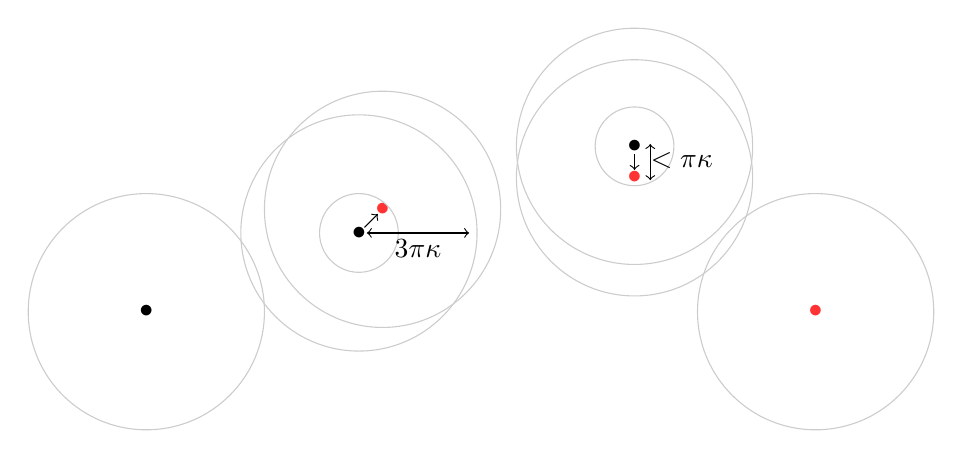
\begin{tikzpicture}
	% Pair 1
       	\draw[black] (0,0) node {$\bullet$} ;
	\draw[red!80] (.3,.3) node {$\bullet$} ; 
	\draw[->] 	(.07,.07)    	-- 	(.24,.24);
	\draw[black!20] (0,0) circle (1.5);
	\draw[black!20] (0,0) circle (0.5);
	\draw[black!20] (.3,.3) circle (1.5);
	\draw[<->]	(0.1,0)    	-- 	(1.4,0);
	\draw (0.75,-0.2)  node {$3\pi \kappa$};
	% Pair 2
	\draw[black] (3.5,1.1) node {$\bullet$} ;
	\draw[red!80] (3.5,0.7) node {$\bullet$} ; 
	\draw[->] 	(3.5,1.0)    	-- 	(3.5,0.8);
	\draw[black!20] (3.5,1.1) circle (1.5);
	\draw[black!20] (3.5,1.1) circle (0.5);
	\draw[black!20] (3.5,.7) circle (1.5);
	\draw[<->] 	(3.7,1.13)    	-- 	(3.7,0.67);
	\draw (4.1,0.92)  node {$<\pi \kappa$};
	% single black
	\draw[black] (-2.7,-1) node {$\bullet$} ;
	\draw[black!20] (-2.7,-1) circle (1.5);
	% single red
	\draw[red!80] (5.8,-1) node {$\bullet$} ;
	\draw[black!20] (5.8,-1) circle (1.5);
\end{tikzpicture}
        }
\caption{Configuration in dimension $2$ satisfying hypotheses of \thref{pairsdiracs}. The initial $\rho_0$ and final $\rho_1$ measures are composed of the black and red Dirac measures, respectively. At least 1 couple of spheres of radius $3\pi \kappa$ do not intersect for each pair of systems. We show that in that case, the geodesic is the sum of two travelling Dirac solutions (for the pairs), an on-place decreasing Dirac measure (single black) and an on place increasing Dirac measure (single red).}
\label{fig: matchingdiracs}
\end{figure}

\begin{proof}
Again we choose $\kappa=1$ without loss of generality. As for now, assume that all masses $h^i_0, h^i_1$ are strictly positive, the case of vanishing masses, i.e.\ ``single'' Dirac measures, will be fixed at the end of the proof. We aim at building an optimality certificate $\varphi \in C^1([0,1]\times \Om)$ for the candidate geodesic of the Theorem. Hence $\varphi $ should satisfy, for all $(t,x)\in [0,1]\times \Om$,
\[
\D_t \varphi +\frac12 \left( |\nabla \varphi| ^2 +  \varphi^2 \right) \leq 0
\]
and for all $t\in [0,1]$, for all $i\in \{ 1, \dots , N \}$ :
\[
\quad 
\begin{cases}
\nabla \varphi(x^i(t),t) = (x^i)'(t) \\
\varphi(x^i(t),t)=(h^i)'(t)/h^i(t) \\
\D_t \varphi +\frac12 \left( |\nabla \varphi |^2 + \varphi^2 \right) = 0 \quad  \text{for points of the form $(t,x^i(t))$}.
\end{cases}
\]

We introduce for $i\in \{1,\dots N\}$, the certificates $\varphi^i$ for the geodesics between each couple of Dirac measures $(h^i_0 \delta_{x^i_0}, h^i_1 \delta_{x^i_1})$ as defined in equation \eqref{certifddim}. The three parameters describing $\varphi^i$ are denoted $t^i_1, t^i_2$ and $\theta^i$. As $\theta^i$ is only defined up to translations, we decide from now on that $\theta^i$ is the unique such translation satisfying $\max\{ \vert x^i_0-\theta^i \vert, \vert x^i_1-\theta^i \vert \}< \pi$, which exists under our assumption that $|x_0^i - x_1^i|<\pi$. Thus, from the hypotheses in the Theorem, we have that $\min_{i \neq j}\{\vert \theta^i- \theta^j \vert \} > 4 \pi$. Now consider the \emph{binding} functions, defined for $i \in \{1,\dots,N \}$ by
\[
\varphi^i_b(t,x)=-\frac{1}{t-t^i_2} \cos(\vert x-\theta^i \vert ) + \frac{1}{t-t^i_2}. 
\]
Each $\varphi^i_b$ is in phase with $\varphi^i$ and satisfies 
\[
\varphi^i_b(t,\pi u + \theta^i)=\frac{2}{t-t_2^i}=\varphi^i(t,\pi u+ \theta^i) 
\quad \text{ and } \quad
\varphi^i_b(t,2\pi u+ \theta^i)=0
\]
for all $u\in \R^d$, $\vert u \vert = 1$ and $t\in[0,1]$. Also they are solutions to the equation $\D_t \varphi^i_b +\frac12 \left( (\nabla \varphi^i_b )^2 + (\varphi^i_b)^2 \right) = 0$. Now, as the constant zero function is a solution of this p.d.e too, we introduce
\begin{equation*}
\varphi(t,x)=
\begin{cases}
\varphi^i (t,x) & \text{if }  \vert x - \theta^i \vert \leq \pi \\
\varphi^i_b (t,x) & \text{if }  \vert x - \theta^i \vert \leq 2\pi  \text{ and } \vert x - \theta^i \vert > \pi\\
0 & \text{ otherwise.}
\end{cases}
\end{equation*}
Under the hypotheses of the Theorem, only one condition is met at a time so this function is well defined. It belongs to $C^1([0,1]\times \Om)$ because the bindings are located where the gradients vanish, on the extrema of cosines. See Figure \ref{figure certificate} to picture how the bindings are performed between the $\varphi^i$s. By construction, all hypotheses are fulfilled so that $\varphi$ be an optimality and uniqueness certificate.

Now if one or more of the $h^i_0$ or $h^i_1$ vanish, the same reasoning as in the proof of \thref{2diracs} allows to compute the distance between $\rho_0$ and $\rho_1$ (by an upper and lower bound, making the mass of vanishing Dirac measures tend to zero), and all that remains is to see that replacing the travelling Dirac solution by a Hellinger geodesic for single Dirac measures reaches that cost. 
\end{proof}

\begin{figure}%[ht]
\centering
 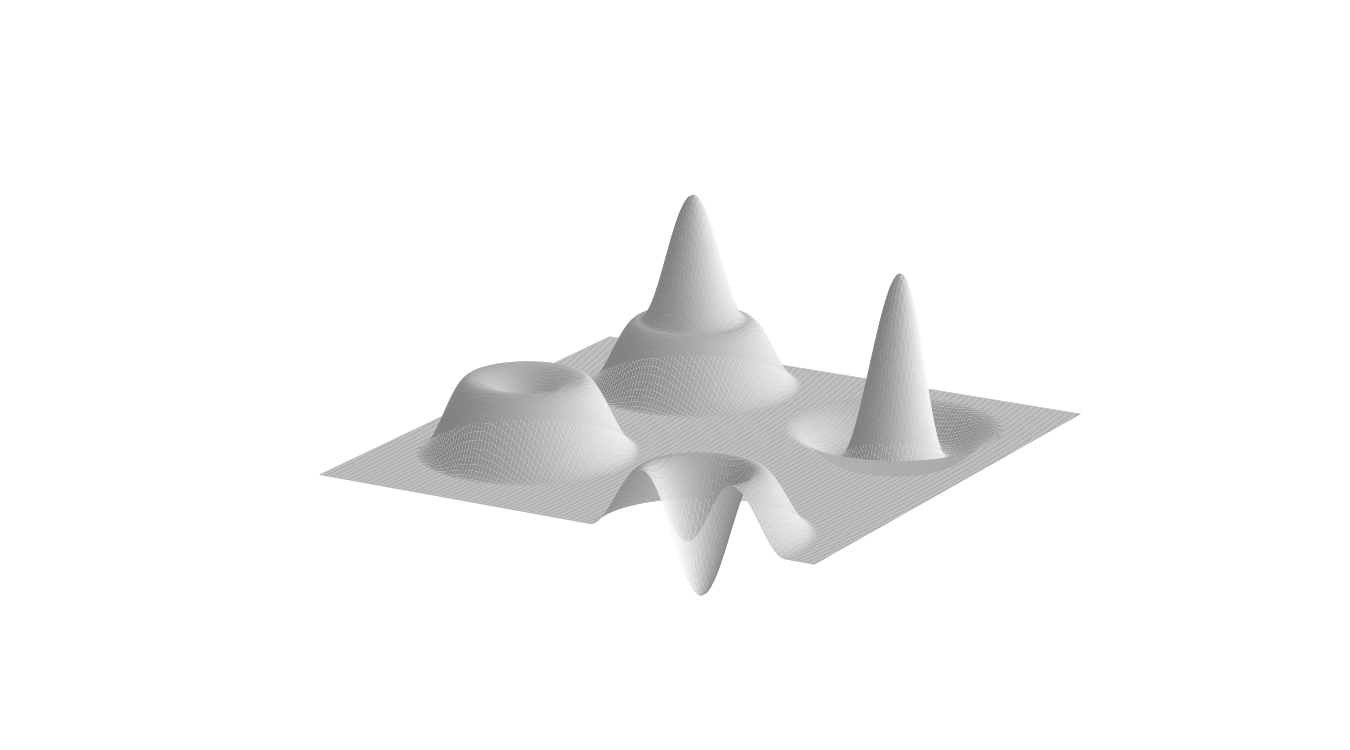
\includegraphics[trim=3cm 3cm 3cm 3cm, width=.7\linewidth]{images/certificate_dec2}%  ,clip,trim=15cm 10cm 15cm 15cm
 \caption{Example of an optimality certificate for $4$ pairs of Dirac measures, in the case $d=2$ at fixed $t$. The centers of the bumps are the $\theta^i$s. At the position $(t,x_i(t))$ of a travelling Dirac solution, the gradient gives its speed and the height gives its rate of growth.} 
 \label{figure certificate}
\end{figure}

%%%%%%%%%%%%%%%%%%%%%%%%%%%%%

% !TEX root = ../DynamicToStatic.tex

\section*{Conclusion and Perspectives}

In this paper, we presented a unified treatment of the unbalanced transport that allows for both statical and dynamical formulations. Our key findings are (i) a Riemannian submersion from a semi-direct product of groups with an $L^2$ metric to the $\WF$ metric, which leads to the computation of the sectional curvature and a Monge formulation, (ii) a new class of static optimal transport formulations involving semi-couplings, (iii) an equivalence between these static formulations and a class of dynamic formulations. Each of these contributions is of independent interest, but the synergy between the static, the dynamic and the Monge problems allows to get a clear picture of the unbalanced transportation problem. Beside these theoretical advances, we believe that a key aspect of this work is that the proposed static formulation opens the door to a new class of numerical solvers for unbalanced optimal transport. These solvers should leverage the specific structure of the cost $c$ considered for each application, a striking example being the $\WF$ cost~\eqref{eq:GeneralizedCost:OTFR}.

% we studied the geometry of a generalized optimal transport and we established a correspondence between dynamic formulations of these models and a new Kantorovich formulation. This is a key improvement for numerical efficiency.

%%%%
\section*{Acknowledgements}

The work of Bernhard Schmitzer has been supported by the Fondation Sciences Math\'ematiques de Paris. 
%
The work of Gabriel Peyr\'e has been supported by the European Research Council (ERC project SIGMA-Vision). 
%
The work of Fran\c{c}ois-Xavier Vialard has been supported by the CNRS (D\'efi Imag'in de la Mission pour l'Interdisciplinarit\'e, project CAVALIERI).
%
\\
We would like to thank Yann Brenier for stimulating discussions as well as Peter Michor, in particular for several important references.


% !TEX root = ../DynamicToStatic.tex

%%%%%%%%%%%%%%%%%%%%%%%%%
% APPENDIX
%%%%%%%%%%%%%%%%%%%%%%%%%

\appendix
%
%\begin{appendix}
\section{Wasserstein-Fisher-Rao as a Weak Metric}\label{WFRasWeak}
%%%%%%%%%%%%%%%%%%%%%%%%%%%%%%%%%%
%%%%%%%%%%%%%%%%%%%%%%%%%%%%%%%%%%
In this appendix, we show that the Wasserstein-Fisher-Rao is a weak metric in a Sobolev setting but does not admit a Levi-Civita connection. Similar results certainly hold for the Wasserstein metric. 

We will work in a smooth Sobolev setting, namely on $\Dens^s(\Omega)$ the space of $C^1$ positive functions on $\Omega$ that are in $H^s(\Omega,\R)$ for $s>d/2+1$ where $d $ is the dimension of the ambient space of $\Omega$. It is an open subset of $H^s(\Omega,\R)$. 
Note that the same results probably hold for the Wasserstein metric.

\begin{proposition}
The $\WF$ metric is a weak Riemannian metric on $\Dens^s(\Omega)$.
\end{proposition}

\begin{proof}
We use the fact that $\Dens^s(\Omega)$ is an open subset of the Hilbert space $H^s(\Omega,\R)$ to work in this coordinate system.
The tangent space of $\Dens^s(\Omega)$ is $\Dens^s(\Omega) \times H^s(\Omega,\R)$. 
Let $X \in H^s(\Omega,\R)$ be a function that will be seen as a tangent vector at any density $\rho \in \Dens^s(\Omega)$. We denote by $\WF(\rho)(X,X)$ the $\WF$ metric evaluated at the point $\rho$ on the tangent vector $X$. We have to prove that the map from $\Dens^s(\Omega) \times H^s(\Omega)$ into $\R$ defined by
$$ (\rho,X) \mapsto \WF(\rho)(X,X)$$ is smooth.
Recall that, using the formulation \eqref{HorizontalLiftFormulation}, $\WF(\rho)(X,X)$ is given by
\begin{equation}
\WF(\rho)(X,X) = \frac12 \langle L(\rho)^{-1}(X),X \rangle_{L^2(\Omega)}\,.
\end{equation}
where $L(\rho): H^{s+1}(\Omega) \mapsto H^{s-1}(\Omega)$ is the elliptic operator defined by 
\begin{equation}
L(\rho)(\phi) = -\nabla \cdot (\rho \nabla \phi) + \rho  \, \phi \,.
\end{equation} 
Therefore the smoothness of $\WF(\rho)(X,X) $ reduces to the smoothness of $L(\rho)^{-1}$ (defined with homogeneous Neumann boundary conditions) as an operator from $H^{s-1}$ into $H^{s+1}$ with respect to $\rho$. Since $L(\rho)$ is linear in $\rho$ and using the inverse function theorem on Hilbert manifolds, we get the result for the $H^{s-1}$ topology in the second variable $X$, which is even stronger than the desired result.
\end{proof}

Following \cite{SobolevMetricsCurvature}, we show the non existence of the Levi-Civita connection for the $\WF$ metric in the Sobolev setting.


\begin{proposition}\label{th:NonExistenceLC}
The Levi-Civita connection associated with the $\WF$ metric does not exist on $\Dens^s(\Omega)$.
\end{proposition}

\begin{proof}
From \cite[page 8]{SobolevMetricsCurvature}, there exists a Levi-Civita associated with a weak Riemannian metric if and only if the metric itself admits gradients with respect to itself in both variables.
Let $(\rho, X) \in \Dens^s(\Omega) \times H^s(\Omega)$ be an element of the tangent space.
The differentiation with respect to $\rho$ of $\WF(\rho)(X,X)$ gives the following $L^2$ gradient in the direction $Y \in H^s(\Omega,\R)$:
\begin{equation}
\partial_\rho \WF(\rho)(X,X)(Y) = \frac 12 \langle  |\phi|^2 + | \nabla \phi |^2 , Y \rangle_{L^2(\Omega)}\,,
\end{equation}
where $\phi = L(\rho)^{-1}(X)$. 

The gradient with respect to the $\WF$ metric is then defined as $L(\rho)(Z)$ where $Z\eqdef \frac12 (|\phi|^2 + | \nabla \phi |^2)$.
However, $Z \in H^s(\Omega)$ and therefore $L(\rho)(Z) \in H^{s-2}$. Thus, the gradient with respect to $\rho$ does not belong in general to $H^s$. Thus, the Levi-Civita does not exist.
\end{proof}
Note that the key point lies in the loss of smoothness when applying the elliptic operator.
This negative result only means that \textbf{in this $H^s$ topology}, the weak Riemannian metric $\WF$ does not admit a Levi-Civita connection. However, this result does not preclude the existence of a topology for which the Levi-Civita connection exists. 
%\begin{lemma}
%\label{lemma : continuity of WF}
%The distance $\WF$ is continuous for the weak* topology on $\mathcal{M}_+(\Omega)$.
%\end{lemma}
%
%\begin{proof}
%By the triangle inequality, we only need to show that if $\rho_n \rightharpoonup^* \rho$ then $\WF(\rho_n,\rho) \to 0$.
%If $\rho = 0$, then $\WF(\rho, \rho_n) = \sqrt{2 \rho_n(\Omega)} \to 0$. Now assume $\rho \neq 0$ and also $\rho_n \neq 0$ (since it is true eventually).
%We have 
%\[
%\WF(\rho, \rho_n) \leq \WF(\rho_n, \mnorm (\rho_{n})) + \WF(\rho,\mnorm (\rho_{n}))
%\]
%where $\mnorm (\rho_{n})$ is such that there exists $\alpha_n \in [0, + \infty[$, $\mnorm (\rho_{n})= \alpha_n \rho_{n}$ and $\mnorm (\rho_{n})(\Omega)=\rho(\Omega)$. Note that, by weak* convergence, we have that $\alpha_n \to 1$ and $W_2(\mnorm (\rho_{n}),\rho) \to 0$. But $\WF$ is upper bounded by Fisher-Rao and by $(1/2)W_2$, since those two metrics are obtained by taking the infimum of the same functional by adding the constraint $\omega=0$ and $\zeta=0$, respectively. Thus,
%\[
%\WF(\rho, \rho_{n}) \leq \delta|\sqrt{\alpha_n}-1|\sqrt{2 \rho_{n}(\Omega)} + (1/2) W_2(\mnorm (\rho_{n}),\rho) \to 0 \, . 
%\]
%\end{proof}

\section{Proof of Proposition \ref{th:ClassificationOfMetrics}}\label{sec:ProofOfClassificationOfMetrics}
\begin{proof}
For given positive functions $a, \lambda$ on $\Omega$, one has
\begin{equation}
\Phi^*(mg +  \frac{c(x)}{ m} \d m^2) = m (g + c (\d \lambda)^2) + 2c \lambda \d \lambda  \d m + \frac{c}{m} \lambda^2 \d m^2\,.
\end{equation}
Using that
$h(x,m) = m h(x) + a(x) \d m + b(x) \frac{\d m^2}{m}$,
then, the result is satisfied if and only if the following system  has a solution
\begin{equation}\label{System}
\begin{cases}
c  \,\d (\lambda^2)= a \\
c \lambda^2 =  b \,.
\end{cases}
\end{equation} 
Therefore, since $c, \lambda,b$ are positive functions, dividing the first equation by the second gives:
$$ \frac{\d (\lambda^2)}{\lambda^2} = \frac{a}{b}\,\cdot$$ 
This equation has a solution if and only if  $\frac{a}{b}$ is exact. Then, $c$ can then be deduced using the second equation of the system.

The last point consists in proving that $g \eqdef h - c (\d \lambda)^2 $ is a metric on $\Omega$. Using the relation in system \eqref{System}, we get 
$c  (\d \lambda)^2 = \frac{a^2}{4b}$. Let us consider $(v_x,v_m) \in T_{(x,m)}(M \times \R_+^*)$ for a non-zero vector $v_x$, then $mh(x)(v_x,v_x) + a(x)(v_x)v_m + \frac{b(x)}{m}v_m^2$ is a polynomial function in $v_m$ whose discriminant is necessarily strictly negative since $(v_x,v_m) \neq 0$ for all $v_m$. Therefore, we obtain 
\begin{equation}
a(x)(v_x)^2 < 4 b(x)h(x)(v_x,v_x)
\end{equation}
which gives $h(x)(v_x,v_x) - c(x) \d \lambda(x)(v_x)^2 > 0$.
\end{proof}





\bibliographystyle{spmpsci}
\bibliography{SecOrdLandBig,SecOrdLand,bibchizat,references}

%% !TEX root = ../DynamicToStatic.tex

%%%%%%%%%%%%%%%%%%%%%%%%%
% APPENDIX
%%%%%%%%%%%%%%%%%%%%%%%%%

\appendix
%
%\begin{appendix}
\section{Wasserstein-Fisher-Rao as a Weak Metric}\label{WFRasWeak}
%%%%%%%%%%%%%%%%%%%%%%%%%%%%%%%%%%
%%%%%%%%%%%%%%%%%%%%%%%%%%%%%%%%%%
In this appendix, we show that the Wasserstein-Fisher-Rao is a weak metric in a Sobolev setting but does not admit a Levi-Civita connection. Similar results certainly hold for the Wasserstein metric. 

We will work in a smooth Sobolev setting, namely on $\Dens^s(\Omega)$ the space of $C^1$ positive functions on $\Omega$ that are in $H^s(\Omega,\R)$ for $s>d/2+1$ where $d $ is the dimension of the ambient space of $\Omega$. It is an open subset of $H^s(\Omega,\R)$. 
Note that the same results probably hold for the Wasserstein metric.

\begin{proposition}
The $\WF$ metric is a weak Riemannian metric on $\Dens^s(\Omega)$.
\end{proposition}

\begin{proof}
We use the fact that $\Dens^s(\Omega)$ is an open subset of the Hilbert space $H^s(\Omega,\R)$ to work in this coordinate system.
The tangent space of $\Dens^s(\Omega)$ is $\Dens^s(\Omega) \times H^s(\Omega,\R)$. 
Let $X \in H^s(\Omega,\R)$ be a function that will be seen as a tangent vector at any density $\rho \in \Dens^s(\Omega)$. We denote by $\WF(\rho)(X,X)$ the $\WF$ metric evaluated at the point $\rho$ on the tangent vector $X$. We have to prove that the map from $\Dens^s(\Omega) \times H^s(\Omega)$ into $\R$ defined by
$$ (\rho,X) \mapsto \WF(\rho)(X,X)$$ is smooth.
Recall that, using the formulation \eqref{HorizontalLiftFormulation}, $\WF(\rho)(X,X)$ is given by
\begin{equation}
\WF(\rho)(X,X) = \frac12 \langle L(\rho)^{-1}(X),X \rangle_{L^2(\Omega)}\,.
\end{equation}
where $L(\rho): H^{s+1}(\Omega) \mapsto H^{s-1}(\Omega)$ is the elliptic operator defined by 
\begin{equation}
L(\rho)(\phi) = -\nabla \cdot (\rho \nabla \phi) + \rho  \, \phi \,.
\end{equation} 
Therefore the smoothness of $\WF(\rho)(X,X) $ reduces to the smoothness of $L(\rho)^{-1}$ (defined with homogeneous Neumann boundary conditions) as an operator from $H^{s-1}$ into $H^{s+1}$ with respect to $\rho$. Since $L(\rho)$ is linear in $\rho$ and using the inverse function theorem on Hilbert manifolds, we get the result for the $H^{s-1}$ topology in the second variable $X$, which is even stronger than the desired result.
\end{proof}

Following \cite{SobolevMetricsCurvature}, we show the non existence of the Levi-Civita connection for the $\WF$ metric in the Sobolev setting.


\begin{proposition}\label{th:NonExistenceLC}
The Levi-Civita connection associated with the $\WF$ metric does not exist on $\Dens^s(\Omega)$.
\end{proposition}

\begin{proof}
From \cite[page 8]{SobolevMetricsCurvature}, there exists a Levi-Civita associated with a weak Riemannian metric if and only if the metric itself admits gradients with respect to itself in both variables.
Let $(\rho, X) \in \Dens^s(\Omega) \times H^s(\Omega)$ be an element of the tangent space.
The differentiation with respect to $\rho$ of $\WF(\rho)(X,X)$ gives the following $L^2$ gradient in the direction $Y \in H^s(\Omega,\R)$:
\begin{equation}
\partial_\rho \WF(\rho)(X,X)(Y) = \frac 12 \langle  |\phi|^2 + | \nabla \phi |^2 , Y \rangle_{L^2(\Omega)}\,,
\end{equation}
where $\phi = L(\rho)^{-1}(X)$. 

The gradient with respect to the $\WF$ metric is then defined as $L(\rho)(Z)$ where $Z\eqdef \frac12 (|\phi|^2 + | \nabla \phi |^2)$.
However, $Z \in H^s(\Omega)$ and therefore $L(\rho)(Z) \in H^{s-2}$. Thus, the gradient with respect to $\rho$ does not belong in general to $H^s$. Thus, the Levi-Civita does not exist.
\end{proof}
Note that the key point lies in the loss of smoothness when applying the elliptic operator.
This negative result only means that \textbf{in this $H^s$ topology}, the weak Riemannian metric $\WF$ does not admit a Levi-Civita connection. However, this result does not preclude the existence of a topology for which the Levi-Civita connection exists. 
%\begin{lemma}
%\label{lemma : continuity of WF}
%The distance $\WF$ is continuous for the weak* topology on $\mathcal{M}_+(\Omega)$.
%\end{lemma}
%
%\begin{proof}
%By the triangle inequality, we only need to show that if $\rho_n \rightharpoonup^* \rho$ then $\WF(\rho_n,\rho) \to 0$.
%If $\rho = 0$, then $\WF(\rho, \rho_n) = \sqrt{2 \rho_n(\Omega)} \to 0$. Now assume $\rho \neq 0$ and also $\rho_n \neq 0$ (since it is true eventually).
%We have 
%\[
%\WF(\rho, \rho_n) \leq \WF(\rho_n, \mnorm (\rho_{n})) + \WF(\rho,\mnorm (\rho_{n}))
%\]
%where $\mnorm (\rho_{n})$ is such that there exists $\alpha_n \in [0, + \infty[$, $\mnorm (\rho_{n})= \alpha_n \rho_{n}$ and $\mnorm (\rho_{n})(\Omega)=\rho(\Omega)$. Note that, by weak* convergence, we have that $\alpha_n \to 1$ and $W_2(\mnorm (\rho_{n}),\rho) \to 0$. But $\WF$ is upper bounded by Fisher-Rao and by $(1/2)W_2$, since those two metrics are obtained by taking the infimum of the same functional by adding the constraint $\omega=0$ and $\zeta=0$, respectively. Thus,
%\[
%\WF(\rho, \rho_{n}) \leq \delta|\sqrt{\alpha_n}-1|\sqrt{2 \rho_{n}(\Omega)} + (1/2) W_2(\mnorm (\rho_{n}),\rho) \to 0 \, . 
%\]
%\end{proof}

\section{Proof of Proposition \ref{th:ClassificationOfMetrics}}\label{sec:ProofOfClassificationOfMetrics}
\begin{proof}
For given positive functions $a, \lambda$ on $\Omega$, one has
\begin{equation}
\Phi^*(mg +  \frac{c(x)}{ m} \d m^2) = m (g + c (\d \lambda)^2) + 2c \lambda \d \lambda  \d m + \frac{c}{m} \lambda^2 \d m^2\,.
\end{equation}
Using that
$h(x,m) = m h(x) + a(x) \d m + b(x) \frac{\d m^2}{m}$,
then, the result is satisfied if and only if the following system  has a solution
\begin{equation}\label{System}
\begin{cases}
c  \,\d (\lambda^2)= a \\
c \lambda^2 =  b \,.
\end{cases}
\end{equation} 
Therefore, since $c, \lambda,b$ are positive functions, dividing the first equation by the second gives:
$$ \frac{\d (\lambda^2)}{\lambda^2} = \frac{a}{b}\,\cdot$$ 
This equation has a solution if and only if  $\frac{a}{b}$ is exact. Then, $c$ can then be deduced using the second equation of the system.

The last point consists in proving that $g \eqdef h - c (\d \lambda)^2 $ is a metric on $\Omega$. Using the relation in system \eqref{System}, we get 
$c  (\d \lambda)^2 = \frac{a^2}{4b}$. Let us consider $(v_x,v_m) \in T_{(x,m)}(M \times \R_+^*)$ for a non-zero vector $v_x$, then $mh(x)(v_x,v_x) + a(x)(v_x)v_m + \frac{b(x)}{m}v_m^2$ is a polynomial function in $v_m$ whose discriminant is necessarily strictly negative since $(v_x,v_m) \neq 0$ for all $v_m$. Therefore, we obtain 
\begin{equation}
a(x)(v_x)^2 < 4 b(x)h(x)(v_x,v_x)
\end{equation}
which gives $h(x)(v_x,v_x) - c(x) \d \lambda(x)(v_x)^2 > 0$.
\end{proof}





\end{document}
